\documentclass[12pt,a4paper,twoside,openright]{book}
\pagestyle{headings} % page style (for heading etc)

\usepackage[numbers,sort&compress]{natbib}
\bibliographystyle{plos2015}

\usepackage[a4paper]{meta-donnees} % University template
\usepackage[utf8]{inputenc} % UTF-8 for accents
\usepackage[T1]{fontenc} % UTF-8 for accents
\usepackage[english,french]{babel} % for langages
%\usepackage{epigraph} % for quotations at the beginning of each chapter
%\setlength{\epigraphwidth}{15cm}

% amsmath and amssymb packages, useful for mathematical formulas and symbols
\usepackage{amsmath,amssymb,amsfonts,mathrsfs}

\usepackage{graphicx} % no idea but was needed in the suppinfo of chapter 2

% Use nameref to cite supporting information files (see Supporting Information section for more info)
\usepackage{nameref}

% hyperlink
\usepackage{hyperref}
\usepackage{xcolor}
\hypersetup{
    colorlinks = true,
    allcolors = {blue},
    linktocpage = true, % for line break in table of contents
}
\usepackage{doi}
\usepackage[hyphenbreaks]{breakurl}

% Remove brackets from numbering in List of References
\makeatletter
\renewcommand{\@biblabel}[1]{\quad#1.}
\makeatother

% For table of content line break
%\usepackage{tocstyle}
%\usetocstyle{standard}

% To keep figures in section
\usepackage[section]{placeins}

% To insert pdf (the sequences in appendix)
\usepackage{pdfpages}

% For genetic sequences
\usepackage{seqsplit}


%%%%%%%%%%% Custom environment %%%%%%%%%%%
\newenvironment{acknowledgements}{
\newpage
\null \vspace{\stretch{1}}
\begin{center}\bfseries Remerciements \end{center}
}
{\vfill \null}

\newenvironment{abstract}{
\clearpage
\begin{center}\bfseries \abstractname \end{center}
}
{\null}

\newenvironment{author-summary}{
\begin{center}\bfseries Non-technical summary of the work \end{center}
}
{\vfill \null}

\newenvironment{resume-vulgaire}{
\begin{center}\bfseries Résumé pour le grand public \end{center}
}
{\vfill \null}

\newenvironment{chapter_summary}[1]{
\section*{Résumé du Chapitre \thechapter : #1}
}
{\null}


%% For chapter mark
%\makeatletter
%\g@addto@macro{\frontmatter}{
%    \renewcommand{\chaptermark}[1]{%
%        \markboth{#1}{}%
%    }    
%}
%\g@addto@macro{\mainmatter}{
%    \renewcommand{\chaptermark}[1]{%
%        \markboth{Chapter \thechapter{}: #1}{}%
%    }    
%}
%\g@addto@macro{\backmatter}{
%    \renewcommand{\chaptermark}[1]{%
%        \markboth{#1}{}%
%    }    
%}
%\makeatother

%%%%%%%%%%%%%%%%%%%%%%%%%%%%%%%%%%%%%%%%%%%

%%%%%%%%%%%%% Custom commands %%%%%%%%%%%%%

%%%%%%%%%%%%%%%%%%%%%%%%%%%%%%%%%%%%%%%%%%%

%%%%%% FOR MANUAL REF%%%%%
\makeatletter
\newcommand{\manuallabel}[2]{\def\@currentlabel{#2}\label{#1}}
\makeatother
%%%%%%%%%%%%%%%%%%%%%%%%%%%%%%%%


%%%%%%%%%%%%%%%%%%%%%%%%%%%%%%%%%%%%%%%%%%%%%%%%%%%%%%%%%%%%%%%%%%%%%%%%%%%%%%%%%%%%%%%%%%%%%%%%

\begin{document}

% les lignes en bas sont à insérer obligatoirement après \begin{document}

%%%%%%%%%%%%%%%%%%%%%%%%%%%%%%%%%%%%%%%%%%%%%%%%%%%%%%
%%             Commandes Meta-données               %%
%%   à renseigner par les auteurs pour générer      %%
%%     la couverture modèle Univ. Grenoble          %%
%%%%%%%%%%%%%%%%%%%%%%%%%%%%%%%%%%%%%%%%%%%%%%%%%%%%%%

%\Sethpageshift{-8mm}   %%optionnel : à décommenter si besoin pour ajout d'espace afin de center la couvérture horizontalement (valeur par défaut est -5.5mm)
%\Setvpageshift{0mm}   %%optionnel : à décommenter si besoin pour ajout d'espace afin de center la couvérture verticalement (valeur par défaut est -15.5mm)

%\Universite{}    %%optionnel : à décommenter et à renseigenr si vous voulez changer le non d'université
%\Grade{}         %%optionnel : à décommenter et à renseigenr si vous voulez changer le grade
\Specialite{Biologie cellulaire}
\Arrete{7 Ao\^ut 2006}
\Auteur{Nils GIORDANO}
\Directeur{Johannes GEISELMANN}
\CoDirecteur{Hidde DE JONG}
\Laboratoire{Laboratoire Interdisciplinaire de Physique}
\EcoleDoctorale{Ecole doctorale Chimie et Science du Vivant}         
\Titre{Microbial growth control in shifting environments}
\Soustitre{Theoretical and experimental study of resource allocation in \textit{Escherichia coli}}      %%optionnel : à décommenter et à renseigenr si présence d'un sous-titre de thèse
\Depot{}       


% Commande pour création de nouvelles catégories dans le jury:
%\UGTNewJuryCategory{...NomDeLaCategorie...}{...Definition...}
% Exemple \UGTNewJuryCategory{UGTFamille}{Membre de la famille} que nous ajoutons dans la commande \Jury ci-dessous sous la forme \UGTFamille{Jean Rousseau}{(...titre_et_affiliation...s'il_y_en_a...)}

\Jury{
%\UGTPresident{M, Olivier BERNARD}{Chargé de recherche, Inria, Nice -- Sophia-Antipolis (à confirmer pour président)}     %% 2ème examinateur
%\UGTPresidente{...Civilité, Prénom-et-Nom...}{...titre-et-affiliation...}

\UGTRapporteur{M, Matthew SCOTT}{Associate Professor, Department of Applied Mathematics, University of Waterloo (CA)}      %% 1er rapporteur
\UGTRapporteur{M, Guy-Bart STAN}{Reader, Department of Bioengineering, Imperial College London (U.K.)}      %% second rapporteur

\UGTExaminateur{M, Olivier BERNARD}{Chargé de recherche, Inria, Nice -- Sophia-Antipolis}     %% 2ème examinateur
\UGTExaminateur{M, Matthieu JULES}{Chargé de recherche, Inra, Grignon}     %% 1er examinateur
\UGTExaminatrice{Mme, Irina MIHALCESCU}{Maître de conférence, Université Grenoble Alpes, LIPhy}    %% 3ème examinateur

\begin{center}
\noindent\rule{4cm}{0.1pt}
\end{center}

\UGTInvite{M, Jean-Luc GOUZÉ}{Directeur de recherche, Inria, Nice -- Sophia-Antipolis}
%\UGTInvitee{...Civilité, Prénom-et-Nom...}{...titre-et-affiliation...}

\UGTDirecteur{M, Johannes GEISELMANN}{Professeur, Université Grenoble Alpes, LIPhy}       %% Directeur de thèse
\UGTCoDirecteur{M, Hidde DE JONG}{Directeur de recherche, Inria, Grenoble -- Rhône-Alpes}     %% Co-Directeur de thèse s'il y en a
}


\MakeUGthesePDG    %% très important pour générer la couverture de thèse

%\cleardoublepage
\null \vspace{\stretch{1}}
\begin{flushright}
\textit{(dédicace ici)}
\end{flushright}
\vspace{\stretch{2}}\null

%\cleardoublepage
\begin{acknowledgements}
(remerciements ici)
\end{acknowledgements}

\selectlanguage{english}
\begin{abstract}
\lipsum[2]
\end{abstract}

\selectlanguage{french}
\begin{abstract}
\lipsum[2]
\end{abstract}
\selectlanguage{english}


\tableofcontents

%\frontmatter
%\input{Chapters/introduction_summary}
%\mainmatter
\chapter{Introduction}

\textit{There's an infinity of things that have never been done before, and most of those things are not worth doing.} -- Jeremy Fox, \textit{Dynamic Ecology (2016)}~\cite{fox_how_2016}

\selectlanguage{french}
\section*{Résumé en français}

Dans cette section... (env. 1-2 pages)
\selectlanguage{english}

\begin{center}
\noindent\rule{4cm}{0.1pt}
\end{center}

\section{Context}
\label{sec:context}

\subsection{Self-replication is a resource allocation problem}

At every moment of our lives, we are surrounded by billions of microscopic organisms.
They sustain themselves by collecting energy from their environment, in the form of organic matter, highly reactive chemicals, or light~\cite{madigan_biology_2006,schaechter_microbe_2006}.
While most of our cells are kept in a stable and friendly internal environment (temperature, oxygenation, nutrient abundance, ...), microorganisms have evolved to constantly adapt their physiology to strongly variable environments.
Not without a certain success, because microbes have been found to survive almost everywhere, sometimes in the strangest places that were initially thought unsuitable for life~\cite{rothschild_life_2001,nicholson_transcriptomic_2012,madigan_biology_2006,schaechter_microbe_2006}.
Such ubiquity translates a strong potential for adaptation.
Even the model organism \textit{Escherichia coli}, a bacteria first isolated from our intestinal track, is capable of growing on dozens of different carbon sources through changes in the expression of thousands of genes\cite{zimmer_microcosm:_2009}.

Microorganisms, along with all living cells, are mainly constituted of polymers (DNA, RNA, Proteins) made of many repeated sub-units (nucleotides, amino acids).
The information about their sequences is stored in the form of genes on the DNA.
Gene expression is the process by which this information is used in the synthesis of a functional final product (protein or RNA).
The gene expression machinery (itself constituted of RNA and proteins) synthesizes the gene products after binding to gene promoters, which are target sequences on the DNA.
In a given cell, they are roughly as many different target sequences as genes, which ensures that not all products are synthesized at the same rate.
Furthermore, some of these products specifically bind some promoters and stimulates or represses the promoter activity, hence, the gene expression.
They are called transcription factors and allow, among other mechanisms, the regulation of cell composition.

The reorganization of gene expression controls the abundance of enzymes and ribozymes that catalyzes the biochemical reactions allowing the cell to perform different functions.
For instance, assimilating a given nutrient involves the synthesis of the corresponding uptake protein and of the metabolic enzymes converting the nutrients into reductive power, nucleotides and amino acids~\cite{schaechter_microbe_2006}.
These precursors are then used to produce new macromolecules, closing the loop of self-replication.
In order to optimize the overall process in different environmental conditions, the cell must adjust the abundance of every enzyme involved in this network of biochemical reactions.
By doing so, the cell actually resolves a resource allocation problem, where a common wealth (precursors) has to be distributed over thousands of potential beneficiaries (proteins and other macromolecules).

\subsection{Optimizing biomass production yields a competitive advantage}

Which resource allocations are optimal for a living cell?
Systems capable of Darwinian evolution sustain themselves on the long term by \textit{fitting} to their environment.
Living cells with the best \textit{fitness} are more likely to survive, replicate, and through long-term competition, eliminate their siblings.
The optimization criteria that quantitatively measure \textit{fitness} are called \textit{fitness factors}.
Whether they apply at the species, the population, the organism, or even the gene level has long been debated~\cite{dawkins_selfish_1976}.
An optimal resource allocation would be a gene expression scheme that maximizes the fitness factors.
But since fitness factors have to take into account the ability to survive, reproduce, and compete with other organisms in a given (sometimes changing) environment, they are often context-dependent and highly difficult to identify.

For this reason, there is no consensus about what constitute the main fitness factors of microorganisms.
Competition for common resources seems to favor the maximization of offspring, in the sense that a replicator with more descendants will outnumber its competitors in the long term~\cite{dawkins_selfish_1976}.
It is unclear, however, how this general principle translates into their physiological behaviors.
For instance, the use of genome-scale metabolic network models have shown that the metabolism maximizes the production either of biomass or available energy (ATP) depending on the environmental condition~\cite{schuetz_systematic_2007}.
But we can also found different strategies when the biomass production is at play.
Bacteria can either optimize their production yield (taking its time to make the most of the nutrient) or their production rate (growing quickly while wasting part of the nutrient potential), the later being favored in fluctuating or poor environments~\cite{frank_tradeoff_2010,maclean_tragedy_2008}, a result that has also been confirmed in yeast~\cite{schuster_maximization_2008}.
Overall, it seems that cell optimality drifts in a multidimensional space and involves making several trade-offs that strongly depend on the environmental context~\cite{schuetz_multidimensional_2012}.

Nevertheless, numerous studies have shown that considering growth rate maximization confers a good predictive power of microorganism physiology.
When cultivated in minimal medium with acetate or succinate, \textit{Escherichia coli} uptake rates are correctly predicted by assuming that the metabolic network operates in a mode that maximizes growth rate~\cite{edwards_silico_2001}.
This result is not general though, and depends on the carbon source and strain used~\cite{ibarra_escherichia_2002}.
But even in those cases, the metabolic networks evolve rapidly towards growth-rate maximization if a constant nutrient-providing environment is maintained~\cite{ibarra_escherichia_2002}.
The mutants obtained present modications in the regulation of the synthesis of metabolic enzymes~\cite{lewis_omic_2010}, indicating that not only the efficiency of the enzymes is affected, but also their abundance and thus the cellular composition.
Overall, with the currently available knowledge and its limitations (discussed in section~\ref{chap:discussion}), growth-rate maximization sounds like a rational choice to understand the growth strategies of microorganisms~\cite{molenaar_shifts_2009}.

\subsection{Growth laws are universal strategies employed by microorganisms}

One of the first attempt to formalize microorganism physiology into elegant, fundamental laws was the discovery of Monod's law more than sixty years ago~\cite{monod_growth_1949}.
This empirical relationship states that the growth rate $\mu$ [\texttt{div.h\textsuperscript{-1}}] of \textit{Escherichia coli} is a hyperbolic function of the concentration of the limiting nutrient $C$ [\texttt{mol.L\textsuperscript{-1}}], such that
\begin{equation}
\label{eq:monod_law}
\mu = \mu_K \frac{C}{K_C + C}
\end{equation}
with $\mu_K$ and $K_C$ two constants depending on the quality of the nutrient (Fig~\ref{fig:monod_law}).
It is remarkable that the growth rate, a parameter that depends on the use and production of thousands of proteins, can be so easily predicted by a simple relation.
What is even more remarkable is that this relation is rather universal.
Despite some adjustments (the Droop model being a well-known example~\cite{droop_thoughts_1973}), the relation holds for most microorganisms: the growth rate increases with the abundance of the limiting nutrient, up to a point beyond which they cannot grow any faster~\cite{koch_why_1988}.

\begin{figure}[tb]
\centering
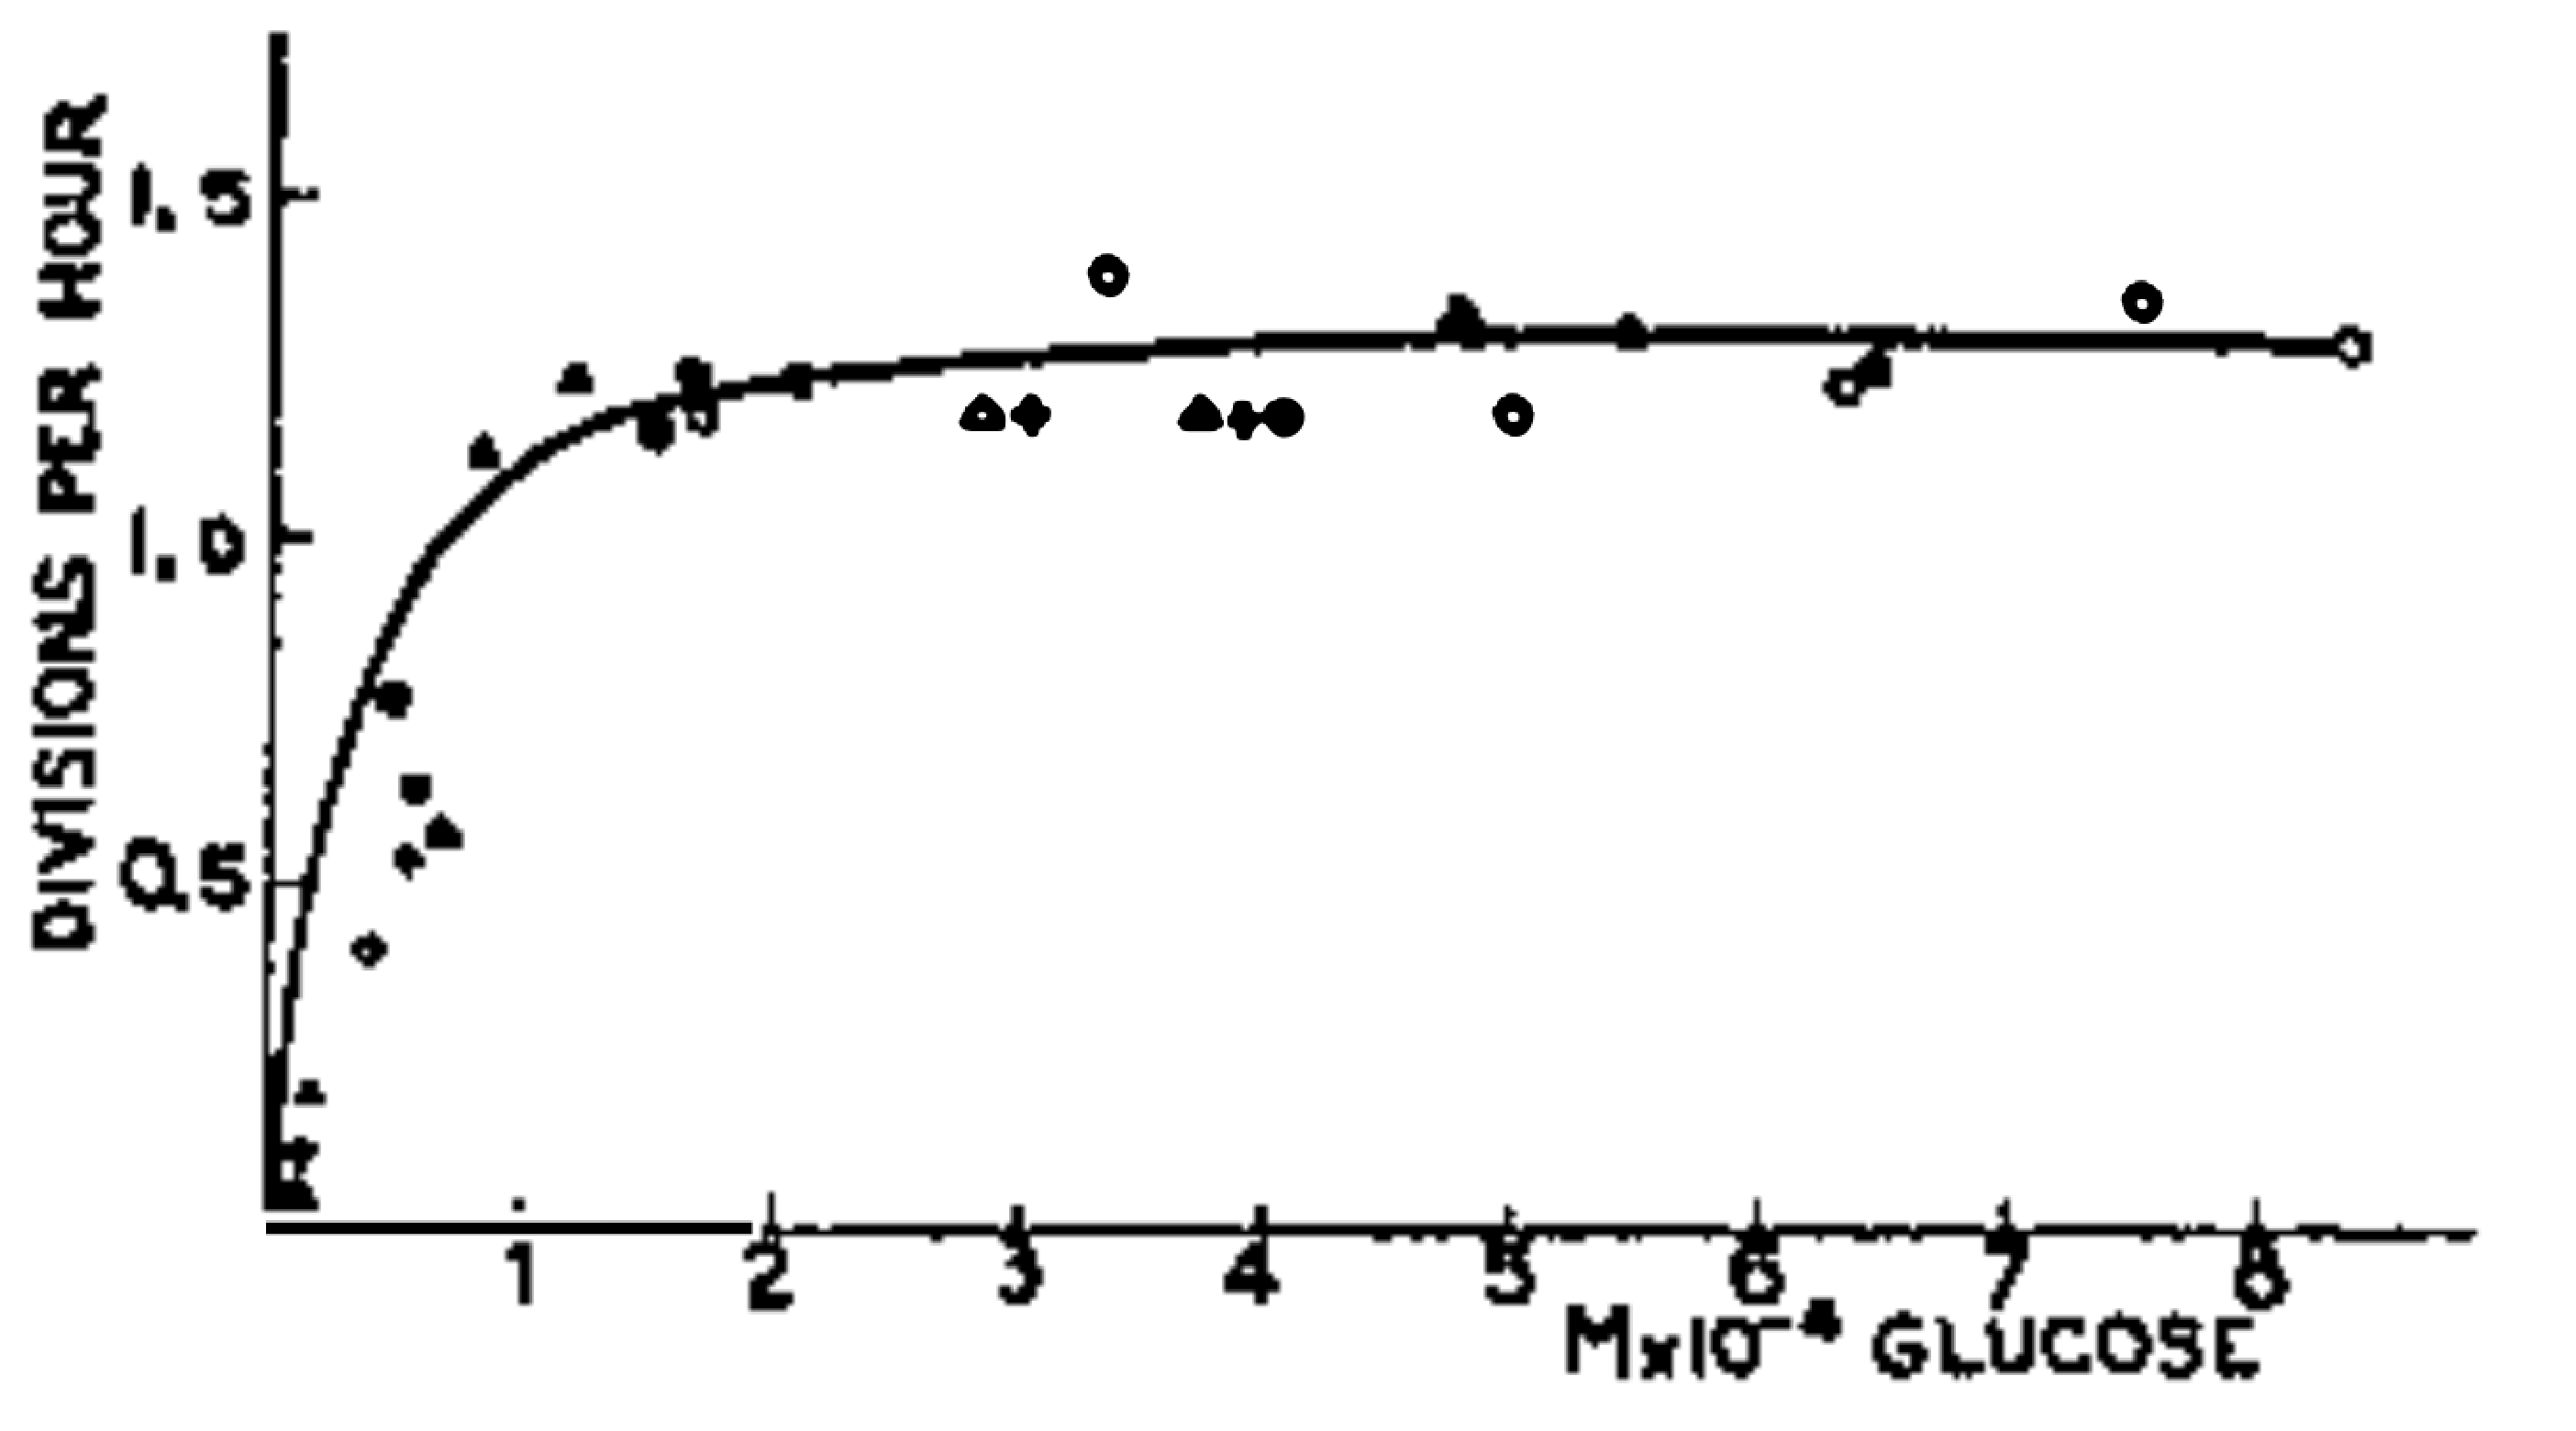
\includegraphics[height=5cm]{./Fig/Chapter1/monod_law.eps}
\caption{
\textbf{Monod law, reproduced from~\cite{monod_growth_1949}.}
Monod has been a pioneer in the formalization of microbial growth into fundamental, coarse-grained relationships.
This figure displays the growth rate (in number of divisions per hour) of \textit{Escherichia coli} in a synthetic minimal medium at 37$^{\circ}$C containing different concentrations of glucose (a common carbon source).
As the concentration of glucose increases, the growth rate of \textit{E. coli} does so by following the hyperbolic relationship described in Eq~\ref{eq:monod_law}.
Solid line is drawn with $\mu_K = 1.35$ div.h\textsuperscript{-1}, and $K_C = 0.22 \cdot 10^{-4}$ mol.L\textsuperscript{-1}.
}
\label{fig:monod_law}
\end{figure}

The production of every component of the cell is controlled by a complex network of regulatory interactions.
But an obvious constraint is that at steady state, the synthesis rate of all individual components must be proportional to the growth rate in order to compensate for growth dilution~\cite{monod_growth_1949}.
Many physiological parameters (like mass of DNA, RNA and proteins) are thus functions of the growth rate alone, regardless of the environmental conditions~\cite{schaechter_dependency_1958,bremer_modulation_1996}.
These so-called growth laws were carefully measured~\cite{bremer_modulation_1996} and are still used today in the quantitative understanding of growth control in microorganisms~\cite{ehrenberg_mediumdependent_2012}.
Recently, the topic was revitalized through the work of Scott \textit{et al}~\cite{scott_bacterial_2011}.
They focused on the ribosome concentration, a physiological parameter that was long known to vary linearly with the growth rate in microorganisms (Fig~\ref{fig:scott_rnaprot}).
By measuring it under different environmental perturbations of the protein synthesis machinery, they built a coarse-grained model describing proteome resource allocation~\cite{scott_emergence_2014}.
It has allowed to show that, whatever the details of the molecular implementation (differing between organisms), this growth law emerges from the underlying principles of robustness and optimization imposed by natural selection, especially growth-rate maximization in every conditions~\cite{scott_emergence_2014}.

\begin{figure}[tb]
\centering
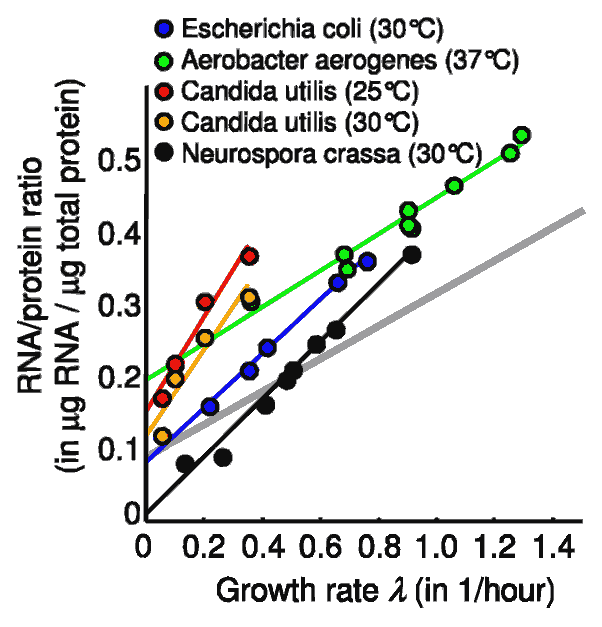
\includegraphics[height=7cm]{./Fig/Chapter1/scott_rnaprot.eps}
\caption{
\textbf{The growth law of ribosomal abundance (figure reproduced from Fig~S1 in~\cite{scott_interdependence_2010}).}
For a variety of carbon nutrients and their corresponding steady-state growth rate, the RNA/protein ratio is linearly correlated with the growth rate, a relation that holds for many species of microorganisms.
This ratio is correlated with the fraction of ribosome-affiliated proteins, and therefore with the relative abundance of ribosomes in the cell.
}
\label{fig:scott_rnaprot}
\end{figure}

\subsection{Static versus dynamical perspective on growth}

The growth laws cited above apply at steady state, where all intensive properties of the cell are time-invariant~\cite{schaechter_microbe_2006,fishov_microbial_1995}.
It means that the properties independent of the cell volume or mass (temperature, concentrations, ...) are constant over time, even though the cell is still growing.
It requires that the components of the cell "increases by the same factor over a time interval", which have motivated the creation of the term balanced growth~\cite{campbell_synchronization_1957}.
Experimentally, this growth scenario has been used as a standard because it improves reproducibility, in that samplings are no longer time-sensitive~\cite{schaechter_microbe_2006}.
It can be easily achieved in the laboratory either in continuous culture, where the substrate is continually supplied, or in batch conditions if the substrate is in high excess (Fig~\ref{fig:growth_curve}).
This approach has been beneficial to mathematical modeling because considering the system at steady state reduces the complexity of the underlying dynamical systems, allowing to build and analyze huge genome-scale models that encapsulate the enzymatic diversity of living cells~\cite{orth_what_2010}.

\begin{figure}[p]
\centering
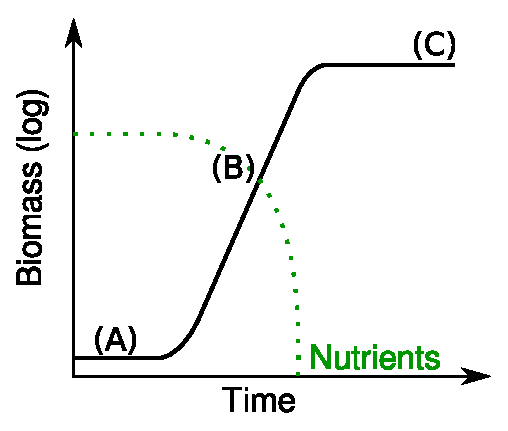
\includegraphics[height=6cm]{./Fig/Chapter1/growth_curve.eps}
\caption{
\textbf{The different phases of a typical growth curve}.
During a typical batch growth scenario, biomass accumulates (black thick line) whereas nutrients are consumed until depletion (green dashed line)~\cite{schaechter_microbe_2006}.
(A) The lag phase is a variable period of time during which the organism adapt to the new medium~\cite{swinnen_predictive_2004}.
It is hard to study experimentaly and is known to be affected by the pre-culturing history of the strain~\cite{ng_damage_1962,dufrenne_effect_1997,shaw_effect_1967}, the magnitude and the rate of the change between the past and present environments~\cite{mcmeekin_predictive_2002}, and other hard-to-control environmental conditions~\cite{cheroutre-vialette_application_2002}.
(B) The steady-state (or balanced-growth) phase is characterized by an exponential production of biomass.
Its characteristics are time-invariant and reproducible, which has made it a standard for microbial growth studies~\cite{schaechter_microbe_2006}.
This phase can be extended for hundreds of generations in continuous cultures, by the constant addition of fresh medium~\cite{wang_robust_2010}.
As represented here, nutrients are quickly depleted in batch conditions, which does not allow to maintain steady-state growth for a long period of time.
(C) The stationary phase occurs after the depletion of the limiting nutrients in the medium~\cite{chubukov_environmental_2014,schaechter_microbe_2006}.
In natural conditions, microorganisms usually encounter poor media and spend most of their time in stationary phase~\cite{mcarthur_microbial_2006,menge_nitrogen_2012,hobbie_microbes_2013}.
Some species which have evolved long-term resistance mechanisms, like sporulation~\cite{stragier_molecular_1996} or cannibalism~\cite{gonzalez-pastor_cannibalism:_2011}, can survive particularly long stationary phases.
}
\label{fig:growth_curve}
\end{figure}

Although balanced growth is convenient from an experimental and theoretical point of view, it is widely admitted that microorganisms rarely encounter this state in nature~\cite{schaechter_microbe_2006}.
Steady-state growth requires stable conditions over a long period of time, but microorganisms live in
environments where the key elements, such as carbon, nitrogen or phosphorus, are quickly depleted by the competitors as soon as they become available~\cite{mcarthur_microbial_2006,menge_nitrogen_2012,hobbie_microbes_2013}, a consideration that also holds for the lab strains on which growth laws are studied~\cite{savageau_escherichia_1983,savageau_demand_1998,blount_unexhausted_2015,vanelsas_survival_2011}.
Why would microorganisms be optimal for a state they have barely encountered during their evolution?
Are we missing something by studying in stable, unchanging conditions, systems that were in fact selected to cope with environmental variations?

\section{Problem statement}

Microbial growth is essentially a resource allocation problem that can be summarized in simple, fundamental growth laws.
Though established empirically, those laws are elegantly explained if we consider that microorganisms behave in way that optimizes their biomass production.
However, these laws describe growth in stable environments, but it is hard to imagine how natural selection could have made microorganisms optimal for conditions they rarely encounter.
This motivates the study of growth laws through a dynamical perspective, that is, in a changing environment, and leads us to the following problem statement: \textbf{Which strategies microorganisms follow to dynamically reallocate their resources after a change in the environment?}
The development of this question prompts the following investigations.

What are the best strategies of resource allocation if, like for the steady-state growth laws, the biomass production is kept as the only optimization criteria?
Through answering this question, we could assess to which extend the features of dynamical optimization differ from the steady-state optimization.
In other words, it would test our verbal hypothesis that motivated a dynamical perspective on growth: the fact that we expect evolutionary pressure to apply differently between dynamic and stable conditions.
This requires to translate the problem in the mathematical world, through the development of a proof-of-concept model of resource allocation in bacterial cells, and the theoretical determination of the optimal dynamical allocation of resources following a change in the environment.

How could one measure empirically the resource allocation during a growth transition?
The model will help us to establish actual resource allocation strategies that optimize biomass production during an environmental change.
However, it will not be able to tell us if microorganism actually care to optimize such a criterion.
We need though the possibility to measure biomass accumulation and changes in resource allocation when a shift is made in the environment.
This would require a way to dynamically track the abundance of key macromolecules in living cells, while establishing an experimental set-up that temper the inherent variability of dynamical experimental studies of microbial growth.

\section{Related work}

\subsection{Modeling growth of microorganisms}

My recent experience as a teacher taught me that, as of today, a lot of students in biology do not like mathematics very much.
Since mathematics is the main language of modeling, this has often made it difficult for me to convince them that modeling is of key importance for biologists.
However, while mathematics is the language, it is not the essence of modeling.
Generally speaking, a model depicts and simplifies reality.
Maps, sketches, or pictures satisfy this definition, as do graphs, sets of equations, or even the DNA sequences stored in a text file on a computer.
In other words, depicting and simplifying reality makes you a modeler, not so much drawing equations on a board.
But this does not change the fact that mathematics are powerful tools for formulating and analyzing models~\cite{servedio_not_2014,mcgill_calm_2013}.

What makes mathematical modeling so useful in microbial growth studies?
Evolutionary biology is a good instance of field that has been resorting for a long time on mathematical modeling~\cite{servedio_not_2014}.
The large time and population scales at which evolutionary processes occur truly impede most of the experimental work, despite some attempts on organisms with a short generation time~\cite{elena_evolution_2003}.
Besides, microbiology is a field particularly prone to experimental study.
A growth curve as presented in Fig.~\ref{fig:growth_curve} can be made in a day, so the limitations of evolutionary biology should not apply to microbial growth studies.
Why care to mimic reality on a computer when we can just directly bend it to our will~\cite{hillis_why_1993}?
The last decades have strongly challenged this viewpoint: as knowledge and data on microbes accumulated, the need for a systemic understanding of biology was more and more pressing~\cite{alon_introduction_2006,kremling_systems_2013}.

Microbial physiology results from the interplay of thousands of chemical reactions that are not necessarily relevant in any given situation~\cite{schaechter_microbe_2006}.
These reactions occurs on short time scales, and are controlled by several layers of regulatory mechanisms that can only be understood through evolutionary considerations.
As a consequence, even the simplest verbal hypothesis can resist direct empirical testing.
But abstracting away complexity is the purpose of mathematical models.
The overwhelming number of variables and time scales can be dealt with by choosing the correct framework.
When working on a model, the microbe behaviors are abstracted into a world of clearly stated rules, where logical reasoning can be applied~\cite{servedio_not_2014,mcgill_calm_2013}.
Predictions can be made, "unpacked" into our real world, and confronted with experimental testing.

Modeling was particularly helpful to unveil how metabolic networks operate.
For an increasing number of microorganisms, we are now able to draw quasi-exhaustive maps of their metabolic reactions.
For instance, the most recent genome-scale reconstruction of \textit{E. coli} metabolism contains 1366 genes, 2251 metabolic reactions, and 1136 unique metabolites~\cite{orth_comprehensive_2011}.
Such a number of variables might seem overwhelming, and making sense of these knowledge is rarely straightforward.
Which reactions are important, and in which environmental conditions?
Can we predict how perturbations will affect a given metabolic network?
Do fundamental regularities exist between different metabolic networks, from different species?

This apparent complexity does not impede a mathematical studies of metabolic networks.
Constraint-based modeling is a framework that abstracts away the unknown kinetics and represents the metabolic reactions by steady-state fluxes to which physico-chemical constraints can be applied, e.g. compartmentalization, mass conservation, molecular crowding, and thermodynamic directionality~\cite{ebrahim_cobrapy_2013}.
In other words, through constraints imposed to the metabolic networks, it provides a space of admissible flux distributions, eliminating reactions that are unlikely to occur in the environmental condition of interest.
This space is often further reduced by selecting the flux distributions optimizing a specified objective function (e.g., the growth rate of the cell).
Such an approach, initially developed through flux balance analysis (FBA)~\cite{orth_comprehensive_2011,palsson_systems_2011}, has been shown to correctly predict many behaviors of the metabolic network of \textit{E. coli}~\cite{varma_stoichiometric_1994,edwards_silico_2001}.
It also proved capable of predicting its long-term recovery through genetic evolution after a gene deletion~\cite{fong_metabolic_2004}.

More direct modeling approaches, in the form of large kinetic models, have also been helpful to understand growth-related processes.
Through the construction of a model of 47 differential equations and 193 parameters, Kotte \textit{et al} showed how metabolic fluxes are sensed at different locations of the central carbon metabolism, and integrated in a global cell response by the coupling of enzymatic and transcriptional regulations~\cite{kotte_bacterial_2010}.
Such models are often sufficiently detailed to be used as \textit{in silico} testbed to investigate and uncover specific molecular mechanisms~\cite{peskov_kinetic_2012}.
The most emblematic instance of that kind of approach is probably the recent whole-cell model of \textit{Mycoplasma genitalium}~\cite{karr_whole-cell_2012}.
By aggregating all the available knowledge from more than 900 publications, Karr \textit{et al} constructed a dynamical model accounting for all the annotated gene functions of this pathogenic organism, and successfully used it to investigate unobserved molecular mechanisms and guide novel experimental analysis.
While such approach is not yet applicable to all kind of organisms, it genuinely demonstrates how the increase in computational power could one day make at hand \textit{in silico} experimentation.

But while it represents their strength, the granularity of the models cited above is also their main weakness.
Despite this apparently rich available knowledge, precise measurements of \textit{in-vivo} kinetic parameters still represents a technological bottleneck~\cite{park_metabolite_2016,bennett_absolute_2009,buscher_cross-platform_2009}.
Constraint-based modeling overcomes this limitation by using a mathematical approach that does not require any knowledge about the reaction kinetics.
The drawback is that they highly depend on the constraints used to reduce the space of admissible solutions, e.g. the choice of the objective function that could sometimes be tricky~\cite{kauffman_advances_2003}.
Kinetic models however are particularly sensible to missing parameters.
While the so-called free parameters are often collectively fitted to available data~\cite{jaqaman_linking_2006,mendes_non-linear_1998}, this is known to produce large parameter uncertainty~\cite{cho_experimental_2003,brodersen_characterization_1987,rodriguez-fernandez_hybrid_2006}, which can significantly affect the predictions of the model~\cite{gutenkunst_universally_2007,ingram_network_2006,mayo_plasticity_2006}.

Such limitations often motivate the construction of simpler, coarse-grained models.
The approach is dramatically different: instead of aggregating the available knowledge into a highly detailed model, the modeler is concerned about carefully filtering this information to keep the model as simple as possible.
They generally consider a high level of abstraction of the cell functions, and are particularly valuable when looking for universal laws or principles~\cite{scott_bacterial_2011,scott_interdependence_2010,scott_emergence_2014}.
They can take the form of minimal core models that focus on a given aspect of growth, while still abstracting away the molecular details (see \textit{e.g.}, ~\cite{spiesser_size_2012}).
Such models can also be used as proof-of-concept to submit verbal hypothesis to the logic and rigor of mathematical reasoning~\cite{servedio_not_2014}.
For instance, a simple proof-of-concept model was used to uncover principles that lead to overflow metabolism, a mechanism by which microorganisms switch to inefficient metabolic pathways when growing at high nutrient availability~\cite{molenaar_shifts_2009}.
This paradoxal and widely spread mechanism~\cite{dijken_kinetics_1993,vemuri_overflow_2006,mckeehan_glycolysis_1982,hsu_cancer_2008} was shown to be easily explained by the trade-off between the efficiency of a pathway and the cost of synthesis of its enzymes.
Overall, these models have several advantages for the purpose of our study: they clearly state and do not lose track of their assumptions, and are sufficiently tractable to allow access to complex mathematical tools (as will be required for dynamical optimization).

%It is also the preferred approach when one wants to broaden its access to mathematical tools~\cite{vandenberg_optimal_1998}, most of them being unhelpful with the high dimensionality of biological models.
%As we will describe in section~\ref{sec:approach}, this represents the modeling strategy that was used in this thesis.

%\begin{figure}[tb]
%\centering
%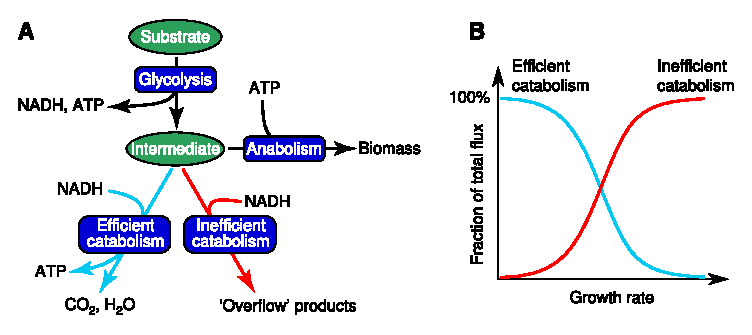
\includegraphics[width=\textwidth]{./Fig/Chapter1/molenaar_overflow.eps}
%\caption{
%\textbf{The strategy of overflow metabolism, reproduced from~\cite{molenaar_shifts_2009}.}
%When increasing the concentration of substrate, the metabolism of microorganisms switches toward the use of inefficient pathways.
%This paradoxical behavior does in fact maximize the growth rate if we take into account the costs and benefits of enzyme synthesis, in particular the fact that pathways for inefficient catabolism are shorter and therefore cheaper to produce.
%(A) Simple view of microbial metabolism, with the two competing efficient and inefficient pathways.
%(B) The switching from efficient to inefficient catabolism when the concentration of nutrients, and hence the growth rate, increases.
%}
%\label{fig:molenaar_overflow}
%\end{figure}

\subsection{Measuring growth of microorganisms}

\textbf{Either to build models or test their predictions, data on microbial growth have to be acquired.}
Measuring growth = measuring biomass accumulation, over time, and get relevant information on the cell inner state.
We have a lot of data on this.

\textbf{Measuring population-wide parameters is convenient and provides robust data.}
Population measurement is easy to implement, and some things can only be measured at the population level (so far).
But small unsynchronized effects can be hidden since we mostly work with the mean.
Despite most of the knowledge we have on microorganism growth are from population measurements, like the RNA/DNA/etc ratios, the growth laws, etc.
Extensive work of Bremmer and Dennis.
Big discoveries of the last decades that rely on population measurements ? (cite 2 or 3)

\textbf{Single-cell measurements give access to data and behaviors that are hidden at the population level.}
Single-cell measurements lay on technologies like microscopy, fluorescence, FACS...
More interesting since we can use fluorescence to not just look at the cell but also measure interesting parameters (like gene expression) at the single-cell level.
Information on the localisation of DNA, ribosomes [Bakshi].
Variability in physiology, persistors, antibiotics resistance, etc [citations]

\textbf{Batch growing conditions are convenient and close to the natural conditions of bacteria, but they raise several problems.}
Both approaches can be performed either in batch or continuous conditions.
Batch conditions is the most straight forward in lab: you put sugar in a flask, they grow until nutrient is depleted.
Implemented in flash or petri-microscopy.
Resist to contamination.
It is close to natural conditions, and industrial conditions.
Has even been used to study long-term evolution of E. coli.
But the system is poorly control, mostly because the history of the cells play a huge role in the waking process.

\textbf{Continous cultures allow to precisely control the growing conditions.}
Continuous culture consists into constantly providing nutrients to a culture, and maintaining it in a steady-state for a long time.
Implemented in bioreactor [citation] or microfluidic devices [mother machine citation].
Sensible to contaminations so hard to maintained (that's why industry ignore it so far).
Does not correspond to natural conditions but the system is fully controlled: perturbations can be applied and a lot of parameters can be monitored.
Possibility to let the cell long-enough in steady state to "forget" strain history.
Most suitable if one need to have full control on its system.

\textbf{In all these practical conditions, one can choose to either measure cells at steady-state or in dynamic.}
Finally, most of the work cited above are based on steady-state studies.
But there are also work in dynamic.
Levy showed that... in yeast.
Alon in Coli.
After decades working at steady-state, Bremmer and Dennis argued we should measure things during transitions.
de Jong / Gerosa showed that the gene expression machinery has its own dynamic that should be taken into account when measuring gene expression.
The evolutionary relevance of growth transitions has been emphasized in numerous others studies [citations lag phase, last generation before stationary, ...].

\section{Approach}
\label{sec:approach}

We first tackle the problem of creating a mathematical framework for studying environmental transitions.
\textit{Building upon the work cited above, we create a simple self-replicator model that allocate resources between two sections.}

The goal is to identify what would be an ideal transition.
\textit{We all have an intuitive idea of what should be a good transition: it should be fast, robust, etc... But it is unclear how this relates to the fitness factor that shaped the regulatory mechanisms of microorganisms.}

We describe dynamical optimality by using optimal control theory.
\textit{Brieve explanation about optimal control theory and how it is used in economic or engineering to optimize or understant dynamical processes.}

All of this is described in chapter 2.

Then, after we know what to look for, we try to actually measure how resource allocation occurs in a model organism: \textit{Escherichia coli}.
\textit{We justify the use of coli and introduce the gene expression fluorescent reporter.
We made a strain with fluorescent ribosomes, and studied our experimental framework in different transitions, at the population and the single cell level.
We justify the use of both by the fact that population is easy for "screening", and single cell allow for a better resolution and take care of the "desynchronization" biais that could occur.}

This, is described in chapter 3.

%\frontmatter
%\input{Chapters/theory_summary}
%\mainmatter
\chapter{Dynamical Allocation of Cellular Resources as an Optimal Control Problem: Novel Insights into Microbial Growth Strategies }
\chaptermark{Dynamical allocation of cell resources}
\label{chap:theory}

\textit{Rather than propose a new theory or unearth a new fact, often the most important contribution a scientist can make is to discover a new way of seeing old theories or facts.} -- Richard Dawkins, \textit{The Selfish Gene}~\cite{dawkins_selfish_1976}, preface to 1989 edition.

%\section*{Summary of chapter \thechapter}
%Microbial physiology exhibits growth laws that relate the macromolecular composition of the cell to the growth rate.
%Recent work has shown that these empirical regularities can be derived from coarse-grained models of resource allocation.
%While these studies focus on steady-state growth, such conditions are rarely found in natural habitats, where microorganisms are continually challenged by environmental fluctuations.
%The aim of this paper is to extend the study of microbial growth strategies to dynamical environments, using a self-replicator model.
%We formulate dynamical growth maximization as an optimal control problem that can be solved using Pontryagin’s Maximum Principle.
%We compare this theoretical gold standard with different possible implementations of growth control in bacterial cells.
%We find that simple control strategies enabling growth-rate maximization at steady state are suboptimal for transitions from one growth regime to another, for example when shifting bacterial cells to a medium supporting a higher growth rate.
%A near-optimal control strategy in dynamical conditions is shown to require information on several, rather than a single physiological variable.
%Interestingly, this strategy has structural analogies with the regulation of ribosomal protein synthesis by ppGpp in the enterobacterium \textit{Escherichia coli}.
%It involves sensing a mismatch between precursor and ribosome concentrations, as well as the adjustment of ribosome synthesis in a switch-like manner.
%Our results show how the capability of regulatory systems to integrate information about several physiological variables is critical for optimizing growth in a changing environment. 

\selectlanguage{french}
\section*{Résumé en français du chapître \thechapter : [titre français]}
dans cette section blablabla

\selectlanguage{english}


%%%%%% CORE OF THE ARTICLE %%%%%
\section{Introduction}

Microorganisms adapt their physiology to changes in nutrient availability in the environment.
This involves changes in the expression of a large number of genes, encoding proteins with a variety of cellular functions, such as transporters for the uptake of nutrients, enzymes for the conversion of nutrients to energy and building blocks for macromolecules, the components of the transcriptional and translational machinery, and transcription factors to preferentially direct RNA polymerase to specific promoters~\cite{schaechter_microbe_2006,keseler_ecocyc_2013}.
Fundamentally, the reorganization of gene expression in response to changes in environmental conditions is a resource allocation problem.
It poses the question how microorganisms redistribute their protein synthesis capacity over different cellular functions when constrained by the changing environment.

The mechanisms responsible for resource allocation in microbial cells are usually assumed to have been optimized through evolution, so as to maximize the offspring of cells in their natural environment.
How this general principle manifests itself on the level of cellular physiology is not straightforward though.
Many studies have reasoned that growth-rate maximization provides a selective advantage to microorganisms, because it allows competitors to be outgrown when resources are scarce.
Others have shown, however, that appropriate optimization criteria will depend on the structure of the environment and the ecosystem, as well as on the molecular properties of metabolic pathways~\cite{frank_tradeoff_2010,maclean_tragedy_2008,schuetz_multidimensional_2012,schuster_maximization_2008,schuetz_systematic_2007}.
For instance,  in environments without competition for a shared resource, maximization of growth yield rather than growth rate is expected to provide a selective advantage.
Although what counts as optimal is thus context-dependent, growth and evolution experiments in \textit{Escherichia coli} have shown that in certain conditions bacterial metabolism is indeed geared towards growth-rate maximization~\cite{edwards_silico_2001,ibarra_escherichia_2002,lewis_omic_2010}.

For this reason, growth-rate maximization is a central hypothesis in a number of recent theoretical studies of resource allocation using coarse-grained models of the cell~\cite{molenaar_shifts_2009,scott_interdependence_2010,scott_emergence_2014}.
The models deliberately reduce the molecular complexity of regulatory networks so as to focus on generic explanatory principles~\cite{servedio_not_2014}.
Along these lines, Molenaar \textit{et al.} developed a series of simple models of the microbial cell, taking into account that growth requires the synthesis of proteins playing a role in metabolism (transporters, enzymes) and gene expression (ribosomes), in varying proportions.
Allocation parameters that maximize the growth rate were shown to account, at least in a qualitative way, for the variation of the amount of ribosomal protein as a fraction of total protein in different growth media, and for the occurrence of overflow metabolism above certain growth rates~\cite{molenaar_shifts_2009}.
Using another coarse-grained model of the cell, centered on amino acid supply (metabolism) and demand (protein synthesis), Scott \textit{et al.} derived empirical growth laws with linear relations between the ribosomal protein fraction and the growth rate, in conditions where the nutrient supply or demand are altered~\cite{scott_interdependence_2010,scott_emergence_2014}.
In their model, maximization of growth rate requires maximization of amino acid flux and is achieved for a specific, unique value of the ribosomal protein fraction.
Based on a structurally similar model, Maitra and Dill related optimal resource allocation to the basic constants of the metabolic and gene expression machinery, in particular energy efficiency~\cite{maitra_bacterial_2014}.

The assumption of growth-rate maximization may lead to correct predictions in some situations, but ignores the regulatory mechanisms achieving resource allocation and therefore cannot provide a causal explanation of cellular behavior~\cite{kremling_understanding_2015}.
Several studies have used coarse-grained models to understand which control strategies microorganisms employ to achieve (optimal) resource allocation~\cite{bosdriesz_how_2015,scott_emergence_2014,weisse_mechanistic_2015}.
Scott \textit{et al.} have shown that a robust feedforward control strategy, based on the sensing of the amino acid pool size and the corresponding adjustment of the fraction of ribosomes producing ribosomal proteins, allows the ribosomal protein fraction to be maintained close to its optimal value under a variety of growth conditions~\cite{scott_emergence_2014}.
The authors suggest that this control strategy involves the signalling molecule ppGpp, in agreement with conclusions drawn from a recent kinetic model of the regulatory mechanisms achieving optimal adjustment of the ribosomal protein fraction~\cite{bosdriesz_how_2015}.
Wei{\ss}e \textit{et al.} also developed a coarse-grained model of microbial growth based on resource allocation trade-offs~\cite{weisse_mechanistic_2015}. 
Without including specific regulatory interactions, the model accounts for the above-mentioned bacterial growth laws, predicts host-circuit interactions in synthetic biology, and relates gene regulation to the nutrient composition of the medium.

The above studies consider resource allocation at steady state, where all intensive variables describing the growing microbial culture, in particular the concentrations of its molecular components, are constant (see~\cite{fishov_microbial_1995} for a precise definition of steady-state growth and the closely related notions of balanced and exponential growth).
This requires an environment to be stable over a long period of time.
Such conditions can be achieved in the laboratory~\cite{borirak_molecular_2014}, but many microorganisms naturally experience frequently-changing conditions.
For example, \textit{E. coli} can cycle between two distinct habitats, the mammalian intestine and the earth's surface (water, sediment, soil)~\cite{savageau_escherichia_1983}.
The bacteria transit through different microenvironments in the intestinal system, where they encounter different mixes of sugars~\cite{savageau_demand_1998}.
They are even more challenged in the open environment outside the host, with a greatly fluctuating availability of carbon and energy sources and a large variability in temperature, osmolarity, oxygen, and microbial communities~\cite{blount_unexhausted_2015,vanelsas_survival_2011}.

This situation motivates a dynamical perspective on microbial growth and resource allocation~\cite{pavlov_optimal_2013,vandenberg_optimal_1998,waldherr_dynamic_2015,ehrenberg_mediumdependent_2012}. However, fundamental results like the growth laws uncovered for steady-state conditions are still lacking.
In particular, extending the results reviewed above to dynamical conditions raises the following questions:
Are control strategies that maximize steady-state growth also optimal in dynamical environments?
If this is not the case, then which alternative strategies would be optimal for such conditions?
And finally, how do these strategies compare with the regulatory mechanisms that have actually evolved in microorganisms?

The aim of this study is to address the above fundamental questions in a specific dynamical growth scenario, namely a transition between two steady states following an environmental perturbation.
In particular, we consider the upshift of a microbial culture from a medium supporting growth at a low rate to a medium supporting growth at a high rate~\cite{ehrenberg_mediumdependent_2012}.
We develop a coarse-grained model of the cell, inspired by the self-replicator model of Molenaar \textit{et al.}~\cite{molenaar_shifts_2009}, and reformulate our questions in the context of optimal control theory~\cite{stengel_optimal_1994} to identify control schemes maximizing biomass production over an interval of time, the dynamical equivalent of growth-rate maximization.

We show that Pontryagin's Maximum Principle suggests that optimal resource allocation after a growth transition is achieved by a bang-bang-singular control law~\cite{stengel_optimal_1994}, a conjecture confirmed by direct numerical optimization.
This optimal solution provides a gold standard against which possible control strategies of the cell can be compared.
We consider simple strategies that drive the system to the steady state enabling growth at the maximal rate in the new medium, after the upshift.
In a dynamical growth scenario, the strategy sensing the concentration of precursor metabolites emerges as the best candidate, consistent with the analysis of Scott \textit{et al.} that feedforward activation of the rate of synthesis of ribosomal proteins, involving ppGpp-mediated sensing of the amino acid pool~\cite{dalebroux_ppgpp_2012,potrykus_pppgpp_2008,hauryliuk_recent_2015}, is the key regulatory mechanism for growth control.
It is possible, however, to define a strategy approaching the theoretical optimum even more closely by exploiting information on both the precursor concentration and the abundance of the gene expression machinery.
Interestingly, a thorough analysis of the functioning of the ppGpp system, as described by a kinetic model of the synthesis and degradation of this signalling molecule, suggests similarities between our two-variable control strategy and the regulation of the transcription of ribosomal RNA by ppGpp~\cite{bosdriesz_how_2015}.

The results presented here generalize the analysis of control strategies enabling optimal growth of microorganisms from steady-state to dynamical scenarios.
The control strategies are formulated in the context of a coarse-grained model of resource allocation, based on minimal assumptions, that accounts for empirical growth laws at steady state.
The analysis shows that during growth transitions, control strategies based on information of a single variable are outperformed by systems measuring several variables.
This conclusion agrees with the intuition that, in dynamical environments, there may be an evolutionary pressure towards more elaborate sensory systems.
From a methodological point of view, our study illustrates how optimal control theory can provide novel insights into complex biological phenomena~\cite{iglesias_control_2010}. 

%%%%%%%%%%%%%%%%%%%%%%%%%%%%%%%%%%%%%%%%%%%%%%%%%%%%%%%%%%%%%%%%%%%%%%%%%%%%%%%%%%%%%%%%%%

\section{Results}

\subsection{Self-replicator model of resource allocation}
\label{sec:model}

Resource allocation in bacteria involves the distribution of cellular resources (precursor metabolites and energy) over processes supporting maintenance and growth~\cite{schaechter_microbe_2006}.
A simple modelling tool for analyzing resource allocation questions in a precise way are so-called self-replicator models.
These models have a long history in various domains of chemistry, biology, physics, and computer science~\cite{sipper_fifty_1998}, and were recently put to use as an analytical tool in systems biology~\cite{molenaar_shifts_2009} (see also~\cite{flamm_minimal_2007}).
We will show that despite their simplicity, which make them tractable for mathematical analysis, self-replicator models are sufficiently expressive to account for empirical observations and make testable predictions.

Bearing in mind that the major constituents of the cell are macromolecules (DNA, RNA, proteins), produced from precursor metabolites, a fundamental resource allocation question is the following: How much of the cellular resources are invested in the making of new macromolecules (gene expression machinery) and how much in performing other functions, in particular producing metabolic enzymes involved in the uptake of nutrients and their conversion to precursor metabolites (metabolic machinery)?
In order to address this question, we consider a self-replicating system composed of the gene expression machinery ($R$) and the metabolic machinery ($M$).
The system, shown schematically in Fig.~\ref{fig:self_replicator}, is thus defined by two macroreactions which are conveniently written as:
\begin{equation}\label{eq:reactions}
\begin{aligned}
S &\overset{V_M}{\longrightarrow} P, \\
P &\overset{V_R}{\longrightarrow} \alpha R + (1-\alpha) M.
\end{aligned}
\end{equation}
The first reaction, catalyzed by $M$, converts external substrates ($S$) into precursor metabolites ($P$).
The second reaction, catalyzed by $R$, converts precursors into macromolecules ($R$ and $M$).
The resource allocation parameter $\alpha \in [0,1]$ defines the proportion of precursor mass used for making gene expression machinery as compared to metabolic machinery.
We will interchangeably use the symbols $M$, $R$, $S$, and $P$ for the components of the replicators themselves and their total mass [g].
We will denote the rates at which the macroreactions occur by $V_R$ and $V_M$ [g~h\textsuperscript{-1}].

\begin{figure}[tb]
\centering
\includegraphics[scale=0.7]{./Fig/Fig1}
\caption{
\textbf{Self-replicator model of bacterial growth.}
External substrates $S$ enter the cell and are transformed into precursors $P$ through the action of the metabolic machinery $M$.
The precursors are used by the gene expression machinery $R$ to make the proteins composing both the metabolic machinery (transporters, enzymes, ...) and the gene expression machinery itself (RNA polymerase, ribosomes, ...).
$\alpha$ ($1-\alpha$) is the mass proportion of precursors converted into $R$ ($M$).
Thick arrows denote reactions and thin, dashed arrows denote catalytic activities.
The rate of synthesis of precursors and the rate of synthesis of proteins from precursors are denoted by $V_M$ and $V_R$, respectively.
}
\label{fig:self_replicator}
\end{figure}

The self-replicator system in Fig.~\ref{fig:self_replicator} is based on a number of simplifying assumptions.
First, cell division is not explicitly modelled and replication should therefore be interpreted as the growth of (the mass of) a cell population.
This amounts to the assumption that individual cells in a growing populations have the same macromolecular composition.
Second, degradation of the macromolecules is ignored.
In other words, we assume that macromolecules are stable and that their degradation rates are negligible with respect to the rates of other reactions in the system.
Third, we consider only two classes of macromolecules ($R$ and $M$).
In particular, we do not assume that an irreducible mass fraction of the precursors is dedicated to cell maintenance~\cite{scott_interdependence_2010}.
The system could be easily extended to relax the above assumptions, but this would complicate the analysis of the model and obscure the points we want to make.

In what follows, it will be more convenient to describe the quantities in the system as intracellular concentrations rather than as the total mass in the cell population.
To this end, we define the volume $\mathtt{Vol}$ [L] of the cell population as follows:
\begin{equation}
\mathtt{Vol} = \beta \, (M + R),
\label{eq:voldef}
\end{equation}
with $\beta$ a conversion constant [L~g\textsuperscript{-1}] equal to the inverse of the cytoplasmic density.
Dividing each variable $M$, $R$, and $P$ by $\mathtt{Vol}$ yields the concentrations $m$, $r$, and $p$ of metabolic enzymes, ribosomes and other components of the gene expression machinery, and precursor metabolites, respectively [g~L\textsuperscript{-1}].
Henceforth, these variables as well as $\mathtt{Vol}$ and $\alpha$ will be considered functions of time $t$ [h].

The dynamics of the self-replicator in Fig.~\ref{fig:self_replicator} can be described by the following system of ordinary differential equations (see \ref{S1_Text} for the derivation):
\begin{eqnarray}
\frac{dp}{dt} &=& v_M(s,r) - v_R(p,r) \, (1+\beta\, p), \label{eq:pdef}\\
\frac{dr}{dt} &=& v_R(p,r) \, (\alpha(t) - \beta\, r), \label{eq:rdef}
\end{eqnarray}
where $s$ [g~L\textsuperscript{-1}] denote the (extracellular) concentration of substrate.
$v_M(s,r)$ [g~L\textsuperscript{-1}~h\textsuperscript{-1}] and $v_R(p,r)$ [g~L\textsuperscript{-1}~h\textsuperscript{-1}] denote the precursor synthesis rate and the macromolecule synthesis rate, respectively.
The growth rate $\mu$ [h\textsuperscript{-1}] of the replicator system is defined as the relative increase of the volume, and can be rewritten with Eqs~\ref{eq:pdef}-\ref{eq:rdef} as proportional to the macromolecule synthesis rate (\ref{S1_Text}):
\begin{equation}\label{eq:growthrate}
\mu = \frac{1}{\mathtt{Vol}} \frac{d\mathtt{Vol}}{dt} = \frac{1}{M+R}\frac{d(M+R)}{dt} = \beta\, v_R(p,r).
\end{equation}

The precursor concentration changes through the joint effect of the precursor synthesis rate $v_M(\cdot )$, the macromolecule synthesis rate $v_R(\cdot )$, and the rate of growth dilution ($\beta\, v_R(\cdot ) \,p$).
The change in concentration of ribosomes and other components of the gene expression machinery is the net effect of the ribosome synthesis rate ($\alpha (\cdot )\, v_R (\cdot)$) and the rate of growth dilution ($\beta \, v_R(\cdot) \, r $).
Remark that it is not necessary to add an equation for $m$ because it follows from Eq.~\ref{eq:voldef} that $r + m = 1/\beta$, and therefore $dm/dt = - dr/dt$.

We use Michaelis-Menten kinetics to define the synthesis rate of each reaction:
\begin{align}
v_M(s,r) &= k_M\,m\, \frac{s}{K_M + s} = k_M\,(1/\beta - r)\, \frac{s}{K_M + s},  \label{eq:metaflux} \\
v_R(p,r) &= k_R\,r\, \frac{p}{K_R + p}, \label{eq:machflux}
\end{align}
with rate constants $k_M, k_R$ [h\textsuperscript{-1}] and half-saturation constants $K_M, K_R$ [g~L\textsuperscript{-1}].
Note that the rate of precursor synthesis is proportional to the concentration of the components of the metabolic machinery, while the macromolecule synthesis rate is proportional to the concentration of the components of the gene expression machinery.
These catalytic effects correspond to the dashed arrows in Fig.~\ref{fig:self_replicator}.
The rate constant $k_M$ depends both on the quality of the nutrients in the medium (higher $k_M$ for a richer medium) and on the metabolic efficiency of the macroreaction converting the substrate into precursors (higher $k_M$ for a more efficient reaction).
For convenience, we henceforth assume that the environmental conditions do not change over the time-interval considered, either because $s$ is constant or because $s \gg K_M$, corresponding to a situation in which the substrate is available in excess.
In both cases, $e_M(s) = k_M\, s/(K_M + s)$ is approximately constant, so that we can write
\begin{equation}
\label{eq:metaflux_simplified}
v_M (r) = e_M \, (1/\beta-r).
\end{equation}
The rate constant $k_R$ characterizes the efficiency of the gene expression machinery, depending on the elongation rate of ribosomes, among other things. The ratio $p/K_R$ is an indicator of the saturation of the gene expression machinery by precursors.

The system of Eqs~\ref{eq:pdef}-\ref{eq:rdef} thus has four parameters ($e_M$, $k_R$, $K_R$, $\beta$), one of which characterizes the input from the environment ($e_M$).
The order of magnitude of the parameters can be inferred from data in the literature, as explained in \ref{S2_Text}.
Below we use the following values for the parameters $e_M = 3.6$~h\textsuperscript{-1}, $k_R = 3.6$~h\textsuperscript{-1}, $K_R=1$~g~L\textsuperscript{-1}, $\beta = 0.003$~L~g\textsuperscript{-1} (\ref{S1_Table}).
However, it should be emphasized that the conclusions of this paper do not depend on the exact quantitative values of these parameters.

An interesting property of the model is that it is built on minimal assumptions, basically the two macroreactions and the definition of the volume as proportional to the total mass of macromolecules.
Like in~\cite{molenaar_shifts_2009,pavlov_optimal_2013,scott_emergence_2014}, these assumptions directly lead to the expression of the growth rate in Eq.~\ref{eq:growthrate}, without additional assumptions.

\subsection{Growth-rate maximization of the self-replicator reproduces bacterial growth laws}
\label{sec:growthlaws}

The nullcline for $r$ is given by $r=0$, $r=\alpha/\beta$, and $p=0$, while the nullcline for $p$ is defined by

\[
r = \frac{e_M}{\beta \left(e_M + k_R\, \frac{p}{K_R+p}\, (1+\beta p)\right)}.
\]
The nullclines define a single stable steady state $(p^*, r^*)$ (Fig.~\ref{fig:model_analysis}\textit{A} and \textit{Methods}).
At this steady state, the growth rate is constant and denoted by $\mu^*$.
The nullcline for $p$ is defined by the environment $e_M$.
The nullcline for $r$, and thus the location of the steady state with the associated growth rate, are given by $\alpha$.
Fig.~\ref{fig:model_analysis}\textit{B} shows the dependency of the steady-state growth rate $\mu^*$ on the resource allocation parameter $\alpha$.
As can be seen, $\mu^*$ is maximal for a specific, unique value of $\alpha$, which we denote $\alpha_{opt}^*$.
That is, the model predicts that there is a single optimal way to divide the precursor flux over the synthesis of the gene expression machinery and the metabolic machinery.
The same result, using a similar model, was obtained by Scott \textit{et al.}~\cite{scott_emergence_2014}.
The self-replicator model is simple enough to derive an algebraic expression for computing $\alpha^*_{opt}$ and the corresponding maximal growth rate $\mu^*_{opt}$ (\textit{Methods} and \ref{S1_Text}), which will simplify analysis of the system in later sections.

\begin{figure}[tb]
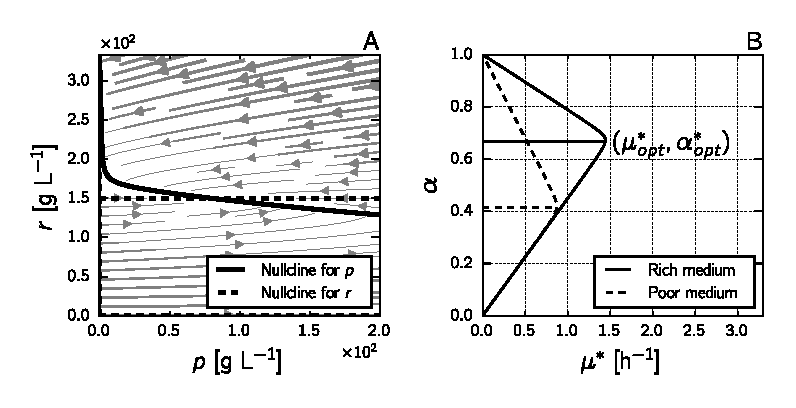
\includegraphics[width=\textwidth]{./Fig/Fig2}
\caption{\textbf{Analysis of self-replicator model of bacterial growth.}
\textit{A:}~Phase-plane analysis of the self-replicator model of Eqs~\ref{eq:pdef} and \ref{eq:rdef}.
The nullclines for $p$ and $r$ are shown as solid and dashed curves, respectively.
Parameter values are $e_M = 3.6$~h\textsuperscript{-1}, $k_R = 3.6$~h\textsuperscript{-1}, $K_R=1$~g~L\textsuperscript{-1}, $\beta = 0.003$~L~g\textsuperscript{-1}, $\alpha = 0.45$.
\textit{B:}~Dependence of the growth rate at steady state $\mu^{*}$ on the resource allocation parameter $\alpha$, for two different environmental conditions (solid line, $e_M = 4.76$~h\textsuperscript{-1}; dashed line, $e_M = 1.57$~h\textsuperscript{-1}, other parameter values are $k_R = 2.23$~h\textsuperscript{-1}, $K_R=1$~g~L\textsuperscript{-1}, and $\beta = 0.003$~L~g\textsuperscript{-1}).
The maximal growth rate is attained for a unique $\alpha$, called $\alpha^*_{opt}$.
}
\label{fig:model_analysis}
\end{figure}

In order to validate the model, we verified that it can account for data on the macromolecular composition of \textit{E. coli} at steady state~\cite{scott_interdependence_2010}.
When optimizing $\alpha$ for different values of $e_M$ (assuming cells attain maximal growth), the model predicts a relation between $\alpha^*_{opt}$ and $\mu^*_{opt}$ (colored dots and black dashed line in Fig.~\ref{fig:model_validation}\textit{A}) that is quasi-linear for high growth rates.
We compared this prediction with the results of experiments where the relation between the growth rate and the mass ratio of total RNA and protein was determined in different growth media (Fig.~\ref{fig:model_validation}\textit{B}).
In the framework of our model, different media correspond to different values of $e_M$, and different total RNA/protein mass ratios to different values of $\alpha$ (up to a conversion factor), allowing a direct comparison of the model predictions in Fig.~\ref{fig:model_validation}\textit{A} with the data in Fig.~\ref{fig:model_validation}\textit{B} (see \textit{Methods}).
As can be seen, the model is able to account for the observed quasi-linear relation between the growth rate and the total mass ratio of RNA and protein. 
Moreover, for realistic values of $k_R$ and $e_M$, a good quantitative fit is obtained (\textit{Methods} and \ref{S1_Table}).

\begin{figure}[p]
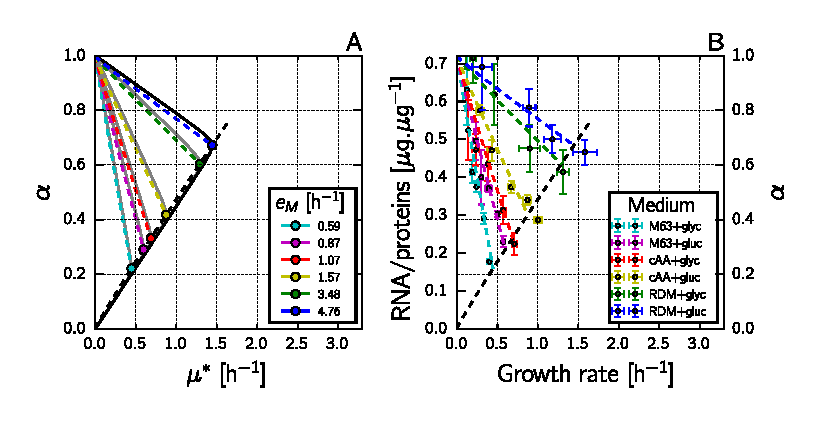
\includegraphics[width=\textwidth]{./Fig/Fig3}
\caption{
\textbf{Self-replicator model accounts for bacterial growth laws.}
\textit{A:}~Predicted quasi-linear relation between the maximal growth rate $\mu^{*}_{opt}$ and the corresponding optimal resource allocation $\alpha^*_{opt}$, for different values of $e_M$ (different colors).
The colored dots indicate $\alpha^*_{opt}$ and $\mu^{*}_{opt}$  for $k_R = 2.23$~h\textsuperscript{-1} and different $e_M$, and the dashed black line the relation for all intermediate values of $e_M$.
The dashed colored lines indicate the relation between $\alpha^*_{opt}$ and $\mu^{*}_{opt}$ obtained when, for a given value of $e_M$, the value of $k_R$ is decreased (lower $k_R$ leads to lower $\mu^{*}_{opt}$).
The solid grey curves correspond to $(\mu^*,\alpha)$-profiles like those shown in Fig.~\ref{fig:model_analysis}\textit{B}.
\textit{B:}~Measured relation between the total RNA/protein mass ratio and the growth rate, in different growth media with different doses of a translation inhibitor (data from~\cite{scott_interdependence_2010}).
For each medium, indicated by a color, five different concentrations of inhibitor were used (higher dose leads to lower growth rate).
Growth-medium compositions are given in the original publication and error bars represent standard deviations.
The dashed black and colored lines are the same as in panel \textit{A}, indicating the good quantitative correspondence between model predictions and experimental data for the chosen parameter values, obtained by fitting the model to the data points (see \textit{Methods} for details).
}
\label{fig:model_validation}
\end{figure}

The data from Scott \textit{et al.} also reveal a second apparently linear relation between the growth rate and the total RNA/protein mass ratio.
This relation is obtained when varying, in the same growth medium, the efficiency of protein synthesis by adding different doses of an inhibitor of translation (chloramphenicol)~\cite{scott_interdependence_2010}.
Using the model, we computed $\alpha^*_{opt}$ and $\mu^*_{opt}$, for constant environment $e_M$ and different values of the efficiency of protein synthesis $k_R$ (dashed colored lines in Fig.~\ref{fig:model_validation}\textit{A}).
As can be seen in Fig.~\ref{fig:model_validation}\textit{B}, the model also captures the second linear relation in the data.

We conclude that the self-replicator model is able to reproduce known observations of resource allocation in bacteria, so-called growth laws~\cite{scott_interdependence_2010}.
The model is similar to a model recently proposed by Scott \textit{et al.}~\cite{scott_emergence_2014}.
Contrary to the latter model, the translation rate is not assumed to be constant in the self-replicator model, but rather depends on precursor abundance, as proposed by the same authors in~\cite{klumpp_molecular_2013}.

The above analysis of bacterial growth has two major limitations.
First, the predictions of optimal resource allocation (the value of $\alpha$ leading to the maximal growth rate) hold at steady state, for a constant environment, whereas most bacteria are not expected to encounter such conditions outside the laboratory.
An allocation of resources that is optimal for steady-state growth and constant over time may not be optimal in dynamical growth conditions.
Second, while it predicts which value of $\alpha$ is optimal at steady state, the model says nothing about the strategies that could be used to control resource allocation and set $\alpha$ to its optimal value.
In other words, how could bacterial cells use sensors of changes in their internal state and the environment to optimally adjust $\alpha$?
In what follows, we will address the above two questions, after having given a precise statement of the problem of optimal resource allocation in a dynamical environment in the next section. 

\subsection{Biomass maximization as an optimal control problem}
\label{sec:optimalcontrolproblem}

A self-replicator at steady state accumulates biomass according to \\ $\texttt{Vol}(0)\, e^{\mu^*\, t}$, $t\in [0,\tau]$, when $\mu^*$ is the growth rate at steady state. 
The accumulation of biomass is obviously maximal when the growth rate is maximal ($\mu^* = \mu^*_{opt}$).
In dynamical conditions, the growth rate is not constant and biomass accumulation is described more generally by: 
\begin{equation*}
\frac{d\texttt{Vol}}{dt} = \mu(t) \, \texttt{Vol}.
\end{equation*}
In other words, when integrating over the time interval $[0,\tau]$:
\begin{equation}\label{eq:biomassdyn}
\ln \left(\frac{\texttt{Vol}(\tau)}{\texttt{Vol}(0)}\right) =  \int_{0}^{\tau} \mu(t) \, dt.
\end{equation}
Since the logarithm is an increasing function, maximizing the biomass produced over $[0,\tau]$ requires maximization of the right-hand side of the equation.

In a changing environment, maximization of the integral in Eq.~\ref{eq:biomassdyn} will generally require the optimal value of $\alpha$ to be a function of time instead of a specific constant value.
This dynamical resource allocation problem can be formulated in a more precise way using concepts from optimal control theory~\cite{stengel_optimal_1994}. 
Let $J$ be the objective function  
\begin{equation*}
J(\alpha)= \int_{0}^{\tau} \mu(t) \, dt = \int_{0}^{\tau} \beta \, v_R(p,r) \, dt,
\end{equation*}
where $\alpha:\mathbb{R}^+ \rightarrow [0,1]$ is a time-dependent function. 
The time evolution of $p$ and $r$ is determined by the self-replicator model of Eqs~\ref{eq:pdef} and \ref{eq:rdef}, and $p$ and $r$ thus depend on $e_M$ and $\alpha$. 
Moreover, let $\mathcal{U}=\{\alpha:\mathbb{R}^+ \rightarrow [0,1] \}$ be the set of admissible controls. 
The optimal dynamical control problem then consists in finding the time-varying function $\alpha_{opt}(t)$ that maximizes $J(\alpha)$ over the time-interval $[0,\tau]$:

\begin{equation}
\alpha_{opt} = \arg \underset{\alpha \in \mathcal{U}}{\max} \ J(\alpha).
\label{eq:J}
\end{equation}

In what follows, we will simplify the above problem by considering that the environment changes in a step-wise fashion at $t=0$, but remains constant over the time-interval $[0,\tau]$, that is, $e_M(t)=e_M$.
More specifically, we focus on the case of a nutrient upshift, corresponding to a step-wise increase of $e_M$.
This upshift scenario corresponds to classical experiments in bacterial physiology~\cite{kjeldgaard_kinetics_1961,schaechter_patterns_1961,johnsen_control_1977}, reviewed in~\cite{ehrenberg_mediumdependent_2012}, and is frequently encountered in the life cycle of a microorganism~\cite{schaechter_microbe_2006}.
Notice that more complex environments can be approximated by a sequence of step-wise nutrient upshifts and downshifts.

\subsection{Solution of the optimal control problem}
\label{sec:optimalcontrolsolution}

Optimal dynamical control problems for two-dimensional nonlinear dynamical systems, like the problem of Eq.~\ref{eq:J}, are generally difficult to solve.
However, we will show that the class of functions to which $\alpha_{opt}$ belongs can be identified, and we will use numerical optimization to identify a particular $\alpha_{opt}$ maximizing $J$.

As a preliminary step, in order to simplify the analysis, the variables in the self-replicator model of Eqs~\ref{eq:pdef} and \ref{eq:rdef} are made nondimensional, by defining $\hat{t} = k_R\, t$, $\hat{p} = \beta\, p$, and $\hat{r} = \beta\, r$.
This leads to the following ODE system:
\begin{eqnarray}
\frac{d\hat{p}}{d\hat{t}} &=& (1-\hat{r})\, E_M - (1+\hat{p})\, \hat{r} \, \frac{\hat{p}}{K+\hat{p}}, \label{eq:pdefnondim}\\
\frac{d\hat{r}}{d\hat{t}} &=& \hat{r} \frac{\hat{p}}{K + \hat{p}} \, (\alpha (\hat{t}) - \hat{r}), \label{eq:rdefnondim}
\end{eqnarray}
where $K= \beta\, K_R$ and $E_M= e_M / k_R$.
The nondimensional growth rate is given by:
\begin{equation}
\label{eq:munondim}
\hat{\mu} = \frac{\mu}{k_R} = \frac{\hat{p}}{K + \hat{p}} \, \hat{r} .
\end{equation}
Notice that the nondimensionalized system depends on a single parameter $K$, in addition to the constant environment $E_M$, which functions as an input to the system.

Analysis of the nondimensionalized system allows a number of properties of the solution of the optimal control problem of Eq.~\ref{eq:J} to be derived (\textit{Methods} and \ref{S3_Text}).
First, by applying a version of the well-known Pontryagin Maximum Principlek~\cite{carlson_infinite_1991}, we can prove that the optimal solution is obtained for an alternating sequence of $\alpha(\cdot)=0$ and $\alpha(\cdot)=1$, possibly ending with an intermediate value of $\alpha(\cdot)$, corresponding to the optimal steady state $(\hat{p}(t),\hat{r}(t))=(\hat{p}_{opt}^*,\hat{r}_{opt}^*)$, that is, the steady state leading to the optimal growth rate $\hat{\mu}_{opt}^*$ in the post-upshift environment $E_M$.
Second, if the optimal solution reaches the optimal steady state for the new environment, then it does so after an infinite number of switches of $\alpha (\cdot)$ between 0 and 1.
Third, this switching behavior is characterized by a so-called switching curve $\hat{r}=\varphi(\hat{p})$ in the $(\hat{p},\hat{r})$-plane, which passes through $(\hat{p}_{opt}^*,\hat{r}_{opt}^*)$.
The switching curve divides the phase plane into two regions, such that $\alpha(\cdot)$ switches to 0 when the system is in the region above $\varphi$ and to 1 when the system is below $\varphi$ (black dashed curve in Fig.~\ref{fig:optimalcontrol}\textit{A}).

\begin{figure}[tb]
\centering
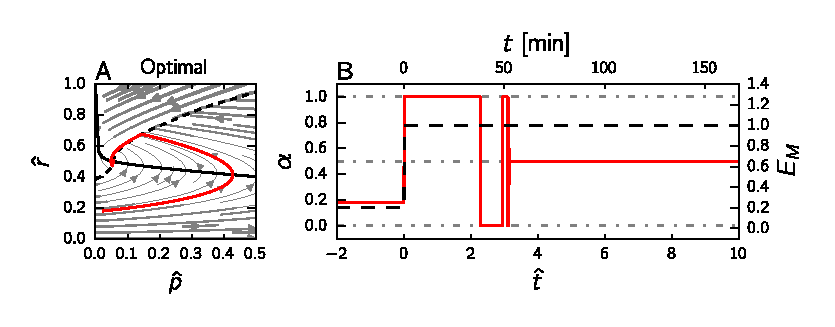
\includegraphics[width=\textwidth]{./Fig/Fig4}
\caption{
\textbf{Optimal control of the self-replicator during a nutrient upshift.}
\textit{A:}~Optimal trajectory in the phase plane for the nondimensionalized model of Eqs~\ref{eq:pdefnondim}-\ref{eq:rdefnondim}, with streamlines. The optimal trajectory is shown as a solid, red curve.
The solid, black curve represents the $\hat{p}$-nullcline.
The dashed, black curve is the switching curve $\varphi(\hat{p})$.
The optimal solution was obtained by numerical optimization using \texttt{bocop}~\cite{bonnans_bocop_2012} (see \textit{Methods} for details), using the parameter values $E_M=1$ and $K=0.003$, and starting from the initial state $(0.024,0.18)$ at $t=0$ (optimal steady state for $E_M=0.2$).
\textit{B:}~Time evolution of the control variable $\alpha_{opt}(\cdot)$ (thick, red line) and the environment $E_M$ (dashed, black line).
}
\label{fig:optimalcontrol}
\end{figure}

In line with these results, we conjecture that the optimal solution consists in a switching transient towards the optimal steady state for the new environment, and remains at this steady state until the next environmental change.
Such a solution is known as a bang-bang-singular solution in the control theory literature~\cite{stengel_optimal_1994}.
Formally, the solution of Eq.~\ref{eq:J} can be described as
\begin{equation}
\label{eq:optcontrol}
\alpha_{opt}(\hat{t})=
\begin{cases}
0, \ \textrm{if} \ \hat{r}(\hat{t}) > \varphi(\hat{p}(\hat{t})),\\
1, \ \textrm{if} \ \hat{r}(\hat{t}) < \varphi(\hat{p}(\hat{t})), \\
\alpha^*_{opt}, \ \textrm{if} \ (\hat{p}(\hat{t}),\hat{r}(\hat{t}))=(\hat{p}_{opt}^*,\hat{r}_{opt}^*).
\end{cases}
\end{equation}
Notice that the optimal solution involves dynamical feedback from the state of the system to the control variable $\alpha(\cdot)$, and is therefore an instance of closed-loop optimization~\cite{stengel_optimal_1994}.

The optimal control problem of Eq.~\ref{eq:J} was also solved numerically by a direct method using the \texttt{bocop} software~\cite{bonnans_bocop_2012} (see \textit{Methods} for details).
A time discretization allows the problem to be transformed into a nonlinear optimization problem solved here by interior point techniques.
The optimal trajectories obtained numerically confirm our conjecture that the optimal control is bang-bang-singular.
An example solution, obtained by numerical optimization is shown in Fig.~\ref{fig:optimalcontrol}.
At time $\hat{t}=0$, $E_M$ jumps from a low to a high value, corresponding to a nutrient upshift (dashed black line in Fig.~\ref{fig:optimalcontrol}B).
The optimal solution $\alpha_{opt}$ consists of a sequence of switches between $\alpha=1$, corresponding to maximal synthesis of the gene expression machinery, and $\alpha=0$, corresponding to maximal synthesis of the metabolic machinery, until $(\hat{p}_{opt}^*,\hat{r}_{opt}^*)$ is reached.
$\alpha$ is then set to $\alpha^*_{opt}$, the value leading to the maximum growth rate in the new medium (here 0.5, for $E_M=1$).
The sequence of switches of $\alpha$ in Fig.~\ref{fig:optimalcontrol}\textit{B} corresponds to successive crossings of the switching curve in Fig.~\ref{fig:optimalcontrol}\textit{A}.
In particular, the switch just after $\hat{t}=2$ corresponds to the first crossing of the switching curve; the subsequent switches accumulate around the steady state and are therefore difficult to identify in the plot.

What is the biological relevance of the bang-bang-singular solution maximizing growth of the bacterial self-replicator?
In order to answer this question, we will investigate in the next two sections the different ways in which microorganisms could implement or have been shown to implement feedback growth control by sensing the environment and cellular physiology.
Although the idealized solution proposed by optimal control theory will obviously not be found in nature, actual control strategies may produce solutions that are close.
The optimal solution can thus be used as a gold standard, a benchmark for comparing actual control strategies. 

\subsection{Simple feedback control strategies: exploiting information on nutrients or precursors}
\label{sec:steadystate}

The control strategies that microbial cells have evolved to bring resource allocation in line with changes in the environment involve a variety of molecular mechanisms~\cite{chubukov_coordination_2014}.
These mechanisms are responsible for sensing the environment and the physiological state of the cell, as well as for adjusting the expression of genes that encode components of the transcriptional and translational machinery, enzymes, transporters, and proteins with other metabolic functions.

In the framework of the self-replicator model of bacterial growth, control strategies take the form of feedback control laws mapping the value of system variables to a value of the control variable $\alpha(\cdot)$.
In this section, we explore two such strategies, the first exploiting information on the quality and quantity of substrate present in the environment, as reflected in the value of $E_M$, and the second using information on the precursor concentration $\hat{p}$.
The feedback control strategies are graphically displayed in Fig.~\ref{fig:strategies_overview}, as an extension of the self-replicator of Fig.~\ref{fig:self_replicator}.
We pose a number of mathematical constraints on the feedback control strategies considered below.
First, we require the control laws to be functions of the variables of the self-replicator but not involve derivatives or integrals of these variables.
Second, for a constant environment $E_M$, the control strategies must drive the system to a unique stable and non-trivial steady state, enabling a non-zero growth rate.
Third, this steady state must equal the optimal steady state for that environment, given by $(\hat{p}_{opt}^*,\hat{r}_{opt}^*)$.


\begin{figure}[tb]
\centering
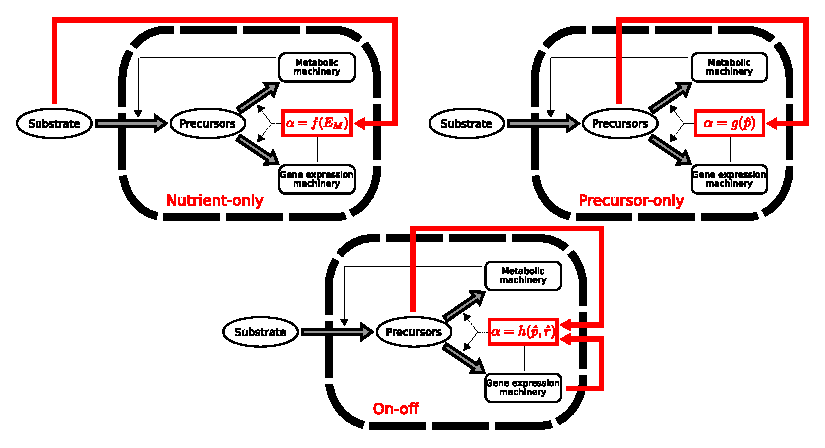
\includegraphics[width=\textwidth]{./Fig/Fig5}
\caption{
\textbf{Alternative strategies for controlling the self-replicator of bacterial growth.}
The feedback control strategies, shown in red and superposed on the self-replicator of Fig.~\ref{fig:self_replicator}, exploit information on system variables and the environment to adjust the value of $\alpha$, and thus the relative allocation of resources to the metabolic machinery and gene expression machinery.
}
\label{fig:strategies_overview}
\end{figure}


The first control strategy is defined by the function $f \colon \mathbb{R}^+ \to [0,1]$, mapping $E_M$ to $\alpha$:
\begin{equation}
\alpha = f(E_M).
\label{eq:f}
\end{equation}
Notice that $\alpha$ is constant because $E_M$ is fixed to the value defining the new environment after the upshift.
What would be an appropriate choice for $f$?
An advantage of the self-replicator model is that the optimal allocation at steady state can be explicitly formulated as a function of $E_M$ (Eq.~\ref{eq:alpha_mu_optimal} in \textit{Methods}, with derivation in \ref{S1_Text}).
This function is the unique function satisfying all of the above criteria (\ref{S1_Text}).
\ref{S1_Fig} plots $f$ and shows that it is conveniently approximated by a Michaelis-Menten function, \textit{i.e.},
\begin{equation}\label{eq:MMApprox}
\alpha(\cdot) = \dfrac{E_M}{E_M + K_{mE}},
\end{equation}
with the dimensionless half-saturation constant $K_{mE}$.
The interest of the approximation is that it demonstrates that the control strategy can be described by a simple and ubiquitous response curve in biochemical kinetics.
 
As an example of a regulatory system resembling the above control strategy consider the phosphotransferase system responsible for the uptake of glucose, the preferred substrate of \textit{E. coli}~\cite{deutscher_how_2006}.
In the presence of glucose, the EIIA\textsuperscript{Glc} component of the phosphotransferase system is mostly unphosphorylated, since the phosphate groups are used for the conversion of extracellular glucose to intracellular glucose-6-phosphate.
When glucose disappears from the medium, however, the glucose uptake rate decreases and, correspondingly, the phosphorylated fraction of EIIA\textsuperscript{\textrm{Glc}} increases.
The phosphorylation state of EIIA\textsuperscript{\textrm{Glc}} thus provides an indirect read-out of glucose availability.
In response to this signal, a variety of metabolic processes are upregulated or downregulated, notably involving the signalling molecule cAMP which activates the pleiotropic transcription factor Crp~\cite{deutscher_how_2006,gorke_carbon_2008}.

How does the control strategy of Eq.~\ref{eq:f}, which we call a nutrient-only strategy, perform in comparison with the optimal solution derived in the previous section?
That is, how much biomass does this strategy produce compared with the maximal amount of biomass that can theoretically be obtained after a nutrient upshift?
In order to answer these questions, we simulated the response to a sudden upshift of the self-replicator of Eqs~\ref{eq:pdefnondim}-\ref{eq:rdefnondim} controlled by the nutrient-only strategy of Eq.~\ref{eq:f}.
The results are shown in Fig.~\ref{fig:comparison_nutrients_precursor}.
Panel~\textit{A} shows the trajectory of the controlled self-replicator system and panel~\textit{D} plots the evolution of the amount of biomass as a fraction of the amount of biomass produced by the optimal strategy.
While the system does reach the steady state that is optimal for $E_M$, the nutrient-only strategy has poor performance in the transient phase immediately following the nutrient upshift.
As can be seen from the solution trajectory in Fig.~\ref{fig:comparison_nutrients_precursor}\textit{A}, fixing $\alpha$ to the value that enables optimal growth at steady state leads to a huge transient overshoot of the precursor concentration.
The overshoot reveals that resource allocation is initially suboptimal, with too many resources invested in the metabolic machinery at the expense of the gene expression machinery.
This causes a transiently suboptimal growth rate, leading to lower biomass accumulation (Eq.~\ref{eq:biomassdyn}).

\begin{figure}[p]
\centering
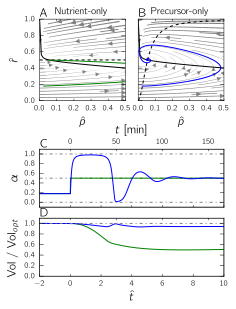
\includegraphics[scale=1]{./Fig/Fig6}
\caption{
\textbf{Comparison of the performance of the nutrient-only and precursor-only strategies after a nutrient upshift.}
\textit{A:}~Trajectory in the phase plane for the nutrient-only strategy (green curve).
The solid, black curve represents the $\hat{p}$-nullcline.
The dashed, black curve is the $\hat{r}$-nullcline.
The solution is obtained by numerical simulation of the system of Eqs~\ref{eq:pdefnondim}-\ref{eq:rdefnondim}, supplemented with $\alpha = f(E_M)$ as specified by Eq.~\ref{eq:meth_f} in the \textit{Methods} section and plotted in \ref{S1_Fig}.
The initial state corresponds to the steady state attained for an environment given by $0.2 \, E_M$.
While converging to the new steady state after the upshift, the precursor concentration makes a large overshoot.
\textit{B:}~As above, but for the precursor-only strategy.
The feedback control strategy is now defined by $\alpha = g(\hat{p})$ as specified by Eq.~\ref{eq:meth_g} in the \textit{Methods} section and plotted in \ref{S1_Fig}.
The solution trajectory (blue curve) exhibits a lower overshoot.
\textit{C:}~Evolution of the control variable $\alpha(\cdot)$ as a function of time, for each of the above two strategies.
Notice that in the nutrient-only strategy $\alpha(\cdot)$ immediately jumps to the optimal value for the post-upshift steady state (green curve), whereas in the precursor-only strategy it depends on the (time-varying) precursor concentration (blue curve).
\textit{D:}~Evolution of the ratio $\texttt{Vol} / \texttt{Vol}_{opt}$  as a function of time, where $\texttt{Vol}$ is the volume of the self-replicator and $\texttt{Vol}_{opt}$ the volume of the same replicator following the optimal strategy shown in Fig.~\ref{fig:optimalcontrol}.
In all of the above simulations, the parameter values $E_M=1$ and $K=0.003$ were used.
}
\label{fig:comparison_nutrients_precursor}
\end{figure}

One way to avoid the transient precursor imbalance observed in Fig.~\ref{fig:comparison_nutrients_precursor}\textit{A} would be to exploit information on the precursor concentration in the control strategy.
The second strategy considered here, which we label a precursor-only strategy, does exactly this: it involves a feedback control law $g \colon \mathbb{R}^+ \to [0,1]$ mapping $\hat{p}$ to $\alpha$:

\begin{equation}
\alpha = g(\hat{p}).
\label{eq:precursorstrategy}
\end{equation}
Since $\hat{p}$ will vary during the upshift experiment, $\alpha$ is not constant, contrary to the nutrient-only strategy above.
In the \textit{Methods} section, we present a function $g$ satisfying the requirements listed in the beginning of this section, in particular that the system converge to a stable steady state ensuring maximal growth in the new environment.
Moreover, we show that any other choice for $g$ leads to lower biomass production.
The function is plotted in \ref{S1_Fig}, and as shown in the same panel, is conveniently approximated by a Hill function with cooperativity coefficient 2:
\begin{equation}\label{eq:HillApprox}
\alpha (\cdot)= \dfrac{\hat{p}^2}{\hat{p}^2 + {K_{mp}}^2},
\end{equation}
where $K_{mp}$ is a dimensionless half-saturation constant.

While converging to the same steady state, this second strategy, which we will refer to as the precursor-only strategy, performs much better than the nutrient-only strategy after an upshift, as shown in Fig.~\ref{fig:comparison_nutrients_precursor}.
We simulated the response to a nutrient upshift of the self-replicator of Eqs~\ref{eq:pdefnondim}-\ref{eq:rdefnondim} with the precursor-only strategy of Eq.~\ref{eq:precursorstrategy}.
The relative biomass increases by 51\% and reaches 94\% of the biomass produced by the optimal control strategy (the theoretical maximum).
The precursor-only strategy notably avoids the inefficient transient accumulation of precursors directly after the nutrient upshift, by alternatingly investing more resources in gene expression (consumption of precursors) and metabolism (production of precursors).
In this respect, the oscillatory time profile of $\alpha$ (Fig.~\ref{fig:comparison_nutrients_precursor}\textit{C}) is somewhat reminiscent of the bang-bang-singular control in the solution of the optimal control problem (Fig.~\ref{fig:optimalcontrol}\textit{B}).

Both strategies, nutrient-only and precursor-only, drive the self-replicator towards the same steady state.
Whereas the two strategies are thus indistinguishable when the analysis is restricted to steady state, the precursor-only strategy is shown to perform much better in a dynamical upshift scenario, in the sense that the biomass produced is much closer to that produced by the optimal strategy.
Several authors have concluded that control strategies based on precursor sensing are key for maintaining optimal growth at steady state.
Scott \textit{et al.} argue that a strategy similar to the precursor-only approach above allows robust control of amino acid supply and demand, resulting in optimal steady-state growth over a range of nutrient conditions~\cite{scott_emergence_2014}.
They associate this strategy with ppGpp-mediated control of the synthesis of ribosomal proteins~\cite{dalebroux_ppgpp_2012,potrykus_pppgpp_2008,hauryliuk_recent_2015}.
The signalling molecule ppGpp accumulates in response to an increase in the level of uncharged tRNA, when amino acid concentrations in the cell drop. 
This causes ribosomes to "stall" and leads to RelA-mediated conversion of GTP to ppGpp, the molecular details of which are still subject of debate~\cite{english_singlemolecule_2011,hauryliuk_recent_2015}.
Since ppGpp inhibits the transcription of ribosomal RNAs~\cite{dennis_control_2004}, the concentration of the latter decreases, leading to more inactive ribosomal proteins and, through a well-characterized post-transcriptional autoregulatory mechanism, a lower synthesis rate of ribosomal proteins~\cite{keener_regulation_1996,potrykus_pppgpp_2008}.
Our analysis adds to the above study a novel insight: measuring precursors does not only enable resource allocation control to achieve maximal growth at steady state, but is also a good strategy in a dynamical context.

While the precursor-only strategy is thus seen to lead to good results, Fig.~\ref{fig:comparison_nutrients_precursor}\textit{D} shows that there remains room for improvement.
It seems reasonable to expect that control strategies exploiting information of not just a single variable, but several variables simultaneously, could further improve the performance of the self-replicator during a growth transition.


\subsection{A near-optimal feedback control strategy: exploiting information on the imbalance between precursors and the gene expression machinery}
\label{sec:strategies}

In the quest for further improvements, a natural starting-point would be to consider the curve defining the optimal steady states $(\hat{p}^*_{opt},\hat{r}^*_{opt})$  for different environments $E_M$.
This curve is defined by a function mapping $\hat{p}^*$ to $\hat{r}^*$, which is actually the same as the function $g$ introduced in the precursor-only strategy (\textit{Methods} and \ref{S1_Fig}), given that at steady state $\hat{r}=\alpha$ (Eq.~\ref{eq:rdefnondim}).
The curve can be seen as representing an optimal balance between precursors and the gene expression machinery, in the sense that the maximal growth rate attainable for a given precursor concentration $\hat{p}$ requires a concentration $\hat{r}$ of ribosomes and other components of the gene expression machinery equal to $g(\hat{p})$. 
If either $\hat{r}>g(\hat{p})$ or $\hat{r}<g(\hat{p})$, the growth rate is suboptimal.

These considerations suggest an intuitive control strategy, namely to avoid an imbalance between $\hat{p}$ and $\hat{r}$ at all times, and remain as close as possible to the curve defined by $g$.
In particular, when the gene expression machinery is more abundant than what is optimal given the available precursors ($\hat{r} > g(\hat{p})$), its synthesis is switched off ($\alpha = 0$).
Conversely, when $\hat{r} < g(\hat{p})$, synthesis of the gene expression machinery is switched on.
This strategy thus tries to restore "as quickly as possible" the optimal balance between precursors $\hat{p}$ and the gene expression machinery $\hat{r}$, giving rise to a so-called on-off control strategy:
\begin{equation}
\label{eq:stratswitch}
\alpha = h(\hat{p},\hat{r}) =
\begin{cases}
0, \ \textrm{if} \ \hat{r} > g(\hat{p}),\\
1, \ \textrm{if} \ \hat{r} < g(\hat{p}), \\
\alpha_{opt}^* \ \textrm{if} \ (\hat{p},\hat{r})=(\hat{p}_{opt}^*,\hat{r}_{opt}^*).
\end{cases}
\end{equation}

As shown in the \textit{Methods} section, the on-off strategy drives the system to a stable steady state ensuring growth at the maximal rate.
Notice that, contrary to the strategies discussed in the previous section, the value of $\alpha$ selected by the on-off strategy depends on both $\hat{p}$ and $\hat{r}$ (Fig.~\ref{fig:strategies_overview}).
It thus uses more information on the state of the system than the nutrient-only and precursor-only strategies.

Fig.~\ref{fig:onoffresults} shows the performance of the on-off strategy after a nutrient upshift, as compared to the precursor-only strategy.
The transition is seen to be nearly perfect, in the sense that 98\% of the optimal biomass is produced by the strategy.
The time course of $\alpha$ in panel \textit{D} is very similar to the optimal time course obtained by numerical optimization, shown in Fig.~\ref{fig:optimalcontrol}\textit{B}, and clearly brings out the bang-bang-singular nature of the solution. 
These results show that a strategy exploiting complete information on the internal state of the self-replicator can lead to near-optimal performance, outcompeting a strategy that uses partial information on the internal state (precursor abundance only).

\begin{figure}[p]
\centering
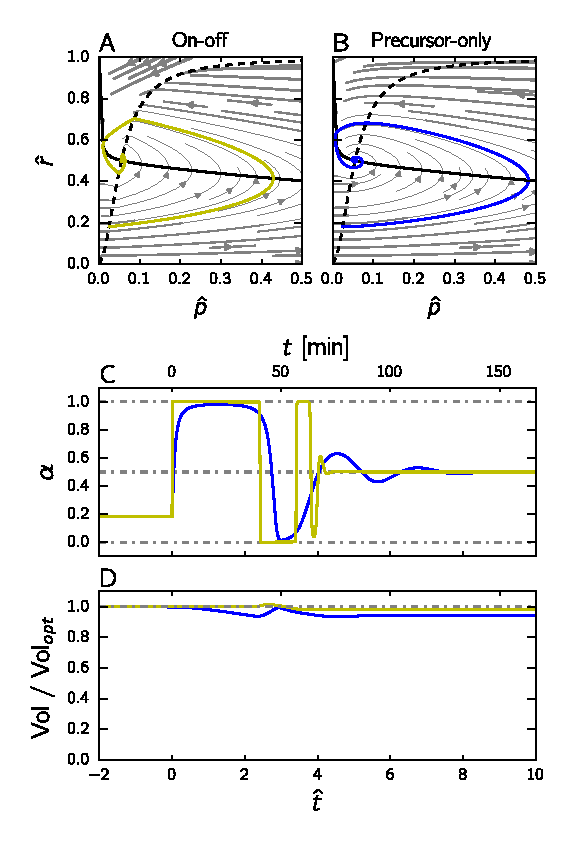
\includegraphics[scale=1]{./Fig/Fig7}
\caption{
\textbf{Comparison of the performance of the precursor-only and the on-off strategies after a nutrient upshift.}
\textit{A:}~Trajectory in the phase plane for the on-off strategy (yellow curve).
The solid, black curve represents the $\hat{p}$-nullcline and the dashed, black curve the function $g$.
The solution is obtained by numerical simulation of the system of Eqs~\ref{eq:pdefnondim}-\ref{eq:rdefnondim}, supplemented with the equation $\alpha = h(\hat{p},\hat{r})$ defined in Eq.~\ref{eq:stratswitch} and plotted in Fig.~\ref{fig:ppGppsurface}\textit{A}.
The initial state corresponds to the optimal steady state attained for an environment given by $0.2 \, E_M$.
\textit{B:}~Trajectory in the phase plane for the precursor-only strategy (same as in Fig.~\ref{fig:comparison_nutrients_precursor}\textit{B}, added for comparison).
\textit{C:}~Evolution of the control variable $\alpha$ for each strategy as a function of time.
Both strategies stabilize the system at the optimal steady state, but only the on-off strategy (yellow curve) exhibits bang-bang behavior.
\textit{D:}~Evolution of the ratio $\texttt{Vol} / \texttt{Vol}_{opt}$ for the on-off and precursor-only strategies as a function of time, where $\texttt{Vol}$ is the volume of the self-replicator and $\texttt{Vol}_{opt}$ the volume of the same replicator following the optimal strategy shown in Fig.~\ref{fig:optimalcontrol}.
The final values of $\texttt{Vol} / \texttt{Vol}_{opt}$ attained by the two strategies are 0.9831 and 0.9413, respectively.
The on-off strategy is thus hardly distinguishable from the optimal control strategy in the plot.
In all of the above simulations, the parameter values $E_M=1$ and $K=0.003$ were used.
}
\label{fig:onoffresults}
\end{figure}

Are microbial cells equipped with mechanisms implementing a strategy similar to the on-off strategy?
A possible candidate would again be the ppGpp system.
A kinetic model of ppGpp metabolism and the regulation of the synthesis of ribosomal proteins was recently presented by Bosdriesz \textit{et al.}~\cite{bosdriesz_how_2015}.
The model proved capable of accounting for a range of experimental data, including the steady-state concentration of ppGpp as a function of the growth rate~\cite{bremer_modulation_1996} and the dynamical response of ppGpp to a nutrient upshift or downshift~\cite{murray_control_2003}.
A major conclusion of the model is that the steady-state concentration of ppGpp exhibits a strongly ultrasensitive response to deviations of the ribosomal protein fraction from the optimal ribosomal protein fraction at a given growth rate. 
These deviations from optimality, in turn, lead to a switch-like response of the synthesis rate of ribosomal proteins (Fig.~4 in Bosdriesz \textit{et al.}~\cite{bosdriesz_how_2015}).

How does this mechanistic model of ppGpp regulation relate to the on-off strategy presented above?
In order to answer this question, we first need to find a correspondence between the variables $p$ and $r$ of our coarse-grained model and the concentrations of molecular species in the kinetic model of Bosdriesz \textit{et al.}
This is rather straightforward to achieve, by equating $p$ to the total amino acid concentration and $r$ to the ribosome concentration.
Second, \ref{S4_Text} shows that by making two simplifying assumptions, ppGpp can be expressed as a function of the total amino acid concentration and the ribosome concentration.
In particular, we assume that concentrations of all individual amino acids are equal, and that the concentrations of charged tRNAs and ppGpp evolve fast relative to the dynamics of the amino acid and ribosome concentrations.
The third step consists in positing an explicit relation between ppGpp and $\alpha$, based on the regulatory action of ppGpp on the transcription of ribosomal RNA~\cite{dennis_control_2004}:

\begin{equation}
\alpha(\cdot) = \frac{K_I}{K_I + \texttt{ppGpp}(\cdot)},
\label{eq:ppGpp_empirical}
\end{equation}
with $K_I$ a Michaelis-Menten inhibition constant [$\mu$mol~L\textsuperscript{-1}] and $\texttt{ppGpp}$ the (time-varying) intracellular concentration of ppGpp [$\mu$mol~L\textsuperscript{-1}].

The response function for ppGpp thus obtained and evaluated for a range of amino acid and ribosome concentrations is represented in Fig.~\ref{fig:ppGppsurface}, and visually compared with the on-off strategy.
As can be seen, the two response surfaces are very similar.
In other words, the ultrasensitive response of the synthesis rate of ribosomal proteins to the suboptimal allocation of cellular resources, derived from a model of the molecular mechanisms involved in the synthesis, degradation, and regulatory action of ppGpp~\cite{bosdriesz_how_2015}, implements a control strategy that is close to the optimal predicted by a control-theoretical analysis of the self-replicator.
While the role of ppGpp in maintaining optimal resource allocation was already pointed out by Scott \textit{et al.} and Bosdriesz \textit{et al.}, the latter studies were restricted to optimizing steady-state growth.
A major insight from the analysis in this section is that this conclusion seems to carry over to dynamical scenarios as well.
Fundamentally, the analysis suggests that the ppGpp system is a likely candidate to fulfill this role because it integrates information on the imbalance between precursor concentration and abundance of the gene expression machinery.

\begin{figure}[tb]
\centering
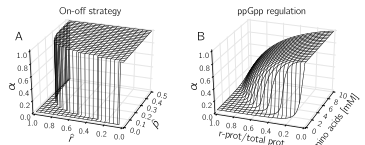
\includegraphics[scale=1]{./Fig/Fig8}
\caption{
\textbf{ppGpp regulation implements an on-off control strategy of resource allocation.}
\textit{A:}~Response surface of the on-off control strategy, defined by $\alpha = h(\hat{p},\hat{r})$ in Eq.~\ref{eq:stratswitch}.
\textit{B:}~Response surface of the ppGpp control strategy, as defined by Eq.~\ref{eq:ppGpp_empirical} and the simplified kinetic model defining ppGpp in terms of the total amino acid concentration and the ribosomal protein fraction (\ref{S4_Text}).
The shape of the response surface of the ppGpp control strategy is seen to be in very good agreement with the on-off strategy leading to near-optimal performance of the self-replicator during a nutrient upshift.
}
\label{fig:ppGppsurface}
\end{figure}

\section{Discussion}
\label{sec:discussion}

Quantitative growth laws are empirical regularities pointing at fundamental properties of microbial life~\cite{scott_bacterial_2011}.
Recent work has led to the precise theoretical formulation of growth laws and has shown that they can be derived from basic assumptions on the molecular processes responsible for the assimilation of nutrients and their conversion to biomass~\cite{bosdriesz_how_2015,maitra_bacterial_2014,molenaar_shifts_2009,scott_emergence_2014,weisse_mechanistic_2015}.
The growth laws are uniquely defined under the hypothesis that microorganisms allocate resources in such a way as to maximize their growth rate.
Several of the above-mentioned studies have analyzed feedback control strategies on the molecular level enabling cells to achieve optimal resource allocation in a robust manner.
The control strategies exploit information on the physiological state of the cell to adjust the (relative) rate of synthesis of different classes of proteins (ribsomes, metabolic enzymes, $\ldots$).
Whereas the growth laws describe microbial growth at steady state, most microorganisms live in complex, continuously changing environments.
Despite some precursory work~\cite{pavlov_optimal_2013,vandenberg_optimal_1998}, questions about the dynamics of microbial growth remain largely unanswered:
Which resource allocation schemes are optimal in changing environments? Which dynamical control strategies lead to (near-)optimal resource allocation? How do these strategies compare with those actually implemented by microorganisms? 

We have addressed the above questions by means of a self-replicator model of microbial growth, which, like other coarse-grained models of bacterial growth~\cite{maitra_bacterial_2014,molenaar_shifts_2009,scott_emergence_2014}, is capable of reproducing the growth laws at steady state (Fig.~\ref{fig:model_validation}).
A first major contribution of our work is to show that, in the case of a dynamical upshift scenario, optimal production of biomass requires a bang-bang-singular resource allocation scheme (Fig.~\ref{fig:optimalcontrol}).
That is, the optimal self-replicator should iteratively allocate all of its resources to the gene expression machinery (bang control input) and the metabolic machinery (another bang control input), until the steady state enabling maximal growth in the post-upshift environment is reached, corresponding to a trade-off in the allocation of resources to the two processes (singular control input).

Bang-bang phenomena are widespread in a variety of life processes.
Applications of optimal control theory to reproductive strategies in insects~\cite{macevicz_modeling_1976}, the development of intestinal crypts~\cite{itzkovitz_optimality_2012}, and the activation of metabolic pathways~\cite{bartl_modelling_2010,oyarzun_sequential_2009} have led to bang-bang or bang-bang-singular strategies.
In optimal control problems, such a solution arises with systems where the differential equations are linear in the control variable (in our case, $\alpha (\cdot)$).
Examples of applications that are close to the problem considered here are the control of gene expression for adaptation to environmental changes~\cite{pavlov_optimal_2013, madar_promoter_2013}, and the allocation of resources between nutrient uptake and growth in microorganisms~\cite{vandenberg_optimal_1998, kiselev_resource_2009}.
Whereas the former applications focus on minimization of response times, the latter also optimize biomass during a growth transition, using a different model, not derived from first principles as in this study.
However, the optimal solution of the corresponding optimal control problem is also bang-bang-singular, thus showing that our conclusions are robust to model variations.

Our second major contribution is the assessment of how different feedback control strategies perform with respect to each other and to the gold standard determined from optimal control theory.
We show that the precursor-only and nutrient-only strategies, both of which drive the self-replicator to the steady state with maximal growth rate in a static environment, perform quite differently in a dynamical upshift scenario (Fig.~\ref{fig:comparison_nutrients_precursor}).
While the precursor-only strategy is better than the nutrient-only strategy in a dynamical environment, it is in turn outperformed by a so-called on-off strategy, which achieves a near-perfect growth transition by exploiting information on the imbalance between the precursor concentration and the abundance of the gene expression machinery (Fig.~\ref{fig:onoffresults}).
The superior performance of the on-off strategy can be intuitively explained by the fact that during a growth transition the two variables are not fully correlated, which means that sensing both instead of either one provides additional information in a dynamical context.

Interestingly, the on-off strategy is based on a feedback control law that very much resembles the response function for ppGpp-mediated regulation of the synthesis of ribosomal RNAs in \textit{E. coli}~\cite{bosdriesz_how_2015}.
The role of ppGpp in controlling microbial growth has been amply documented~\cite{dalebroux_ppgpp_2012,potrykus_pppgpp_2008,hauryliuk_recent_2015}.
For example, Potrykus \textit{et al.} observed that in cells without ppGpp (ppGpp$^0$ mutants) the RNA/protein mass ratio, a proxy for our resource allocation variable $\alpha$, does not change with the growth rate, which has led these authors to conclude that ppGpp is the major source of growth-rate control in \textit{E. coli}~\cite{potrykus_ppgpp_2011}.
The central importance of ppGpp in the reallocation of gene expression resources in \textit{E. coli} following changes in nutrient availability has also been mapped with higher resolution, using genome-wide transcriptome studies~\cite{traxler_guanosine_2006,traxler_global_2008}.
In nearly all bacterial species examined so far, ppGpp is known to accumulate in response to an increase in the level of uncharged tRNA~\cite{gaca_many_2015}, although the molecular details of ppGpp metabolism and the range of other functions of the alarmone may greatly vary across species~\cite{gaca_many_2015,hauryliuk_recent_2015,liu_diversity_2015}.
While it has thus been well-established that regulation by ppGpp is an evolutionary conserved mechanism of growth control in the bacterial cell, our analysis provides a new perspective by suggesting that ppGpp enables optimal reallocation of resources after a growth transition, dynamically maximizing the accumulation of biomass.

The model on which the above results are based is built from first principles by distinguishing two fundamental cellular processes: metabolism (converting nutrients to precursors) and gene expression (converting precursors to the proteins that make up biomass) (Fig.~\ref{fig:self_replicator}). 
Despite its simplicity, our self-replicator model is capable of reproducing the empirical growth laws and of making testable predictions on the time-course profile of the resource allocation variable $\alpha$ and on the concentrations $p$ and $r$ of components of the gene expression machinery and metabolic machinery, respectively (see Fig.~\ref{fig:ppGppsurface} and below). 
The model can be easily extended with more details on protein synthesis, central carbon and energy metabolism, stress systems, or cell membranes, but this would make the mathematical analysis of the model dynamics and the optimal control problem more complicated. 
Notice, however, that the direct numerical approach for solving the optimal control problem remains applicable, even for more fine-grained models (Fig.~\ref{fig:optimalcontrol}, see also~\cite{waldherr_dynamic_2015}).

The comparison of different control strategies during a classical growth transition should be interpreted carefully, in a qualitative rather than quantitative manner. 
Whereas the differences in performance based on the biomass ratio $\texttt{Vol} / \texttt{Vol}_{opt}$ of the control strategies are robust, the absolute numbers for the biomass ratio will depend on details of the growth experiment chosen and the exact parameter values. 
Another implicit assumption in the analysis of the control strategies is that the costs of their molecular implementation can be neglected.
This is not true in general, since every control strategy requires resources to be diverted towards the synthesis of sensory systems and regulatory proteins, with possibly detrimental effects on growth.
In other words, a control strategy entails a trade-off between the growth burden of regulation and the growth benefit of the improved capability to adapt to changes in the environment~\cite{kalisky_costbenefit_2007,poelwijk_tradeoffs_2011}. 
The analysis of control strategies could be refined by adding a reaction to the self-replicator that models the loss of resources incurred by regulatory strategies.
While in general the growth burden of a control strategy requiring information on several aspects of cellular physiology is expected to be higher, notice that a single regulatory system may be capable of sensing more than one variable.
For example, we show that ppGpp levels in the cell carry information on both the metabolic and the gene expression state (Fig.~\ref{fig:ppGppsurface}), thus integrating several signals in a cost-efficient manner. 

The model predictions for the dynamical adaptation of resource allocation after a nutrient upshift suggest several interesting experimental tests.
In particular, the switching profile of the resource allocation variable $\alpha$ is a promising candidate for experimental validation. 
The most straightforward option would be direct measurement of the synthesis rate of ribosomal proteins, using a translational fusion of a fluorescent reporter with a ribosomal protein~\cite{bakshi_superresolution_2012,english_singlemolecule_2011}.
However, a more indirect approach based on the quantification of ppGpp concentrations in the cell or the activity of the ribosomal RNA (rRNA) promoters would also be a possibility.
Interestingly, some data are already available in the literature.
For instance, Gausing has reviewed data on the synthesis of ribosomal proteins after a nutrient upshift, showing that the synthesis rate goes through "a series of rapid changes" resembling oscillations~\cite{gausing_regulation_1980}.
Later work attributed this pattern to regulation on the transcriptional level~\cite{zengel_transcription_1986}.
Friesen \textit{et al.} observed oscillatory patterns in ppGpp concentrations after a nutrient upshift, with an initial response resembling bang control for an upshift to a particularly rich medium~\cite{friesen_synthesis_1975}.
Murray \textit{et al.} also present data on the ppGpp concentration after a nutrient upshift~\cite{murray_control_2003}, but with a lower temporal resolution and no clear oscillatory pattern.
All of the above measurements were carried out on the population level, which means that switching patterns may be obscured by desynchronisation of the individual cells.
More sophisticated experimental set-ups are necessary for the decisive validation of the model predictions, allowing gene expression in single cells to be followed over time in tightly regulated growth conditions~\cite{young_measuring_2011,duncombe_microfluidics_2015}.
In addition, the model could be validated on other dynamical scenarios, for example nutrient downshifts~\cite{molin_control_1977,murray_control_2003}.

Apart from its interest for fundamental science, resource allocation is also a critical question in biotechnology, where there exists an inherent trade-off between the maximization of yield and productivity\cite{venayak_engineering_2015}.
High yield means that most of the substrate is converted to a metabolite, peptide or recombinant protein of interest, but this leads to low productivity if the remaining nutrient influx is insufficient to sustain population growth.
Engineered control of resource allocation may help in establishing the right trade-off, the most profitable balance between yield and productivity, in a biotechnological process.
Such a trade-off could be attained either in steady-state conditions (the incoming nutrient flux is optimally distributed over growth and production) or in dynamical conditions (alternating utilization of the incoming nutrient flux for growth or production)~\cite{dahl_engineering_2013,xu_improving_2014,izard_synthetic_2015}.
When extended with heterologous metabolic pathways, the self-replicator models used in this study would provide an adequate \textit{in-silico} test bed for the rapid screening and comparison of alternative control strategies in bioprocess engineering.
 
%%%%%%%%%%%%%%%%%%%%%%%%%%%%%%%%

\section{Methods}

\subsection{Steady-state analysis of model}
\label{sec:methods_model_analysis}

The nondimensional version of the model, given by Eqs~\ref{eq:pdefnondim}-\ref{eq:rdefnondim}, was used for a steady-state analysis of the self-replicator.
Eqs~\ref{eq:pdefnondim}-\ref{eq:rdefnondim} were derived from the original model of Eqs~\ref{eq:pdef}-\ref{eq:rdef} by means of the following rescalings:
\begin{equation*}
\hat{p}  = \beta \, p,\;\;\;
\hat{r}  = \beta \, r,\;\;\;
\hat{t}  = k_R \, t,\;\;\;
E_M = e_M/k_R,\;\;\;
K = \beta K_R.
\end{equation*}

As shown in \ref{S1_Text}, for a constant environment $E_M$ and constant resource allocation $\alpha$, the system has two steady states: a trivial unstable steady state $(\hat{p}^*, \hat{r}^*) = (0,1)$, allowing no growth in the absence of precursors, and a steady state with a positive growth rate given by
\begin{equation}
\label{eq:meth_steadystate}
(\hat{p}^*, \hat{r}^*) = \left( \frac{(1-\alpha)\, E_M - \alpha + \sqrt{[(1-\alpha)\, E_M - \alpha]^2 + 4\alpha\, (1-\alpha)\, E_M\, K}}{2\alpha}, \alpha \right).
\end{equation}
The two eigenvalues of the Jacobian matrix evaluated at $(\hat{p}^*, \hat{r}^*)$ are negative (\ref{S1_Text}), so that this steady state is stable.

The growth rate at steady state, as a function of $\hat{p}^*$ and $\hat{r}^*$, is given by Eq.~\ref{eq:munondim}, which we repeat here for clarity:
\begin{equation*}
\hat{\mu}^* = \frac{\hat{p}^*}{K + \hat{p}^*} \, \hat{r}^* .
\end{equation*}
Evaluating $d\hat{p}/dt=0$ at $(\hat{p}^*, \hat{r}^*)$ allows $\hat{r}^*$, and therefore $\hat{\mu}^*$, to be written as a function of $\hat{p}^*$ (\ref{S1_Text}).
Accordingly, we can compute $\partial\hat{\mu}^*/\partial\hat{p}^*$ and, when setting this partial derivative to 0, determine the maximum growth rate at steady state $\mu_{opt}^*$ and the optimal resource allocation $\alpha_{opt}^*$ bringing about this maximal growth rate.
As shown in \ref{S1_Text}, $\mu_{opt}^*$ and $\alpha_{opt}^*$ can be written as explicit functions of either the environment $E_M$:
\begin{equation}
\label{eq:alpha_mu_optimal}
\alpha_{opt}^* = \frac{E_M + \sqrt{K\, E_M}}{E_M + 2\sqrt{K\, E_M} + 1}
, \;\;\;\;\;\;\;\;\;\;\;\;\;\; 
\hat{\mu}^*_{opt} = \frac{E_M}{E_M + 2\sqrt{K\, E_M} + 1},
\end{equation}
or the precursor abundance $\hat{p}_{opt}^*$:
\begin{equation}
\label{eq:alpha_mu_optimal_p}
\alpha_{opt}^* = \frac{\hat{p}^{*}_{opt}}{\hat{p}^{*}_{opt} + \frac{K}{K+\hat{p}^{*}_{opt}}(1+\hat{p}^{*}_{opt})}
, \;\;\;\;\;\;\;\;\;\;\;\;\;\; 
\hat{\mu}^*_{opt} = \frac{\hat{p}^{* 2}_{opt}}{\hat{p}^{* 2}_{opt} + 2K\hat{p}^*_{opt} + K}.
\end{equation}
The above equations were used for the derivation of the control strategies (see below).


\subsection{Model fitting}
\label{sec:methods_model_fitting}

As can be seen by comparing Figs~\ref{fig:model_validation}\textit{A} and~\ref{fig:model_validation}\textit{B}, growth-rate maximization in the self-replicator model leads to a good qualitative correspondence with the growth laws.
In order to determine if a good quantitative fit of the model with the data from Scott~\textit{et al.} \cite{scott_interdependence_2010} can be obtained, for reasonable parameter values, we estimated $e_M$ and $k_R$ in Eqs~\ref{eq:pdef}-\ref{eq:rdef} from the measured RNA/protein mass ratios.
At steady state, the RNA/protein mass ratio can be interpreted as proportional to $\hat{r}^*$ (and thus $\alpha_{opt}^*$), with an unknown (dimensionless) proportionality constant $\gamma$ (see~\cite{scott_interdependence_2010} for details on the use of the RNA/protein mass ratio as a proxy for the ribosomal protein mass fraction):
\begin{equation}
\hat{r}^* = \alpha_{opt}^* = \gamma \, \frac{\text{RNA mass}}{\text{protein mass}}.
\label{eq:gamma}
\end{equation}
Reformulating Eq.~\ref{eq:alpha_mu_optimal} in terms of the original parameters $e_M$ and $k_R$, which have physical dimensions facilitating the biological interpretation of their values, we obtain a straighforward relation between $e_M$, $k_R$, $K$, $\alpha_{opt}^*$ and $\mu_{opt}^*$:
\begin{equation}
\label{eq:alpha_mu_optimal_dim}
\alpha_{opt}^* = \frac{e_M + \sqrt{K\, e_M\, k_R}}{e_M + 2\sqrt{K\, e_M\, k_R} + k_R}
, \;\;\;\;\;\;\;\;\;\;\;\;\;\; 
\mu^*_{opt} = \frac{e_M \, k_R}{e_M + 2\sqrt{K\, e_M\, k_R} + k_R}.
\end{equation}

Eqs~\ref{eq:gamma}-\ref{eq:alpha_mu_optimal_dim} were used to estimate values of $k_R$ and $\gamma$, as well as $e_M$ for each of the six growth conditions, from the measurements of the growth rate and the RNA/protein mass ratio. 
The value $K$ was not estimated from the experimental data, but set to a value inferred from the literature (\ref{S1_Text}).
The optimization process was carried out by means of the differential evolution algorithm of Storn and Price~\cite{storn_differential_1997}.
The results are shown in Fig.~\ref{fig:model_validation}\textit{B}, while the estimated parameter values are summarized in \ref{S1_Table}.
The parameter values are in very good agreement with order-of-magnitude values determined from the literature (\ref{S2_Text} and \ref{S1_Table}). 

\subsection{Solution of optimal control problem}

The optimal control problem of Eq.~\ref{eq:J} consists in identifying the function $\alpha_{opt}(t)$ that maximizes the integral of the growth rate $\hat{\mu}$ over an interval $[0, \tau]$.
In order to solve this problem, we first redefined it over an infinite horizon (\textit{i.e.}, $\tau \rightarrow \infty $) in order to avoid boundary effects occurring over finite time intervals, in particular the depletion of precursors just before reaching $\tau$.
With $\mathcal{U}=\{\alpha:\mathbb{R}^+ \rightarrow [0,1] \}$ the set of admissible controls, the full optimization problem for the nondimensionalized system is given by
\begin{equation}\label{eq:meth_prob}
\max_{\alpha \in \mathcal{U}} J(\alpha)\equiv \int_0^{\infty} \hat{r}(\hat{t}) \, \dfrac{\hat{p}(\hat{t})}{K+\hat{p}(\hat{t})}\, d\hat{t}.
\end{equation}
Since $J(\alpha)$ diverges, we actually consider overtaking optimality:
A solution is overtaking optimal if its performance index catches up with the performance index of any other solution (\cite{carlson_infinite_1991}, see \ref{S3_Text} for details).

Necessary conditions on optimal trajectories can be obtained by the Infinite Horizon Maximum Principle \cite{carlson_infinite_1991}, an extension of the well-known Pontryagin Maximum Principle.
Analysis of the Hamiltonian of the system of Eqs~\ref{eq:pdefnondim}-\ref{eq:rdefnondim} and the associated adjoint system shows that the optimal trajectory is a concatenation of bang arcs ($\alpha(\cdot)=0$ or $\alpha(\cdot)=1$) and possibly a singular arc corresponding to the optimal steady state $(\hat{p}(t),\hat{r}(t))=(\hat{p}_{opt}^*,\hat{r}_{opt}^*)$, that is, the steady state leading to the optimal growth rate $\hat{\mu}_{opt}^*$ in the new environment after the upshift (\ref{S3_Text}).
Moreover, from the Kelley condition~\cite{borisov_fullers_2000}, we can show that if the optimal trajectory has a singular arc, then it must enter this singular arc \textit{via} a chattering arc, \textit{i.e.}, with an infinite number of switches of $\alpha (\cdot)$ between 0 and 1 (\ref{S3_Text}).
The chattering arc is characterized by a switching curve $\hat{r}=\varphi(\hat{p})$ in the $(\hat{p},\hat{r})$-plane, which passes through $(\hat{p}_{opt}^*,\hat{r}_{opt}^*)$.
The switching curve divides the phase plane into two regions, such that $\alpha(t)$ switches to 0 when the system is in the region above $\varphi$ and to 1 when the system is below $\varphi$ (\ref{S3_Text} and Fig.~\ref{fig:optimalcontrol}).

The above results have led to the conjectured optimal solution of Eq.~\ref{eq:optcontrol}.
In parallel, we numerically solved the problem of Eq.~\ref{eq:meth_prob} by a direct method using the \texttt{bocop} software~\cite{bonnans_bocop_2012}.
A time discretization allows the optimal control problem to be transformed into a nonlinear optimization problem,
solved here by interior point techniques.
A discretization by a Lobatto IIIC formula (6th order) was used with 4000 time steps, and the relative tolerance for the NLP solver was set to $10^{-14}$.
The optimal trajectories thus obtained are composed of a chattering arc followed by a steady state corresponding to the singular arc (Fig.~\ref{fig:optimalcontrol}).
The switching curve $\varphi(\hat{p})$ was computed from numerical simulations with different initial conditions. 

\subsection{Specification and analysis of control strategies}

As described in the \textit{Results} section, we are interested in control strategies satisfying the following conditions:
\begin{description}
\item[(C1)] The control laws are static functions of the system variables (as opposed to, for instance, functions that depend on derivatives or integrals of the variables).
\item[(C2)] For any given constant environment $E_M$, they drive the self-replicator system towards a unique stable steady state that is not trivial, \textit{i.e.}, with nonzero growth rate.
\item[(C3)] This steady state corresponds to the optimal steady state $(\hat{p}_{opt}^*, \hat{r}_{opt}^*)$, allowing growth at the maximal rate $\mu^*_{opt}$.
\end{description}
It can be directly verified from the functions $f$, $g$, and $h$ defining the nutrient-only, precursor-only, and on-off control strategies (Eqs~\ref{eq:f}, \ref{eq:precursorstrategy}, and \ref{eq:stratswitch}) that they are indeed static functions of the system variables (or the system input, in the case of the nutrient-only strategy). 
Here we show that the other two conditions are also satisfied for all three strategies.

Following Eq.~\ref{eq:f}, the nutrient-only strategy is defined by $\alpha = f(E_M)$, so that $\alpha$ is constant after the upshift.
As shown above and in \ref{S1_Text}, this means that the system controlled by the nutrient-only strategy has a single nontrivial stable steady state (Condition~C2). 
In addition, in this case the optimal steady state is attained for $\alpha^*_{opt}$ defined as in Eq.~\ref{eq:alpha_mu_optimal}, and the following function $f$ therefore guarantees Condition~C3:
\begin{equation}
\label{eq:meth_f}
f(E_M) = \frac{E_M + \sqrt{K E_M}}{E_M + 2\sqrt{K\, E_M} + 1}.
\end{equation}
In \ref{S1_Text}, it is shown that Eq.~\ref{eq:meth_f} is the only definition of $f$ satisfying all conditions.
\ref{S1_Fig} shows a plot of $f(E_M)$ together with a biologically plausible Michaelis-Menten approximation (Eq.~\ref{eq:MMApprox}).

The full specification of the precursor-only strategy demands an expression for the function $g$ in Eq.~\ref{eq:precursorstrategy}.
Recall that Eq.~\ref{eq:alpha_mu_optimal_p} defines $\alpha_{opt}^*$ in terms of the precursor concentration $\hat{p}_{opt}^*$, which leads us to propose the following function $g$:
\begin{equation}
\label{eq:meth_g}
g(\hat{p}) = \frac{\hat{p}}{\hat{p} + \frac{K}{K + \hat{p}}(1+\hat{p})}.
\end{equation}
As shown in \ref{S1_Text} by computing the Jacobian, the system given by Eqs~\ref{eq:pdefnondim}-\ref{eq:rdefnondim} and \ref{eq:meth_g} has a single nontrivial stable steady state for any environment $E_M$ (Condition~C2).
Moreover, Eq.~\ref{eq:meth_g} guarantees this steady state to be optimal (Condition~C3).
This can be seen by noting that at steady state, $d\hat{r}/dt=0$ implies $\hat{r}^*=g(\hat{p}^*)$ (Eq.~\ref{eq:rdefnondim}).
In order for the self-replicator to attain a maximal growth rate at steady rate, Eq.~\ref{eq:alpha_mu_optimal_p} needs to be satified, which is the case for the above choice of the function $g$.
Like for $f$, Eq.~\ref{eq:meth_g} is the only choice for $g$ satisfying C1-C3.
\ref{S1_Fig} shows a plot of $g(\hat{p})$ together with a biologically plausible Hill approximation (Eq.~\ref{eq:HillApprox}).

The on-off control strategy is defined in Eq.~\ref{eq:stratswitch} and repeated below:
\begin{equation}
h(\hat{p}, \hat{r}) = 
\begin{cases}
0, \ \textrm{if} \ \hat{r} > g(\hat{p}),\\
1, \ \textrm{if} \ \hat{r} < g(\hat{p}), \\
\alpha_{opt}^*, \ \textrm{if} \ (\hat{p},\hat{r})=(\hat{p}_{opt}^*,\hat{r}_{opt}^*).
\end{cases}
\end{equation}
This strategy drives the system to a single steady state, because the $\hat{p}$-nullcline crosses the function $g(\hat{p})$ only once, as shown graphically in Fig.~\ref{fig:onoffresults}\textit{A}.
In \ref{S1_Text} we argue that this steady state is stable, by taking into account so-called sliding modes on the switching curve~\cite{filippov_differential_1988} (Condition~C2).
Moreover, the steady state coincides with the optimal steady state $(\hat{p}_{opt}^*,\hat{r}_{opt}^*)$ by construction, so that Condition~C3 is satisfied as well.
Fig~\ref{fig:ppGppsurface}\textit{A} shows a plot of $h(\hat{p}, \hat{r})$.

Note that since $h(\cdot)$ is discontinuous, numerical instabilities occur during simulations.
We therefore used the following continuous approximation of this function:
\begin{equation}
\frac{g(\hat{p})^{100}}{g(\hat{p})^{100} + \hat{r}^{100}}, \ \textrm{if} \ \hat{r} \neq g(\hat{p}).
\end{equation}
The approximation causes $\alpha$ to take intermediate values (instead of 0 or 1) just before reaching the optimal steady state in Fig~\ref{fig:onoffresults}\textit{C}.
For numerical simulations of the ODE system, we used the CVODE solver~\cite{cohen_cvode_1996} from SUNDIALS 2.6.2~\cite{hindmarsh_sundials_2005}.

\clearpage

\section{Supporting information for Chapter~2}

\subsection{S1 Text -- Model derivation and analysis}
\manuallabel{S1_Text}{S1~Text}

\subsubsection{Model formulation}

The time evolution of the total mass of each component of the self-replicator can be written as follows:
\begin{eqnarray}
\frac{dP}{dt} &=& V_M(t) - V_R(t) \nonumber , \\
\frac{dM}{dt} &=& (1-\alpha(t))\, V_R(t) \label{eq:ext_system},\\
\frac{dR}{dt} &=& \alpha(t) \, V_R(t)  \nonumber ,
\end{eqnarray}
where $P$, $M$, $R$ [g] denote the total mass of precursors, metabolic machinery and gene expression machinery, respectively.
$V_M$ [g h$^{-1}$] is the rate of production of precursors by metabolism and $V_R$ [g h$^{-1}$] the rate of utilisation of precursors for gene expression.

Dividing the mass variables by the total time-varying volume $\texttt{Vol}(t)$ of the system, we obtain the concentration variables $p = P/\texttt{Vol}$, $m = M/\texttt{Vol}$, $r = R/\texttt{Vol}$ [g L$^{-1}$].
The dynamics of the concentration variables then follows with Eq.~\ref{eq:ext_system}:
\begin{eqnarray}
\frac{dp}{dt} &=& \frac{V_M(t)}{\texttt{Vol}} - \frac{V_R(t)}{\texttt{Vol}} - \frac{1}{\texttt{Vol}}\frac{d\texttt{Vol}}{dt}\, p, \nonumber \\
\frac{dm}{dt} &=& (1-\alpha(t)) \frac{V_R(t)}{\texttt{Vol}} - \frac{1}{\texttt{Vol}}\frac{d\texttt{Vol}}{dt} \, m  \label{eq:deriv_int_system},\\ 
\frac{dr}{dt} &=& \alpha(t) \, \frac{V_R(t)}{\texttt{Vol}}  - \frac{1}{\texttt{Vol}}\frac{d\texttt{Vol}}{dt} \, r. \nonumber
\end{eqnarray}

At this point, we define $v_M = V_M/\texttt{Vol}$ and $v_R = V_R/\texttt{Vol}$ [g L$^{-1}$ h$^{-1}$] as the mass fluxes per unit volume.
Moreover, with the definition of the volume in terms of the total protein mass in Eq.~\ref{eq:voldef} of the main text, that is, $\texttt{Vol} = \beta\, (M + R)$, we find that
\begin{equation}
\label{eq:supp_deriv_growthrate}
\frac{1}{\texttt{Vol}} \frac{d\texttt{Vol}}{dt} = \frac{\beta}{\texttt{Vol}} \frac{d(M+R)}{dt} = \beta\, \frac{V_R(t)}{\texttt{Vol}} = \beta \, v_R(t).
\end{equation}
This leads to the system
\begin{eqnarray}
\frac{dp}{dt} &=& v_M(t) - v_R(t) \, (1+\beta\, p), \label{eq:supp_pdef}\\
\frac{dr}{dt} &=& v_R(t)  \, (\alpha(t) - \beta\, r) \label{eq:supp_rdef},
\end{eqnarray}
where the equation for $m(t)$ is omitted since by construction $r(t) + m(t) = 1/\beta$ and $dr/dt + dm/dt = 0$.

As stated in the main text, we use Michaelis-Menten kinetics to express $v_M$ and $v_R$ in terms of the system variables:
\begin{eqnarray}
v_M(t) &=& m(t) \, k_M \, \frac{s(t)}{K_M +s(t)} = \left(\frac{1}{\beta} - r(t)\right)\, e_M(t) \nonumber, \\
v_R(t) &=& r(t) \, k_R \, \frac{p(t)}{K_R +p(t)}, \nonumber 
\end{eqnarray}
with rate constants $k_M$, $k_R$ [h$^{-1}$] and half-saturation constants $K_M$, $K_R$ [g L$^{-1}$].
$s(t)$ is an exogenous variable representing the nutrient concentration in the external medium.
We simplify $v_M(t)$ by defining the environmental input $e_M(t) = k_M \, s(t) / (K_M + s(t))$.
Throughout the paper, as explained in the main text, we assume the environment is constant, \textit{i.e.}, $e_M(t)=e_M$.

Finally, the growth rate $\mu$ [h$^{-1}$] is defined as the relative increase of the volume of the self-replicator.
From Eq.~\ref{eq:supp_deriv_growthrate}, it follows that:
\begin{equation}
\label{eq:supp_growthrate}
\mu (t) = \frac{1}{\texttt{Vol}} \frac{d\texttt{Vol}}{dt} = \beta\, v_R(t).
\end{equation}

\subsubsection{Nondimensionalization of the system}

For the sake of simplifying the proofs and derivations below, we define the following nondimensional variables:
\begin{equation*}
\hat{p}  = \beta \, p,\;\;\;
\hat{r}  = \beta \, r,\;\;\;
\hat{t}  = k_R \, t.
\end{equation*}
When injecting these into Eq.~\ref{eq:supp_pdef}, we obtain
\[
\frac{k_R}{\beta} \, \frac{d\hat{p}}{d\hat{t}} = \left( \frac{1}{\beta} - \frac{\hat{r}}{\beta} \right) \, e_M - \frac{\hat{r}}{\beta} \, k_R \, \frac{\hat{p}}{\beta K_R + \hat{p}} \, (1 + \hat{p}),
\]
which simplifies to
\[
\frac{d\hat{p}}{d\hat{t}} = ( 1 - \hat{r} ) \, \frac{e_M}{k_R} - \hat{r} \, \frac{\hat{p}}{\beta K_R + \hat{p}} \, (1 + \hat{p}).
\]
In a similar manner, we derive the time evolution of the nondimensional $\hat{r}$, and thus obtain the system
\begin{equation}
\label{eq:supp_adim}
\begin{aligned}
\frac{d\hat{p}}{d\hat{t}} &= (1-\hat{r})\, E_M - (1 + \hat{p}) \, \frac{\hat{p}}{K + \hat{p}}\, \hat{r},\\
\frac{d\hat{r}}{d\hat{t}} &= (\alpha - \hat{r}) \, \frac{\hat{p}}{K + \hat{p}}\, \hat{r},
\end{aligned}
\end{equation}
with the lumped parameters $E_M = e_M / k_R$ and $K = \beta \, K_R$.
The corresponding nondimensionalized growth rate is given by
\begin{equation}
\label{eq:supp_growthrate_adim}
\hat{\mu} = \frac{\mu}{k_R} = \frac{\hat{p}}{K+\hat{p}} \, \hat{r}.
\end{equation}

\subsubsection{Steady-state growth of the self-replicator}
\label{si::growthrate}

If we suppose $E_M > 0$, $K > 0$ and $\alpha \in ]0, 1[$, there is a trivial unstable steady state at $(0, 1)$.
A second steady-state exists for the point in which $\hat{r}^* = \alpha$ and $\hat{p}^*$ is a root of the following polynomial:
\[
\alpha \, \hat{p}^2 + \left(\alpha - (1-\alpha) \, E_M \right) \hat{p} - (1-\alpha)\, E_M\, K.
\]
If we keep the only admissible root for this polynomial (\textit{i.e.}, for which $\hat{p} \geq 0$), the second steady state is given by
\begin{equation}
\label{eq:supp_steadystate}
(\hat{p}^*, \hat{r}^*) = \left( \frac{(1-\alpha)\, E_M - \alpha + \sqrt{[(1-\alpha)\, E_M - \alpha]^2 + 4\alpha\, (1-\alpha)\, E_M\, K}}{2\alpha}, \alpha \right).
\end{equation}
We can determine the stability of this steady state by looking at the Jacobian matrix $J$ of the ODE system:
\begin{equation}
\label{eq:supp_jacop}
J = \left(\begin{matrix}
- \frac{\hat{r}}{K + \hat{p}} \left[ \hat{p} + (1+\hat{p})\, \frac{K}{K+\hat{p}}\right] & - E_M - (1+\hat{p})\frac{\hat{p}}{K+\hat{p}}\\
(\alpha - \hat{r})\, \hat{r} \, \frac{K}{(K+\hat{p})^2} & (\alpha - 2\hat{r})\, \frac{\hat{p}}{K+\hat{p}}
\end{matrix}\right) .
\end{equation}
Evaluated at the point $(\hat{p}^*, \hat{r}^*)$, the Jacobian matrix becomes
\[
J_{(\hat{p}^*, \hat{r}^*)} = \left(\begin{matrix}
- \frac{\alpha}{K + \hat{p}^*} \left[ \hat{p}^* + (1+\hat{p}^*)\frac{K}{K+\hat{p}^*}\right] & - E_M - (1+\hat{p}^*)\frac{\hat{p}^*}{K+\hat{p}^*}\\
0 & -\alpha\frac{\hat{p}^*}{K+\hat{p}^*}
\end{matrix}\right).
\]
Since $\hat{p}^*$, $\alpha$, $E_M$, $K$ $>0$, the two eigenvalues are negative and therefore the steady state $(\hat{p}^*, \hat{r}^*)$ is stable (see also the streamlines in Figure~\ref{fig:model_analysis}\textit{A} in the main text).
It means that for fixed environmental conditions $E_M$ and resource allocation $\alpha$, the self-replicator converges towards a steady state in which the concentration variables are constant.

One can now easily derive the steady-state growth rate, denoted $\hat{\mu}^*$.
By substituting Eq.~\ref{eq:supp_growthrate_adim} into the first ODE of the system of Eq.~\ref{eq:supp_adim}, we find at steady state:
\[
\left(\frac{d\hat{p}}{d\hat{t}}\right)_{(\hat{p}^*, \hat{r}^*)} = 0 = (1-\alpha)\, E_M - (1+\hat{p}^*)\, \hat{\mu}^*,
\]
which by means of Eq.~\ref{eq:supp_steadystate} gives the following relation:
\begin{equation}
\label{eq:supp_growthrate_p}
\begin{split}
\hat{\mu}^* &= \frac{(1-\alpha)\, E_M}{1+\hat{p}^*}\\
 &= \frac{2\alpha(1-\alpha)\, E_M}{(1-\alpha)\, E_M + \alpha + \sqrt{\left[(1-\alpha)\, E_M -\alpha\right]^2 + 4\alpha(1-\alpha)\, E_M\, K}}.
\end{split}
\end{equation}
Finally, we can transform this expression to obtain
\begin{equation}
\label{eq:supp_growthrate_final}
\hat{\mu}^* = \begin{cases}
\frac{(1-\alpha)\, E_M + \alpha - \sqrt{\left[(1-\alpha)\, E_M - \alpha\right]^2 + 4(1-\alpha)\, \alpha\, E_M\, K}}{2(1-K)} &\text{ for }K\neq 1,\\
\frac{\alpha\, (1-\alpha)\, E_M}{\alpha + (1-\alpha)\, E_M} &\text{ for }K = 1.
\end{cases}
\end{equation}
This function of $\alpha$ is plotted in Figure~\ref{fig:model_analysis}\textit{B} in the main text.

\subsubsection{Maximization of growth rate at steady state}
\label{si::optimal}

We are interested in the steady state at which growth occurs at the maximum rate.
The growth rate at steady state $\hat{\mu}^*$ is given by
\begin{equation}
\label{eq:supp_growthrate_steadystate}
\hat{\mu}^* = \frac{\hat{p}^*}{K + \hat{p}^*} \, \hat{r}^* .
\end{equation}
From the first ODE of the system of Eq.~\ref{eq:supp_adim}, we have
\begin{equation}
\label{eq:supp_isop}
\hat{r}^* = \frac{E_M}{E_M + \frac{\hat{p}^*}{K + \hat{p}^*} (1+\hat{p}^*)} .
\end{equation}
Substituting Eq.~\ref{eq:supp_isop} into Eq.~\ref{eq:supp_growthrate_steadystate}, we obtain
\begin{equation}
\label{eq:supp_growthrate_steadystate_p}
\hat{\mu}^* = \frac{E_M \, \hat{p}^*}{\hat{p}^{* 2} + (E_M + 1)\, \hat{p}^* + E_M\, K} .
\end{equation}
The value of $\hat{p}^*$ maximizing $\hat{\mu}^*$ can be determined from
\begin{equation}
\label{eq:supp_growthrate_steadystate_deriv_p}
\frac{\partial\hat{\mu}^*}{\partial\hat{p}^*} = \frac{E_M \, (E_M\, K - \hat{p}^{*2})}{\left(\hat{p}^{* 2} + (E_M + 1)\, \hat{p}^* + E_M\, K\right)^2},
\end{equation}
by looking at the values of $\hat{p}^*$ for which this derivative equals 0.
It follows that $\hat{\mu}^*$ is maximal for
\begin{equation}
\label{eq:supp_p_optimal}
\hat{p}^* = \hat{p}^*_{opt} = \sqrt{K\, E_M}.
\end{equation}
By substituting $\hat{p}^*_{opt}$ and $\alpha_{opt}^*$ for $\hat{p}^*$ and $\hat{r}^*$, respectively, in Eq.~\ref{eq:supp_isop}, we obtain the resource allocation maximizing the growth rate
\begin{equation}
\label{eq:supp_alpha_optimal}
\alpha_{opt}^* = \frac{E_M + \sqrt{KE_M}}{E_M + 2\sqrt{KE_M} + 1}.
\end{equation}
Finally, injecting this result into Eq.~\ref{eq:supp_growthrate_steadystate} we obtain the optimal steady-state growth rate:
\begin{equation}
\label{eq:supp_growthrate_optimal}
\hat{\mu}^*_{opt} = \frac{E_M}{E_M + 2\sqrt{K\, E_M} + 1}.
\end{equation}
In addition, by using Eq. \ref{eq:supp_p_optimal}, we can write $\alpha_{opt}^*$ and $\hat{\mu}_{opt}^*$ as a function of $\hat{p}_{opt}^*$ only:
\begin{equation}
\label{eq:supp_alpha_mu_optimal_p}
\alpha_{opt}^* = \frac{\hat{p}^{*}_{opt}}{\hat{p}^{*}_{opt} + \frac{K}{K+\hat{p}^{*}_{opt}}(1+\hat{p}^{*}_{opt})}
, \;\;\;\;\;\;\;\;\;\;\;\;\;\; 
\hat{\mu}^*_{opt} = \frac{\hat{p}^{* 2}_{opt}}{\hat{p}^{* 2}_{opt} + 2K\hat{p}^*_{opt} + K}.
\end{equation}

\subsubsection{Analysis of the control strategies}
\label{si::control_strategies}

In this section, we derive the main results for the functions $f$, $g$, and $h$ defining the nutrient-only, precursor-only, and on-off control strategies.
For each of these, we prove that the Conditions C1, C2 and C3 from the \textit{Methods} section are satisfied, which we repeat here for clarity:
\begin{description}
\item[(C1)] The control laws are static functions of the system variables (as opposed to, for instance, functions that depend on derivatives or integrals of the variables).
\item[(C2)] For any given constant environment $E_M$, they drive the self-replicator system towards a unique stable steady state that is not trivial, \textit{i.e.}, with nonzero growth rate.
\item[(C3)] This steady state corresponds to the optimal steady state $(\hat{p}_{opt}^*, \hat{r}_{opt}^*)$, allowing growth at the maximal rate $\mu^*_{opt}$.
\end{description}

\paragraph{Nutrient-only strategy}

The nutrient-only strategy is defined by:
\begin{equation}
\label{eq:supp_f}
\alpha = f(E_M) = \frac{E_M + \sqrt{K E_M}}{E_M + 2\sqrt{K\, E_M} + 1}.
\end{equation}
It drives the system to the optimal steady state by measuring the environment $E_M$.
Note that Condition C1 is satisfied by definition.

By injecting Eq.~\ref{eq:supp_f} into Eq.~\ref{eq:supp_adim}, the ODE system under the control of $f$ becomes:
\begin{equation}
\label{eq:supp_adim_f}
\begin{aligned}
\frac{d\hat{p}}{d\hat{t}} &= (1-\hat{r})\, E_M - (1 + \hat{p}) \, \frac{\hat{p}}{K + \hat{p}}\, \hat{r},\\
\frac{d\hat{r}}{d\hat{t}} &= \left(f(E_M) - \hat{r} \right) \, \frac{\hat{p}}{K + \hat{p}}\, \hat{r}.
\end{aligned}
\end{equation}
Since $E_M$ is constant on the interval of interest (starting right after the upshift), we are in the case of Section~\ref{si::growthrate} (\textit{i.e.}, $\alpha$ constant).
In particular, the system has two steady states: a trivial unstable one at (0, 1) (with zero growth), and a stable one defined by Eq.~\ref{eq:supp_steadystate} (Condition C2).
Since $f(E_M) = \alpha_{opt}^*$, we conclude from the derivations in Section~\ref{si::optimal} that the stable steady state is optimal for every environment $E_M$ (Condition C3).

It is interesting to note that the expression in Eq.~\ref{eq:supp_f} is the only function $f(E_M)$ satisfying C1-C3.
We can prove this statement by contradiction.
Assume a control strategy $c(E_M)$ satisfying C1-C3, and different from $f(E_M)$, \textit{i.e.}, there exists $E_M={E_M}_1$ such that $c({E_M}_1) \neq f({E_M}_1)$.
In this environment, the system reaches a steady state $(\hat{p}_1^*, \hat{r}_1^*)$ with $\hat{r}_1^* = c({E_M}_1) \neq f({E_M}_1)$.
However, by Eq.~\ref{eq:supp_alpha_optimal} the optimal value for $\hat{r}^*$ in this environment is given by $f({E_M}_1)$.
So, the control law $c(E_M)$ does not drive the system to the optimal steady state in this environment, in contradiction with Condition~C3.

\paragraph{Precursor-only strategy}

The precursor-only strategy is defined by:
\begin{equation}
\label{eq:supp_g}
\alpha = g(\hat{p}) = \frac{\hat{p}}{\hat{p} + \frac{K}{K + \hat{p}}(1+\hat{p})}.
\end{equation}
Here as well, C1 is satisfied by construction.

The ODE system under the control of $g$ becomes
\begin{equation}
\label{eq:supp_adim_g}
\begin{aligned}
\frac{d\hat{p}}{d\hat{t}} &= (1-\hat{r})\, E_M - (1 + \hat{p}) \, \frac{\hat{p}}{K + \hat{p}}\, \hat{r},\\
\frac{d\hat{r}}{d\hat{t}} &= \left(g(\hat{p}) - \hat{r} \right) \, \frac{\hat{p}}{K + \hat{p}}\, \hat{r}.
\end{aligned}
\end{equation}
The nullcline for $\hat{p}$ remains unchanged and is defined by
\begin{equation}
\label{eq:supp_pnullcline_g}
\frac{d\hat{p}}{dt} = 0 \Leftrightarrow 
\hat{r} = \frac{E_M}{E_M + \frac{\hat{p}}{K+\hat{p}} (1+\hat{p})},
\end{equation}
while the nullcline for $\hat{r}$ is
\begin{equation}
\label{eq:supp_rnullcline_g}
\frac{d\hat{r}}{dt} = 0 \Leftrightarrow \begin{cases}
\hat{p} = 0,\\
\hat{r} = 0,\\
\hat{r} = \frac{\hat{p}}{\hat{p} + \frac{K}{K+\hat{p}} (1+\hat{p})}.
\end{cases}
\end{equation}
Hence, we also have a trivial unstable steady state at (0,1) (with zero growth).
The second steady state is obtained from Eqs~\ref{eq:supp_pnullcline_g}-\ref{eq:supp_rnullcline_g}:
\begin{equation*}
\frac{E_M}{E_M + \frac{\hat{p}^*}{K+\hat{p}^*} (1+\hat{p}^*)} = \frac{\hat{p}^*}{\hat{p}^* + \frac{K}{K+\hat{p}^*} (1+\hat{p}^*)},
\end{equation*}
which we rearrange into
\begin{equation*}
\hat{p}^* E_M + \frac{K}{K+\hat{p}^*} (1+\hat{p}^*) E_M = \hat{p}^* E_M + \frac{\hat{p}^*}{K+\hat{p}^*} (1+\hat{p}^*) \hat{p}^*.
\end{equation*}
This leads to
\begin{equation*}
\hat{p}^* = \sqrt{K E_M},
\end{equation*}
and therefore
\begin{equation*}
\hat{r}^* = g(\hat{p}^*) = \frac{\sqrt{K E_M}}{\sqrt{K E_M} + \frac{K}{K + \sqrt{K E_M}} (1+\sqrt{K E_M})} = \frac{E_M + \sqrt{K E_M}}{E_M + 2\sqrt{K E_M} + 1}.
\end{equation*}
From Eqs~\ref{eq:supp_p_optimal}-\ref{eq:supp_alpha_optimal}, we recognize the optimal steady state for the environment $E_M$, validating Condition~C3.
We now look for the stability of this (optimal) steady state by deriving the Jacobian of this system:
\begin{equation}
\label{eq:supp_jacobian_g}
J = \left(\begin{matrix}
- \frac{\hat{r}}{K+\hat{p}} \frac{\hat{p}^2 + 2K\hat{p} + K}{\hat{p} + K} & - E_M - \frac{\hat{p}}{K+\hat{p}} (1+\hat{p}) \\
\frac{\hat{r}}{K+\hat{p}} \left[ \frac{K}{K+\hat{p}} (g(\hat{p}) - \hat{r}) + \hat{p}K\frac{\hat{p}^2 + 2\hat{p} + K}{(\hat{p}^2 + 2K\hat{p} + K)^2}\right] & \frac{\hat{p}}{K+\hat{p}} (g(\hat{p}) - 2\hat{r})
\end{matrix}\right) .
\end{equation}
Evaluated at $(\hat{p}^*, \hat{r}^*) = (\sqrt{K E_M}, g(\sqrt{K E_M}))$, the Jacobian $J_{(\hat{p}^*, \hat{r}^*)}$ becomes
\begin{equation}
\label{eq:supp_jacobian_g_eq}
\left(\begin{matrix}
- \frac{\sqrt{E_M}}{\sqrt{K}+\sqrt{E_M}} & - E_M - \frac{\sqrt{E_M}}{\sqrt{K}+\sqrt{E_M}} (1+\sqrt{K E_M}) \\
\frac{\sqrt{E_M}}{\sqrt{K}+\sqrt{E_M}}\frac{K E_M + 2 \sqrt{K E_M} + K}{K (E_M + 2 \sqrt{K E_M} + 1)^2} g(\sqrt{K E_M}) & - \frac{\sqrt{E_M}}{\sqrt{K}+\sqrt{E_M}} g(\sqrt{K E_M})
\end{matrix}\right).
\end{equation}
Since $K$, $E_M$, and $g(\sqrt{K E_M)} > 0$, it follows immediately that the real part of the eigenvalues of this matrix are both negative.
\footnote{Notice that the eigenvalues $\lambda_1$ and $\lambda_2$ of $J_{(\hat{p}^*, \hat{r}^*)}$ satisfy the inequalities $\text{Tr}(J) = \lambda_1 + \lambda_2 < 0$ and $\det(J) = \lambda_1 \lambda_2 > 0$.}
Hence, the non-trivial steady state is stable, completing the proof of Condition~C2.

Here again, it is interesting to observe that the expression in Eq.~\ref{eq:supp_g} is the only function $g(\hat{p})$ satisfying C1-C3. This can be proven in a similar way as for $f$.


\paragraph{On-off strategy}

The on-off strategy is defined by:
\begin{equation}
\alpha = h(\hat{p}, \hat{r}) = 
\begin{cases}
0, \ \textrm{if} \ \hat{r} > g(\hat{p}),\\
1, \ \textrm{if} \ \hat{r} < g(\hat{p}), \\
\alpha_{opt}^*, \ \textrm{if} \ (\hat{p},\hat{r})=(\hat{p}_{opt}^*,\hat{r}_{opt}^*).
\end{cases}
\end{equation}
$h$ is a static function of $\hat{p}$ and $\hat{r}$ (Condition~C1).

As a consequence, the ODE system under the control of $h$ is given by
\begin{equation}
\label{eq:supp_adim_h}
\begin{aligned}
\frac{d\hat{p}}{d\hat{t}} &= (1-\hat{r})\, E_M - (1 + \hat{p}) \, \frac{\hat{p}}{K + \hat{p}}\, \hat{r},\\
\frac{d\hat{r}}{d\hat{t}} &= \left(h(\hat{p}, \hat{r}) - \hat{r} \right) \, \frac{\hat{p}}{K + \hat{p}}\, \hat{r}.
\end{aligned}
\end{equation}
Notice that the system has a discontinuitous right-hand side, due to the fact that $\alpha$ switches between 0 and 1 on $\hat{r}=g(\hat{p})$. 
Fig.~\ref{fig:sliding} shows the dynamics of the system in the phase plane.
Due to the direction of the vector fields relative to $\hat{r}=g(\hat{p})$, a \textit{sliding mode} occurs on the latter curve \cite{filippov_differential_1988}.  
The system is seen to evolve towards a locally asymptotically stable steady state, which is the single non-trivial steady state (Condition~C2). 
This steady state coincides with the intersection of $\hat{r}=g(\hat{p})$ and the $\hat{p}$-nullcline, which is the steady state $(\hat{p}_{opt}^*, \hat{r}_{opt}^*)$ allowing maximal growth, thus verifying Condition~C3.

\begin{figure}[tb]
\centering
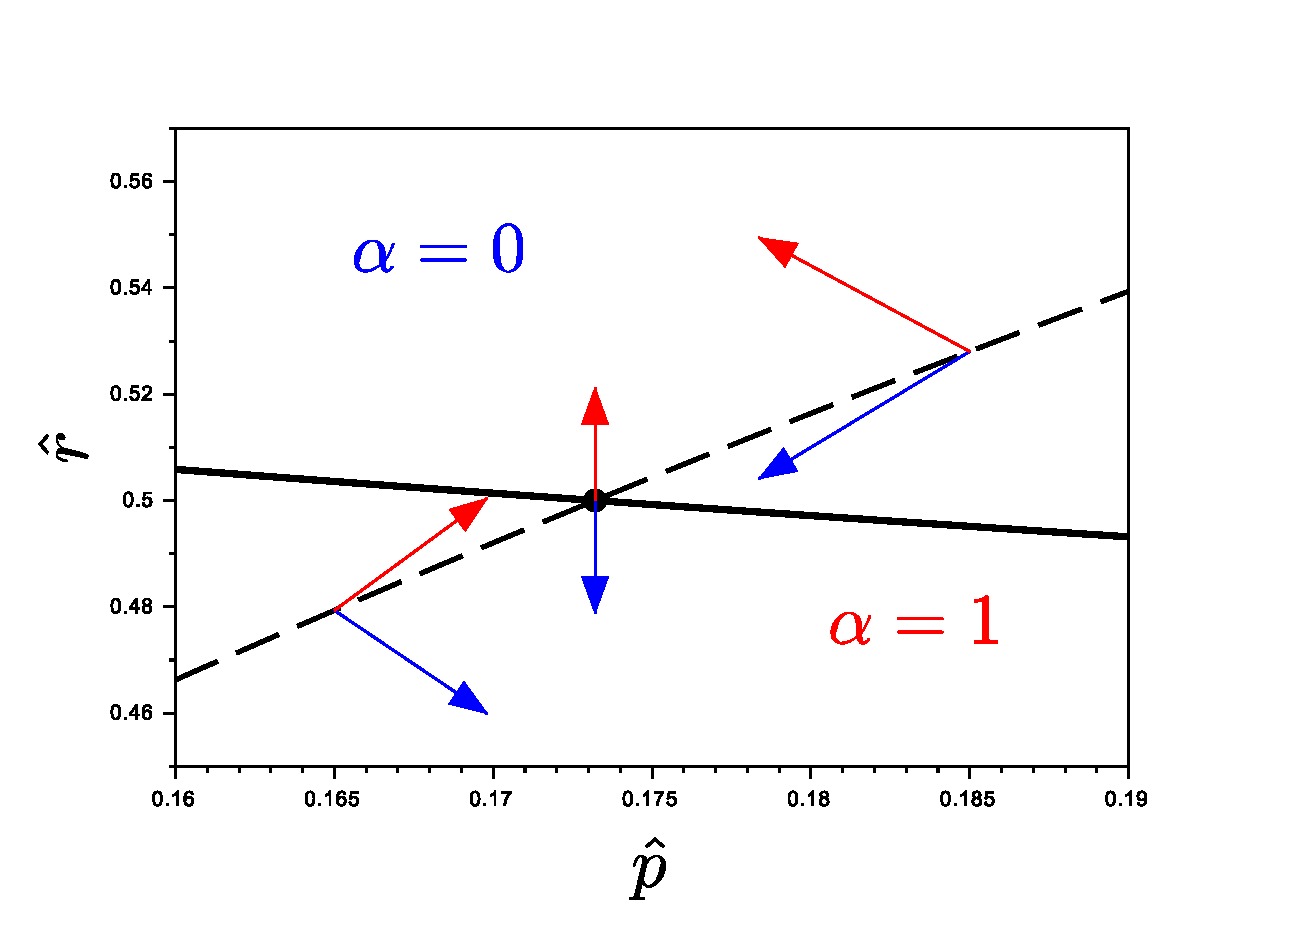
\includegraphics[width=0.8\textwidth]{Fig/Fig_sliding}
\caption
{
\textbf{Local stability of the on-off strategy.}
The on-off strategy sets $\alpha$ to a value of 0 (1) when $\hat{r} > g(\hat{p})$ ($\hat{r} < g(\hat{p})$).
The solid, black curve is the $\hat{p}$-nullcline.
The dashed, black curve is the curve $\hat{r}=g(\hat{p})$.
The arrows represent the vector fields for $\alpha=0$ (in blue) and $\alpha=1$ (in red).
The intersection of the $\hat{p}$-nullcline and the curve $\hat{r}=g(\hat{p})$ corresponds to a unique non-trivial stable steady state, which is equal to $(\hat{p}_{opt}^*, \hat{r}_{opt}^*)$ by Eq.~\ref{eq:supp_adim_h}.
}
\label{fig:sliding}
\end{figure}

\clearpage

\subsection{S2 Text -- Model parameters}
\manuallabel{S2_Text}{S2~Text}

Most of the conclusions of this paper are parameter-independent in the range of physically admissible values.
The exact parameter values used in the simulations aim to represent relevant orders of magnitude.
They were derived from the available literature on fast-growing bacteria (mostly \textit{Escherichia coli}).
This document describes this derivation for each parameter.
In the \textit{Methods} section of the main text, we also describe how some of them were validated by fitting the model to available experimental data (Fig.~\ref{fig:model_validation} in the main text).

The model parameters (Eqs.~\ref{eq:pdef}-\ref{eq:rdef} in the main text) are listed in the table below:
\begin{center}
\begin{tabular}{|c|c|l|}
\hline
Name & Unit & Description \\
\hline
$e_M$ & h$^{-1}$ & Constant characterizing nutrient composition of medium\\
\hline
$k_R$ & h$^{-1}$ & Rate constant of macromolecular synthesis\\
\hline
$K_R$ & g\ L$^{-1}$ & Half-saturation constant of macromolecular synthesis\\
\hline
$\beta$ & L\ g$^{-1}$ & Inverse of the cellular density of macromolecules\\
\hline
$\alpha$ & -- & Resource allocation parameter\\
\hline
\end{tabular}
\end{center}
The values derived below are summarized in \ref{S1_Table}.


\subsubsection{\Large \texorpdfstring{$e_M$}{eM}}

By definition, $e_M$ is the effective turnover of the metabolic macroreaction producing precursors from external substrates, obtained by dividing the reaction rate $v_M$ by the enzyme concentration $m$ (Eq.~\ref{eq:metaflux}).
The unit of $e_M$ is min$^{-1}$, and can be decomposed as follows:
\[
[e_M]  = \frac{\text{[mass of metabolic product]}}{\text{[mass of enzyme M]}\cdot \text{[time]}} = \frac{1}{\text{[time]}}.
\]
Note that $e_M = k_M\, s / (K_M + s)$ where $k_M$ is a rate constant, indicating the maximal rate of conversion of external nutrients to precursor metabolites. 
$e_M$ will thus vary with the concentration $s$ of the external nutrients and the kind of nutrient. 
For example, the precursor mass that can be produced from 1 g of glucose is higher than that produced from 1 g of acetate.

How can we find a typical value for $k_M$, and thus for $e_M$ (both have the same order of magnitude if we suppose that the reaction is not operating far below saturation, that is, $e_M \approx k_M$)?
A reasonable estimate for $k_M$ can be obtained from the turnover numbers of reactions involved in the synthesis of charged tRNA, since the latter are directly consumed by the most abundant part of the gene expression machinery, the ribosomes.

Ref.~\cite{uter_longrange_2004} provides a typical value for such a reaction, catalyzed by glutaminyl-tRNA synthetase: $k_{\textit{cat,GlnRS}} = 3.2$~s\textsuperscript{-1}, indicating that on average 3.2 glutaminyl-tRNA molecules are produced per glutaminyl-tRNA synthetase molecule per second. 
After conversion to mass units using molar weight from~\cite{freist_glutaminyltrna_1997}, this yields
\[
k_{\textit{cat,GlnRS}} = \frac{3.2 \cdot 147}{64.4 \cdot 10^ 3} \approx 10^{-3} \, \text{g of glutaminyl-tRNA} \cdot \text{g of enzyme}^{-1} \cdot \text{s}^{-1}.
\]
We therefore take
\[
k_M \approx 3.6 \text{ h}^{-1},
\]
and thus obtain an upper bound for $e_M$ in our simulations.

\subsubsection{\Large \texorpdfstring{$k_R$}{kR}}

$k_R$ is the mass rate constant describing the maximal rate of conversion of precursors to macromolecules [h\textsuperscript{-1}].
As for $e_M$, we can decompose this into
\[
[k_R]  = \frac{\text{[mass of macromolecules]}}{\text{[mass of gene expression machinery]}\cdot \text{[time]}} = \frac{1}{\text{[time]}}
\]
To obtain an order of magnitude for the mass of macromolecules, we focus on proteins since they are the most abundant macromolecules in the cell~\cite{ehrenberg_mediumdependent_2012}.
The dimensional analysis of $k_R$ thus becomes:
\[
\begin{aligned}
\left[k_R\right] &= \frac{\text{[protein mass produced]}}{\text{[ribosomal mass]} \cdot \text{[hour]}}\\
&= \frac{\text{[moles of protein]} \cdot \text{[protein molar mass]}}{\text{[moles of ribosome]} \cdot \text{[ribosome molar mass]} \cdot \text{[hour]}}\\
&= \frac{\text{[moles of amino acids]} \cdot \text{[molar mass of amino acids]}}{\text{[moles of ribosome]} \cdot \text{[hour]} \cdot \text{[ribosome molar mass]}}\\
&\approx \frac{\text{[maximal protein elongation rate]} \cdot \text{[molar mass of amino-acids]}}{\text{[ribosome molar mass]}}.
\end{aligned}
\]
The values in the last equality are available from the literature~\cite{ehrenberg_mediumdependent_2012,klumpp_molecular_2013,hachiya_increase_2007,yamamoto_mass_2006}.
We obtain
\[
k_R \approx \frac{10 \cdot 100}{10^6}\cdot 3600 \approx 3.6 \text{ h}^{-1}.
\]
This value is comparable with the translational capacity $k_T$, in $\mu$g of protein per $\mu$g of ribosomal protein per hour, given by Scott \textit{et al.}~\cite{scott_interdependence_2010}:
\[
k_T = \frac{4.5 \text{ }\mu\text{g of protein} \text{ / }\mu\text{g of RNA} \text{ / h }}{0.76 \text{ }\mu\text{g of ribosomal protein} \text{ / } \mu\text{g of RNA}} = 5.9 \text{ h}^{-1}.
\]

\subsubsection{\Large \texorpdfstring{$K_R$}{KR}}

A value for the parameter $K_R$, representing the half-saturation constant of macromolecular synthesis, is more difficult to obtain from the literature.
However, assuming that ribosomes operate close to saturation (80\% over a range of growth rates~\cite{ehrenberg_mediumdependent_2012}), we find that $K_R \approx 0.25\,p$, with p the total amino acid concentration.
The total concentration of amino acids in the cell is around 150~mmol~L\textsuperscript{-1}~\cite{bennett_absolute_2009}, which with a mean molecular weight of 118.9~g~mol\textsuperscript{-1} for amino acids~\cite{hachiya_increase_2007}, yields a mass concentration of 17.8~g~L\textsuperscript{-1}.
These considerations led to the following order of magnitude for $K_R$:
\[
K_R \approx 1\text{ g L}^{-1}.
\]

\subsubsection{\Large \texorpdfstring{$\beta$}{Beta}}

$\beta$ is the inverse of the cellular density of macromolecules, which has been shown constant during balanced growth over a large range of growth rates~\cite{churchward_macromolecular_1982}, and there is some data suggesting that $\beta$ varies little during growth transitions as well~\cite{zhou_carbon_2013}.
From~\cite{zimmerman_estimation_1991,mcguffee_diffusion_2010} we take the following typical value for $\beta$:
\[
\beta \approx \frac{1}{300} \approx 0.003 \text{ L g}^{-1}.
\]

\subsubsection{\Large \texorpdfstring{$E_M$}{EM} and \texorpdfstring{$K$}{K}}

From the values of the parameter in the dimensional model, one can deduce the parameters in the nondimensional model used in the simulations:
\[
E_M = \frac{e_M}{k_R} = \frac{3.6}{3.6} = 1 \;\;\;\;\; , \;\;\;\;\;  K = \beta\, K_R = 3\cdot 10^{-3} \cdot 1 = 0.003.
\]

\clearpage

\subsection{S3 Text -- Solution of optimal control problem}
\manuallabel{S3_Text}{S3~Text}

\subsubsection{Statement of the problem}

We consider the dimensionless system defined by Eqs~\ref{eq:pdefnondim}-\ref{eq:rdefnondim} in the main text, which are here repeated for clarity:
\begin{equation}{\label{eq:model}}
\begin{aligned}
\frac{d\hat{p}}{d\hat{t}} &= (1-\hat{r})\, E_M - (1+\hat{p})\, \hat{r} \, \frac{\hat{p}}{K+\hat{p}}, \\
\frac{d\hat{r}}{d\hat{t}} &= \hat{r} \frac{\hat{p}}{K + \hat{p}} \, (\alpha (\hat{t}) - \hat{r}).
\end{aligned}
\end{equation}

As stated in the section \textit{Biomass maximization as an optimal control problem} in the main text, the objective of this study is to maximize the growth rate on an interval $[0,\tau]$ after a nutrient upshift. With Eq.~\ref{S1.eq:supp_growthrate_adim} in \ref{S1_Text}, we have
 
\begin{equation*}
\hat{\mu}= \hat{r}\, \dfrac{\hat{p}}{K+\hat{p}}.
\end{equation*}
In order to avoid boundary effects occurring over finite time intervals, notably the depletion of precursors just before $\tau$, we solve the optimal control problem over an infinite horizon ($\tau \rightarrow \infty$). Consider the set of admissible controls
\[
\mathcal{U}=\{\alpha:\mathbb{R} \rightarrow [0,1] \ \mid \ \alpha(\cdot) \ \mathrm{measurable}\}.
\]
The optimization problem can then be stated as follows:
\begin{equation}\label{Prob}
\alpha_{opt} = \arg \max_{\alpha \in \mathcal{U}} J(\alpha)\equiv \int_0^{+\infty} \hat{r}(\hat{t}) \frac{\hat{p}(\hat{t})}{K + \hat{p}(\hat{t})} d\hat{t} ,
\end{equation}
where $(\hat{p}(\hat{t}),\hat{r}(\hat{t}))$ is the unique solution of Eq.~\ref{eq:model} starting at a given point $(\hat{p}_0,\hat{r}_0)\in \Omega \equiv \mathbb{R}^+_* \times (0,1)$ for a given control $\alpha\in \mathcal{U}$.

Given that the performance index $J(\alpha)$ diverges, we actually consider \textit{overtaking optimality}~\cite{carlson_infinite_1991}.
Consider the performance index of the trajectory $x(\cdot)$ emanating from $x_0$ and generated by $u(\cdot)$ defined for any $T\geq 0$ by
$$
J_T(x_0,u(\cdot))=\int_0^T f_0(x(t),u(t),t)dt.
$$
A trajectory $x^*(\cdot)$ emanating from $x_0$ and generated by $u^*(\cdot)$ is said to be overtaking optimal if for any other trajectory $x(\cdot)$ emanating from $x_0$ and generated by $u(\cdot)$ the following holds
$$
\liminf_{T\rightarrow\infty} \left\lbrace J_T(x_0,u^*(\cdot)) - J_T(x_0,u(\cdot))\right\rbrace\geq 0.
$$
Roughly speaking, a trajectory is overtaking optimal if "the performance index catches up with the performance index of any other trajectory"~\cite{carlson_infinite_1991}.

\subsubsection{Maximum Principle}

Necessary conditions on optimal trajectories can be obtained by the Infinite Horizon Maximum Principle~\cite{carlson_infinite_1991}.
Let $H(\hat{p},\hat{r},\lambda_p,\lambda_r,\lambda_0,\alpha)$ be the Hamiltonian of the system, defined by
\[
H(\cdot) \equiv \lambda_p\, E_M\, (1-\hat{r}) - \hat{r}\, \dfrac{\hat{p}}{K+\hat{p}}\left[\lambda_p (1+\hat{p}) +\lambda_r\, \hat{r} +\lambda_0\right] + \alpha \, \lambda_r \, \hat{r}\, \frac{\hat{p}}{K+\hat{p}}.
\]
Moreover, let $\alpha$ be an optimal control, and $\hat{x}(\cdot)=(\hat{p}(\cdot),\hat{r}(\cdot))$ the associated trajectory.
Then, there exists $\lambda_0 \leq 0$ and an absolutely continuous map $\lambda=(\lambda_p,\lambda_r):[0,+\infty) \rightarrow \mathbb{R}^2$
such that $(\lambda,\lambda_0)\neq0$, and
\begin{align}
\dot{\lambda}_p\, =-\frac{\partial H}{\partial \hat p}&= \hat{r} \, \frac{K}{(K+\hat{p})^2}\, \left[\lambda_p \, (1+\hat{p}) +\lambda_r\, ( \hat{r}-\alpha) + \lambda_0\right] + \hat{r}\, \frac{\hat{p}}{K+\hat{p}}\, \lambda_p, \label{eq:adjoint_p}\\
 \dot{\lambda}_r\, =-\frac{\partial H}{\partial \hat r}&= \lambda_p\, E_M +\frac{\hat{p}}{K+\hat{p}} \, \left[\lambda_p \, (1+\hat{p}) +\lambda_r\, (2 \hat{r}-\alpha) +\lambda_0\right] \label{eq:adjoint_r}.
\end{align}
The maximization condition is given by:
\begin{equation}{\label{eq:PMP}}
\begin{aligned}
&\alpha(\hat{t}) \in \arg\ max_{v \in [0,1]} H(\hat{x}(\hat{t}),\lambda(\hat{t}),\lambda_0,v), \\ &\mathrm{almost}\ \mathrm{everywhere}\ \mathrm{on}\ [0,+\infty).
\end{aligned}
\end{equation}

An extremal trajectory is a quadruplet $(\hat{x}(\cdot),\lambda(\cdot),\lambda_0,\alpha(\cdot))$ satisfying Eqs~\ref{eq:model}-\ref{eq:PMP}. The extremal is said to be normal (resp. abnormal) if $\lambda_0<0$ (resp. $\lambda_0=0$). In the normal case, we normalize the adjoint vector so that $\lambda_0=-1$.\\

From Eq.~\ref{eq:PMP}, it follows that the control strategy is given by the sign of the \textit{switching function} $\phi(\cdot) \equiv \lambda_r \, \hat{r}\, \hat{p}/(K+\hat{p})$, that is,
\[
\begin{cases}
\alpha=1 \iff \phi(\cdot) >0,\\
\alpha=0 \iff \phi(\cdot)<0.
\end{cases}
\]

Finally, given that the system is autonomous, the Hamiltonian is conserved along any extremal trajectory.

\subsubsection{Characterization of singular arcs}

Whenever $\phi$ is vanishing over a time interval, we say that the trajectory is \textit{singular}.
We will now characterize such trajectories.
If $I=[\hat{t}_1,\hat{t}_2]$ is a singular arc, we have $\phi(\hat{t})=\dot{\phi}(\hat{t})=0$, for all $\hat{t}\in[\hat{t}_1,\hat{t}_2]$, that is, $\lambda_r(\hat{t})=0$ and $\dot\lambda_r(\hat{t})=0$. 

For abnormal extremal trajectories, we get $\lambda_p(\hat{t})=0$, in contradiction with the Maximum Principle, so there is no singular arc. An abnormal extremal trajectory is therefore a concatenation of bang arcs.

For normal extremal trajectories, using additionally that $H$ is constant along an extremal trajectory, we obtain that $\lambda_p$ is constant along a singular arc. By combining $\dot \lambda_p=0$ and $\dot \lambda_r=0$, we obtain $\hat{p}(\hat{t})=\sqrt{E_M\, K}=\hat{p}_{opt}^*$. Using $d\hat{p}/d\hat{t}=0$, we finally get $\hat{r}(\hat{t})=\hat{r}_{opt}^*$.
Thus, the singular arc is the optimal steady state, corresponding to a singular control $\alpha(\hat{t})=\alpha_{opt}^*$, with $\alpha_{opt}^*$ depending on $E_M$ (\ref{S1_Text}).

A necessary condition of optimality for a singular arc is given by the Kelley condition~\cite{borisov_fullers_2000}.
We must differentiate $\phi$ with respect to $\hat{t}$ until $\alpha$ appears in the derivative. Along a singular arc, we obtain for $q=2$:
$$
(-1)^q\frac{\partial}{\partial\alpha}\frac{d^{2q}}{d\hat{t}^{2q}}\phi(\hat{t})<0,
$$
satisfying the Kelley condition necessary for optimality. Given that the singular arc is of second order, an optimal trajectory can enter into the singular arc only by a \textit{chattering arc} (also called the Fuller's phenomenon, \textit{i.e.}, an arc with an infinite number of switches~\cite{borisov_fullers_2000,marchal_chattering_2013}). \\


\subsubsection{Analysis of the adjoint system}

Recalling that a switch corresponds to a change of sign of $\lambda_r$, the analysis of the adjoint system (Eqs~\ref{eq:adjoint_p}-\ref{eq:adjoint_r}) may be useful to characterize the switches of extremal trajectories. 

First, for the abnormal case, we can easily determine in the phase-plane the possible transitions between the four regions defined by the axes (see Fig.~\ref{fig-adj}). A trajectory can cross at most twice the $\lambda_p$-axis, so  we conclude that an abnormal extremal cannot have more than two switches. Thus, an abnormal extremal is a concatenation of at most three bang arcs ($\alpha(t)=0$ or $\alpha(t)=1$). When  $\alpha(t)=0$ or $\alpha(t)=1$ for a long time, the growth rate tends to zero. We therefore conclude that  abnormal extremal trajectories are not optimal.

Secondly, for the normal case, after the first switch, a trajectory with two consecutive switches in the regions $\{(\hat{p},\hat{r})\in \Omega \mid \hat{p}<\hat{p}_{opt}^*\}$ or $\{(\hat{p},\hat{r})\in \Omega \mid \hat{p}>\hat{p}_{opt}^*\}$ is not possible, as shown in Fig.~\ref{fig-adj}. Therefore, such a trajectory is not optimal given that it does not fulfill the conditions given by the Maximum Principle.
We conclude that if the optimal trajectory has a concatenation of bang arcs, the switches must alternatingly occur in the regions  $\{(\hat{p},\hat{r})\in \Omega \mid \hat{p}<\hat{p}_{opt}^*\}$ and $\{(\hat{p},\hat{r})\in \Omega \mid \hat{p}>\hat{p}_{opt}^*\}$.

\begin{figure}[tb]
\centering
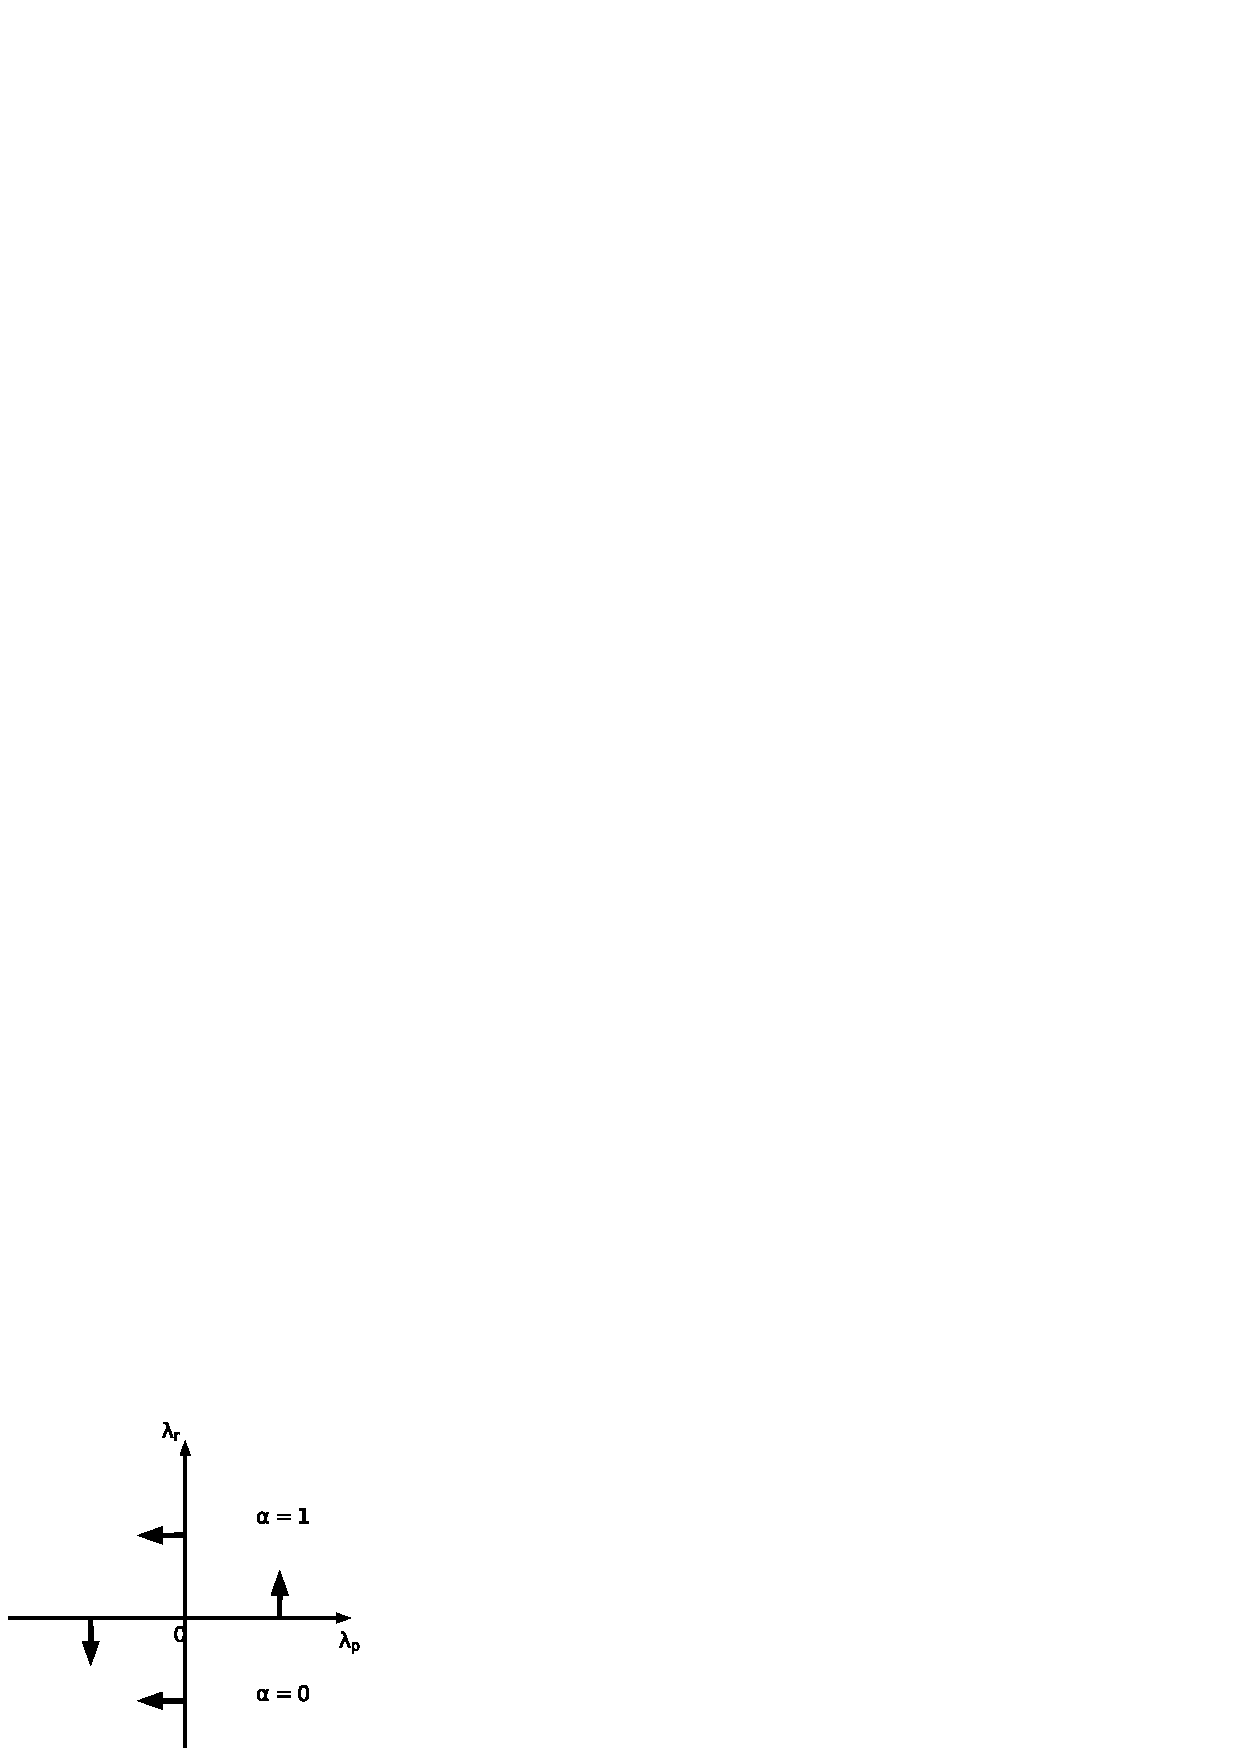
\includegraphics[height=4cm]{Fig/adj2ab} 
\includegraphics[height=4cm]{Fig/adj2} 
\caption{\textbf{Transitions between regions in the phase-plane for the adjoint system.} A switch occurs when a trajectory crosses the $\lambda_p$-axis. Left: abnormal case. An extremal trajectory cannot have more than two switches. Right: normal case. $(\lambda_p^s,0)$ corresponds to the singular arc.  After the first switch, an extremal trajectory cannot have two consecutive switches if it stays in the region $\{(\hat{p},\hat{r})\in \Omega \mid \hat{p}<\hat{p}_{opt}^*\}$ or $\{(\hat{p},\hat{r})\in \Omega \mid \hat{p}>\hat{p}_{opt}^*\}$.}
\label{fig-adj}                               
\end{figure} 


\subsubsection{Optimal trajectories}

From the Maximum Principle, we have shown that the optimal trajectory is a concatenation of bang arcs ($\alpha(t)=0$ or $\alpha(t)=1$) and possibly a singular arc corresponding to the optimal steady state $(\hat{p}(\hat{t}),\hat{r}(\hat{t}))=(\hat{p}_{opt}^*,\hat{r}_{opt}^*)$. Moreover, if the optimal trajectory has a singular arc, it must enter it through a chattering arc (\textit{i.e.}, with an infinite number of switches between $\alpha=0$ and $\alpha=1$).

These elements motivate the supposition that optimal solutions consist in a transient (chattering arc) towards the optimal steady state, after which they remain there (until the next change of environment). The chattering arc can be characterized by a switching curve $\hat{p}\mapsto\varphi(\hat{p})$ which passes through the optimal steady state.
Defining $A_0$ and $A_1$ the regions above and below $\varphi$ in the $(\hat{p},\hat{r})$-plane, respectively, we conjecture that the following feedback control law is optimal: 
%The simplest way to reach the optimal steady-state is thus two arcs, either 0-1 or 1-0 depending on the initial conditions. More precisely, let $\phi_0$ and $\phi_1$ be defined as the the trajectories solution of System \eqref{model} backward in time starting at $(p_{opt}^*,r_{opt}^*)$ with respectively $\alpha=0$ and $\alpha=1$. Given $\phi=\phi_0 \cup \phi_1$, we define $A_0$ and $A_1$ the regions above and below $\phi$ in the plane $(p,r)$. 


\begin{equation}\label{control-opt}
\begin{cases}
\alpha(\hat{t})=0 \ \textrm{if} \ (\hat{p}(\hat{t}),\hat{r}(\hat{t}))\in A_0,\\
\alpha(\hat{t})=1 \ \textrm{if} \ (\hat{p}(\hat{t}),\hat{r}(\hat{t}))\in A_1,\\
\alpha(\hat{t})=\alpha_{opt} \ \textrm{if} \ (\hat{p}(\hat{t}),\hat{r}(\hat{t}))=(\hat{p}_{opt}^*,\hat{r}_{opt}^*).
\end{cases}
\end{equation}


Loosely speaking, the chattering arc corresponds to a spiral composed of bang arcs wrapping around the optimal steady state, where the switches alternatingly occur in the regions  $\{(\hat{p},\hat{r})\in \Omega \mid \hat{p}<\hat{p}_{opt}^*\}$ and $\{(\hat{p},\hat{r})\in \Omega \mid \hat{p}>\hat{p}_{opt}^*\}$, in line with the analysis of the adjoint system.
This is a first hint that the proposed control strategy is optimal. Moreover, our conjecture is also in line with the \textit{turnpike property}:
Trélat and Zuazua~\cite{trelat_turnpike_2015} have shown that, for quite a generic class of systems, the optimal strategy consists in staying at the optimal steady state (after a short transient).

As explained in the \textit{Methods} section of the main text, we numerically solved the optimal control problem by the direct method using the \texttt{bocop} software~\cite{bonnans_bocop_2012}. 
It is important to stress that the optimization process was performed without any preliminary assumptions on the characteristics of the optimal trajectory. 
The fact that the numerical solution verifies the Maximum Principle (\textit{i.e.}, the singular arc corresponds to the optimal steady state) and the Kelley condition (\textit{i.e.}, the presence of a chattering arc)
tends to confirm that the control strategy of Eq.~\ref{control-opt} is optimal. As an aside, we note that due to the fact that numerical optimization was performed for a finite horizon, we actually obtained a second chattering arc escaping from the singular arc at the end of the simulation.  This is a classical property of the turnpike strategy: the optimal trajectory leaves the optimal steady state just before the end of the time interval of interest, in our case consuming almost all precursors. This arc was removed from the plot in Fig.~\ref{fig:optimalcontrol}, because it does not occur with an infinite horizon and is therefore a numerical artifact for this study.

\clearpage

\subsection[S4 Text -- Kinetic model of the ppGpp system]{S4 Text -- Kinetic model of the ppGpp system in \textit{Escherichia coli}}
\sectionmark{Kinetic model of the ppGpp system}
\manuallabel{S4_Text}{S4~Text}

The recently published model of Bosdriesz \textit{et al.}~\cite{bosdriesz_how_2015} provides a synthesis of the currently available knowledge of the ppGpp regulatory system.
Through the mechanisms of ppGpp production and degradation, it describes regulation of the synthesis of ribosomal RNA.
We explain below how we use the model to compare the action of the ppGpp system with the on-off control strategy.
The denomination of variables and parameters follows the Supporting Information of~\cite{bosdriesz_how_2015} , and is reproduced in Table~\ref{S4.tab:notations} in order to make the text self-contained.

The evolution of the cellular concentration of ppGpp is described in~\cite{bosdriesz_how_2015} by
\begin{equation}
\label{eq:ppGpp}
\frac{d\texttt{ppGpp}}{dt} = v_{RelA}(r_{t,tot}) + v_{spoT} - k_{spoT} \cdot \texttt{ppGpp},
\end{equation}
where $v_{spoT}$ and $k_{spoT}$ are constants (see Table~\ref{S4.tab:notations}), and $v_{RelA}$ is a function of $r_{t,tot}$, the total concentration of "stalled" ribosomes:
\begin{equation}
\label{eq:vrelA}
v_{RelA}(r_{t,tot}) = k_{RelA} \cdot RelA_{tot} \cdot \frac{r_{t,tot}}{K_{D,RelA} + r_{t,tot}}.
\end{equation}
The amount of stalled ribosomes is determined by the equilibrium between charged and uncharged tRNA, $t_{ai}$ and $t_{i}$, in the cell:
\begin{equation}
\label{eq:rttot}
r_{t,tot} = \sum_i r_{ti} = \sum_i r_i \frac{t_i/\kappa_{t}}{1+t_{ai}/\kappa_{ta}+t_i/\kappa_{t}},
\end{equation}
which can be rewritten as
\begin{equation}
\label{eq:rttot-f}
r_{t,tot} = \sum_i r_i \frac{t_i/\kappa_{t}}{1+(0.5 r-t_i)/\kappa_{ta}+t_i/\kappa_{t}},
\end{equation}
using the assumption that $t_{tot,i}  = t_{ai} + t_i = 0.5 \cdot r$.
$r_i$ denotes the concentration of ribosomes recognizing amino acid  $i$.
Finally, with $r = \sum_i r_i$ the total ribosome concentration and $a_i$ the concentration of amino acid $i$, the dynamics of the charged tRNA concentration is described by
\begin{equation}
\label{eq:ti_dynamic}
\frac{dt_{ai}}{dt} = v_{tai}(a_i, t_{i}) - f_i \cdot v_{ribosome}(t_i,r),
\end{equation}
with $v_{tai}(a_i, t_{i})$ the synthesis rate of charged tRNA, and $f_i \cdot v_{ribosome}(t_i,r)$ their consumption via protein synthesis.
In particular,
\begin{eqnarray}
v_{tai}(a_i, t_{i}) &=& k_{Si} \cdot S_{tot,i} \cdot \frac{t_i\, a_i}{t_i\,  K_{Mai} + a_i\,  K_{Mti} + t_i\,  a_i}, \label{eq:vtai}\\
v_{ribosome}(t_i, r) &=& k_{rib} \cdot r \cdot \left(1+ \sum_i \left[ f_i \cdot \left( 1 + \frac{t_i}{\kappa_t} \right) \frac{\kappa_{ta}}{0.5\cdot r - t_i} \right]\right)^{-1}. \label{eq:vrib}
\end{eqnarray}

For comparison with our framework, we need $\texttt{ppGpp}$ as a direct function of the total amino acid concentration $a = \sum_i a_i$ (a proxy for precursors) and total ribosome concentration $r$ (a proxy for gene expression machinery).
To this end, we made two additionnal assumptions:
\begin{description}
\item[(A1)] All concentrations specific to one type of amino acid $i$ ($a_i$, $t_{ai}$, $t_{i}$, $r_i$) are in the same proportion $f_i = f = 1/20$ with respect to the total concentrations ($a$, $t_{a}$, $t$, $r$).
\item[(A2)] We apply a quasi-steady-state approximation (QSSA) to the dynamics of the concentration of the charged tRNAs ($t_{ai}$) and the concentration of ppGpp ($\texttt{ppGpp}$).
That is, the dynamics of these variables are assumed fast relative to the dynamics of the amino acid concentrations ($a_i$) and the total ribosome concentration ($r$).
\end{description}
Using (A2), we can rewrite Eq.~\ref{eq:ti_dynamic} as follow:
\begin{equation}\label{eq:vtai_vrib}
v_{tai}(a_i, t_{i}) = f_i \cdot v_{ribosome}(t_i,r),
\end{equation}
which, using (A1) and Eqs~\ref{eq:vtai} and \ref{eq:vrib}, leads to:
\begin{equation}
\label{eq:vtai_vrib_without_sum}
k_{Si} \cdot S_{tot,i} \cdot \frac{t_i\, a_i}{t_i\, K_{Mai} + a_i\, K_{Mti} + t_i\, a_i}
= f_i \cdot k_{rib} \cdot r \cdot
  \left(1 + \frac{\kappa_{ta}}{0.5 r - t_i} \cdot \left( 1 + \frac{t_i}{\kappa_t} \right)  \right)^{-1}.
\end{equation}
By rearranging both sides of the equation, $t_i$ can be expressed as a function of $a_i$ and $r$, which yields:

\begin{equation}
\begin{alignedat}{2}
&A {t_i}^2 + B t_i + C = 0, \;\;\; \text{with}\\
&A = \frac{k_{Si} \,S_{tot,i} \,a_i}{f_i\, k_{rib} \,r} \left( \frac{\kappa_{ta}}{\kappa_t} - 1\right) + K_{Mai} + a_i,\\
&B = \frac{k_{Si} \,S_{tot,i} \,a_i}{f_i \,k_{rib} \,r} (0.5\,r+\kappa_{ta}) + a_i \,K_{Mti} - 0.5\,r\,(K_{Mai} + a_i),\\
&C = - 0.5 \,r \,a_i \,K_{Mti},
\end{alignedat}
\end{equation}
and therefore
\[
t_i (a_i, r) = \frac{-B \pm \sqrt{B^2 - 4AC}}{2A}.
\]
It is not difficult to show that the only solution on $[0, 0.5\,r]$ is
\begin{equation}
\label{eq:ti_final}
t_i (a_i, r) = \frac{-B + \sqrt{B^2 - 4AC}}{2A}.
\end{equation}
From this result, we obtain $r_{t,tot}$ as a function of $a_i$ and $r$, by applying (A1) to Eq.~\ref{S4.eq:rttot-f}:
\begin{equation}
\label{eq:rttot-f_without_sum}
r_{t,tot}(t_i, r) = r \cdot \frac{t_i/\kappa_{t}}{1+(0.5 r-t_i)/\kappa_{ta}+t_i/\kappa_{t}},
\end{equation}
and substituting $t_i$ by the expression of Eq.~\ref{eq:ti_final}.

Finally, we apply (A2) to Eq.~\ref{eq:ppGpp} and obtain the final expression giving the concentration of ppGpp as a function of the total amino acid and ribosome concentrations:
\begin{equation}
\footnotesize
\texttt{ppGpp}(a_i, r) = \frac{1}{k_{spoT}} \left( k_{RelA} \cdot RelA_{tot} \cdot \frac{r_{t,tot}(a_i, r)}{K_{D,RelA} + r_{t,tot}(a_i,r)} + v_{spoT} \right).
\end{equation}
This function is represented in Fig.~\ref{S4.fig:ppGpp} with parameters taken from Table~\ref{tab:notations}.

The plotted surface of the function resembles the inverse of the on-off control strategy in Fig.~\ref{fig:ppGppsurface}, as expected, bearing in mind that ppGpp has an inhibitory effect on the synthesis of ribosomal RNA.
We assumed a Michaelis-Menten inhibition for the regulatory effect of ppGpp on rRNA synthesis, and thus indirectly on the synthesis of ribosomal proteins~\cite{potrykus_pppgpp_2008,keener_regulation_1996}:
\begin{equation}
\alpha (\texttt{ppGpp}) = \frac{K_I}{K_I + \texttt{ppGpp}}.
\end{equation}
The inhibitory constant $K_I$ lies in the dynamical range of variation of $\texttt{ppGpp}$.
In Fig.~\ref{fig:ppGppsurface} in the main text, we took $K_I = 10$~$\mu$M.

\begin{figure}[tb]~Text
\centering
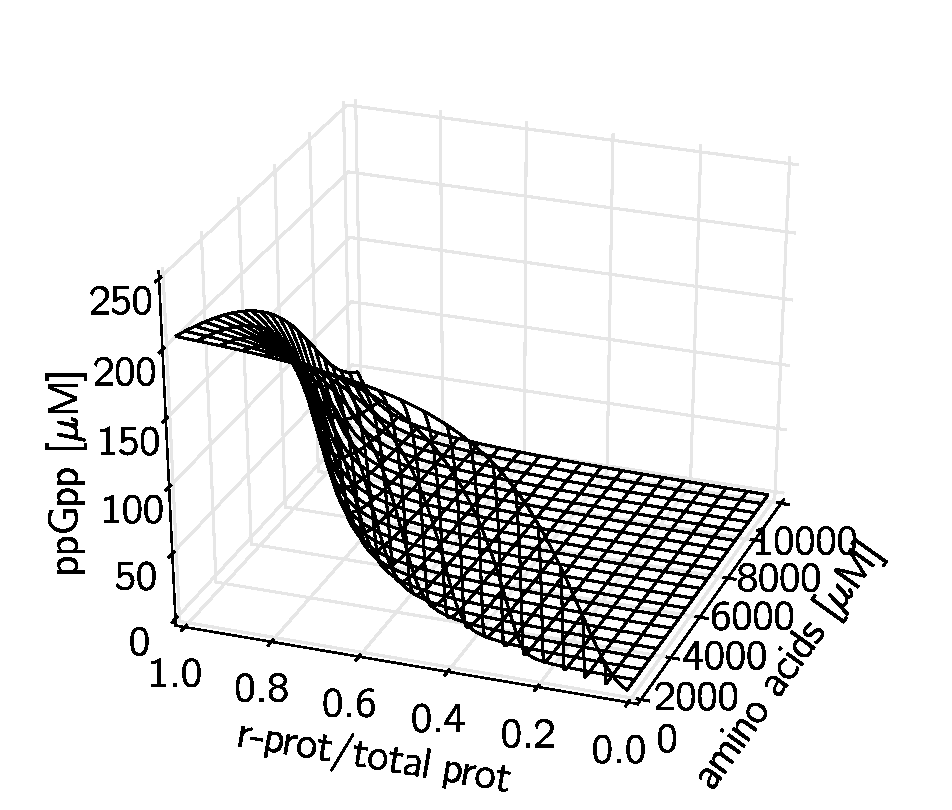
\includegraphics[width=0.7\textwidth]{./Fig/FigS4-1}
\caption[ppGpp concentration is a function of total ribosome and amino acid concentrations.]
{
{\bf ppGpp concentration is a function of total ribosome and amino acid concentrations.}\newline
We assume the dynamics of ppGpp to be fast on the time-scale of changes in the ribosome and amino acid concentrations.
The concentration of ppGpp can thus be expressed as a function of the latter two variables, using the model of Bosdriesz \textit{et al.}~\cite{bosdriesz_how_2015}.
Parameters are taken from Table~\ref{tab:notations}.
}
\label{fig:ppGpp}
\end{figure}

\begin{table}[tb]
\scriptsize
\centering
\begin{tabular}{cccl}
\hline
\hline
\textbf{Symbol} & \textbf{Value} & \textbf{Unit} & \textbf{Description} \\
\hline
\hline
$a_i$ & -- & $\mu$M & Concentration of aa $i$ (not incorporated in protein)\\

$t_{ai}$ & -- & $\mu$M & Concentration of tRNA charged with aa $i$\\

$t_{i}$ & -- & $\mu$M & Concentration of free tRNA conjugate to aa $i$\\

$t_{tot,i}$ &  $0.5 \cdot r$ & $\mu$M & Total concentration of tRNA conjugate to aa $i$\\

$r_{i}$ & -- & $\mu$M & Total concentration of ribosome with an A-site for aa $i$\\

$r_{ti}$ & -- & $\mu$M & Ribosomes with uncharged tRNA in an A-site for aa $i$\\

$\texttt{ppGpp}$ & -- & $\mu$M & Concentration of ppGpp\\
\hline
$a$ & $\sum_i a_{i}$ & $\mu$M & Total concentration of aa (not incorporated in protein)\\

$t_{a}$ & $\sum_i t_{ai}$ & $\mu$M & Total concentration of tRNA charged with aa\\

$t$ & $\sum_i t_{i}$ & $\mu$M & Total concentration of free tRNA\\

$r_{t,tot}$ & $\sum_i r_{ti}$ & $\mu$M & Total concentration of uncharged tRNA bound to ribosomes\\

$r$ & $\sum_i r_i$ & $\mu$M & Total concentration of ribosomes\\
\hline
$v_{RelA}$ & -- & $\mu$M/s & Rate of RelA-catalyzed ppGpp synthesis\\

$v_{SpoT}$ & $10^{-3}$ & $\mu$M/s & Rate of ppGpp synthesis by SpoT\\

$v_{tai}$ & -- & $\mu$M/s & Rate of amino-acyl tRNA $i$ synthetase\\

$v_{ribosome}$ & -- & $\mu$M/s & Total rate of protein synthesis\\
\hline
$k_{rib}$ & 20 & s\textsuperscript{-1} & $k_{cat}$ of protein elongation\\

$k_{RelA}$ & 75 & s\textsuperscript{-1} & $k_{cat}$ of ppGpp synthesis by RelA\\

$K_{D,RelA}$ & 0.26 & $\mu$M & Michaelis constant of RelA-catalyzed ppGpp production\\

$RelA_{tot}$ & 1/15 & $\mu$M & RelA concentration\\

$k_{SpoT}$ & $\ln (2) / 30$ & s\textsuperscript{-1} & Rate of ppGpp degradation by SpoT\\

$\kappa_t$ & 500 & $\mu$M & Dissociation constant of uncharged tRNA-ribosome complex\\

$\kappa_{ta}$ & 1 & $\mu$M & Dissociation constant of charged tRNA-ribosome complex\\

$k_{Si}$ & 100 & s\textsuperscript{-1} & $k_{cat}$ of aminoacyl-tRNA synthetase\\

$S_{tot,i}$ & 1 & $\mu$M & Total concentration of aminoacyl-tRNA synthetase for aa $i$\\

$K_{Mai}$ & 100 & $\mu$M & Michaelis constant of aa-tRNA synthetase for amino acids\\

$K_{Mti}$ & 1 & $\mu$M & Michaelis constant of aa-tRNA synthetase for uncharged tRNA\\

$f_i$ & 1/20 & -- & Proportion of aa $i$ in proteins (Assumption A1)\\

\end{tabular}
\caption{\textbf{Parameters and variables reused from Bosdriesz \textit{et al.}~\cite{bosdriesz_how_2015}}. The abbreviation aa denotes amino acids.}
\label{tab:notations}
\end{table}

\clearpage

\subsection{S1 Table -- Parameter values of self-replicator model}
\manuallabel{S1_Table}{S1~Table}

\begin{table}[h]
\centering
\begin{tabular}{|c|c|c|c|}
\hline
Parameter & Unit & Literature value & Fitted value \\
\hline
$\gamma$ & $-$ & No value & 1.39\\
\hline
$k_R$ & h$^{-1}$ & 3.6 & 2.23\\
\hline
$e_M$ for M63+glycerol & h$^{-1}$ &  $< 3.6$ & 0.587\\
\hline
$e_M$ for M63+glucose & h$^{-1}$ &  $< 3.6$ & 0.867\\
\hline
$e_M$ for cAA+glycerol & h$^{-1}$ &  $< 3.6$ & 1.07\\
\hline
$e_M$ for cAA+glucose & h$^{-1}$ &  $< 3.6$ & 1.57\\
\hline
$e_M$ for RDM+glycerol & h$^{-1}$ &  $< 3.6$ & 3.48\\
\hline
$e_M$ for RDM+glucose & h$^{-1}$ &  $< 3.6$ & 4.76\\
\hline
$\beta K_R$ & $-$  & 0.003 & Not fitted\\
\hline
\end{tabular}
\caption{\textbf{Parameter values of self-replicator model}
The parameter values in the model were obtained by fitting Eq.~\ref{eq:alpha_mu_optimal_dim} to the data of Scott et al~\cite{scott_interdependence_2010} (Fig.~\ref{fig:model_validation} in the main text), as described in the \textit{Methods} section. They are compared with order-of-magnitude estimates from the literature (\ref{S2_Text}).}
\end{table}

\clearpage

\subsection{S1 Figure -- Simple control strategies for the self-replicator of bacterial growth}
\manuallabel{S1_Fig}{S1~Figure}

\begin{figure}[h]
\centering
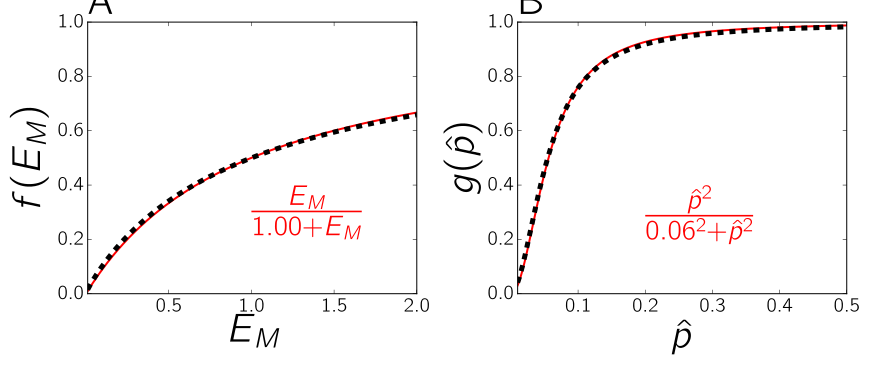
\includegraphics[width=\textwidth]{./Fig/plot_strategies}
\caption{
\noindent\textit{A:} Nutrient-only strategy: $\alpha = f(E_M)$.
The dashed, black curve is the (unique) strategy driving the system exactly to the optimal steady state, that is, the state in which growth occurs at the maximal rate supported by $E_M$.
The function $f$ is defined by Eq.~\ref{eq:meth_f} in the \textit{Methods} section of the main text.
The solid, red curve is an approximation of this function by the simple Michaelis-Menten curve of Eq.~\ref{eq:MMApprox}, with $K_{mE} = 1.0$.
\textit{B:} Precursor-only strategy: $\alpha = g(\hat{p})$.
The dashed, black curve is the (unique) strategy driving the system exactly to the optimal steady state.
The function $g$ is defined by Eq.~\ref{eq:meth_g} in the \textit{Methods} section of the main text.
The solid, red curve is an approximation of this function by the simple Hill curve of Eq.~\ref{eq:HillApprox}, with $K_{mp} = 0.06$ and a cooperativity coefficient 2.}
\end{figure}

%\frontmatter
%\input{Chapters/experiments_summary}
%\mainmatter
\chapter{Monitoring Gene Expression Machinery abundance during a glucose upshift}

\section{Introduction}

\begin{itemize}
\item Understanding growth transitions is important, because so and so.
\item We predicted earlier counter-intuitive bang-bang-singular behaviours for GEM during transition
\item But we're missing experimental data on what really happens in real cells during these transitions (quick review of available data)
\item We fix it by making a strain with fluorescent ribosomes and monitoring ribosome abundance during growth transitions in a microfluidic device.
\end{itemize}

\section{Methods}

\subsection{Strain design}

We used rpsB, GFP, and a chromosomic construction because so and so.

\subsection{Strain construction}

We used Gibson assembly, Kan-pbad-ccdb, etc and obtain the following sequence.

\subsection{Microfluidic device}

Mother machine because needed to change the medium, single cell data because asynchronization etc.

\subsection{Cell segmentation}

We used this and that to analyze the microscopic images.
We applied the following corrections.

\subsection{Kalman smoothing}

We used this and that to analyze the microscopic images.
We applied the following corrections.

\section{Results}

\subsection{Model calibration}

We want to get $\alpha (t)$ during a transition. We show that $\alpha$ can be obtained if we measure so and so.

\subsection{Bang-bang expression during transitions, as predicted}

One stunning figure that show the RFU / cell / pixels, and the predicted $\alpha$ for the glucose-acetate transition.

\subsection{Discrepancies with the model and model adaptation}

The growth rate stalls after the addition of glucose, which was not originally predicted by the model.
This is because so and so.
This can be taken into account if we add another sector (M1 and M2).
This raises a new interesting question : during the transition amino-acids drop, so the cell should produce ribosomes, but it also need to produce the new enzymes to actually be able to perform metabolism.
We thus have competition between several layers of regulation, which can be added to the model by doing so and so.

\section{Discussion}

More research need to be done.

Could be interesting to use transitions for syn bio purposes.
Could be interesting to validate such results in different microorganisms, with different type of medium (fast env, slow env, etc)

\section{Supporting Information}

\begin{itemize}
\item Strain validation (signal-to-noise ratio, growth rate not hampered in microplate reader)
\item Primers used for gibson assembly
\item Difference between mCherry and GFP (mCherry not good because so and so, GFP was chosen)
\end{itemize}

%\frontmatter
%\input{Chapters/discussion_summary}
%\mainmatter
\chapter{Discussion}
\label{chap:discussion}

\textit{"Apples fall onto the Earth because natural selection eliminated apples falling towards the sky."} -- @tomroud~\cite{tomroud_tom_2016}, original source unknown.

\selectlanguage{french}
\section*{Résumé en français}

Dans cette section... (env. 1 page)
\selectlanguage{english}

\begin{center}
\noindent\rule{4cm}{0.1pt}
\end{center}

Physics has yet to be reduced to a formula that will fit on a piece of clothing~\cite{falk_universe_2005}.
This is even more true for Biology, but the extensive work on the mechanisms of evolution are helping to close this gap (see for instance the Price equation, which summarize in a short and elegant formula the mechanisms of evolution and natural selection~\cite{frank_natural_2012}).
But evolution by itself is not sufficient to define life.
Even the less restrictive definition we have -- the one we use to look for life in the universe -- defines a living system as "a self-sustaining chemical system capable of Darwinian evolution"~\cite{deamer_origins_1994,benner_defining_2010}.
Self-sustainment appears to be as fundamental as evolution, and relies on the transformation of matter and energy from the environment into organic matter, in other words, on growth.
But the mathematical framing of questions regarding the self-sustaining character of living systems has not advanced as much as the mathematical analysis of evolution.

Nevertheless, fundamental growth laws have been established for microorganisms.
These growth laws show that, regardless of the molecular mechanisms ensuring growth control, microorganisms tend to follow the same empirical regularities when grown at steady state in different environmental conditions~\cite{molenaar_shifts_2009,scott_emergence_2014,scott_interdependence_2010,scott_bacterial_2011}.
In particular, they adjust their internal molecular composition after a change in the environment, in such a way as to maximize their growth rate~(see in particular~\cite{molenaar_shifts_2009,scott_emergence_2014}).
Growth laws are a strong support for the theory of a modular organization of microorganisms~\cite{scott_emergence_2014,hartwell_molecular_1999,arkin_fast_2006,guido_bottom-up_2006}.
They represent a big step forward towards gaining a general understanding of the physiology of microorganisms.
They have been established at steady state, however, a state in which most microorganisms spend very little time~\cite{mcarthur_microbial_2006,menge_nitrogen_2012,
hobbie_microbes_2013,savageau_escherichia_1983,
savageau_demand_1998,blount_unexhausted_2015,vanelsas_survival_2011}.
Why would microorganisms be optimal for a situation they rarely encounter?
Would known growth laws be specific cases of more general laws allowing microorganisms to respond to changes in the environment?

Our aim in this manuscript has been to establish a theoretical and experimental framework extending growth laws to a dynamical context.
We focused on the growth law describing how ribosome abundance adapts to a change in environment so as to maximize steady-state growth in different media.
Applying the same criterion of growth rate maximization, what is the optimal way to allocate resources during a growth transition between two different environments?
In Chapter~\ref{chap:theory}, we used a simple self-replicator model of resource allocation, and showed that the steady state is invariant over a number of regulatory schemes: the growth rate can be maximized by measuring either the environment or the internal state of the cell.
In both cases, the expression of genes encoding the metabolic and gene expression machineries has to be set to a specific value.
By contrast, biomass maximization during a growth transition requires information about the internal state rather than the environment.
Moreover, expression of the metabolic and gene expression machineries is not set to one specific value, but varies with time in an on-off manner.
What is optimal at steady state and during a growth transition is thus not the same, but this does not mean that a single regulatory system cannot meet both demands.

The model developed here is an instance of proof-of-concept model~\cite{servedio_not_2014}.
It does not necessarily aim at quantitatively predicting or controlling the behavior of microorganisms.
By using a simple and abstract representation, it enables a convenient and tractable way of evaluating the implications of dynamical optimality, in particular its divergence from steady-state optimality.
Is a dynamical perspective on growth laws necessary?
Do regulatory mechanisms need to differ in a dynamical context?
Those are the questions that were investigated by means of this model. 
To our surprise, it additionally provided a new way of looking at the regulatory systems controlling ribosomal abundance in many bacteria.

Some readers might be skeptical about the interest of using such a simple model for addressing the above questions.
Given the profusion of knowledge and data available on biological systems, one might be tempted to introduce every known detail about the molecular implementation of a system of interest.
One of the main drawbacks of such mechanistic models is that we quickly loose track of the big picture and the underlying assumptions.
When including much molecular details, the models also tend to become untractable, prohibiting the use of mathematical tools like optimal control theory that are quickly overwhelmed by the sheer number of variables and parameters in the model.
Besides, simple, abstract models make it easy for the modeler to state the assumptions that are made, and more importantly to identify which ones are logistical, exploratory, or critical (see~\cite{servedio_not_2014}, in particular Box~1).
Logistical assumptions do not affect the conclusions of the model, and are only necessary for tractability.
A good example in our case is the Michaelis-Menten kinetics that were considered in Chapter~\ref{chap:theory}.
Exploratory assumptions, however, might be important to vary and test.
For instance, an exploratory assumption of our model was to consider that the proposed strategies had to be optimal at steady state as well.
This was used as a necessary step to reduce the space of possible solutions, and make the comparison between different strategies time-independent.
Relaxing this assumption would require the exploration of other environmental changes beyond a simple nutrient upshift, but would probably raise interesting considerations~\cite{geisel_constitutive_2011,lopez-maury_tuning_2008,lambert_memory_2014,kussell_phenotypic_2005}.

But the assumptions that are most in need of discussion are the critical assumptions, \textit{i.e.} the ones that are invalidated if the model predictions are not met in nature.
In our case, a critical assumption is that biomass production is the main fitness factor in stable or changing environments.
Throughout the manuscript, we did not really challenge this hypothesis, but only provided arguments about why this assumption is reasonable in some experimental conditions.
The arguments given, however, are mostly based on results obtained with laboratory strains in laboratory conditions.
While it is clear that microorganisms can be cultivated and are even naturally found in conditions where maximizing the growth rate ensures their persistence~\cite{edwards_silico_2001,ibarra_escherichia_2002,lewis_omic_2010,molenaar_shifts_2009}, we have no direct proof that biomass production is the fitness factor that allowed them to naturally persist on evolutionary time-scales.
In addition, one must be careful when explaining the behavior of living systems solely as a consequence of natural selection.
Such systems are embedded in the physical world, and sometimes universal laws just result from the physical limitations that apply to the system (\textit{e.g.}, Monod's law described in Chapter~\ref{chap:introduction}).

The second part of this manuscript was dedicated to setting up an experimental framework for studying resource allocation during growth transitions.
Much emphasis has been given to the experimental issues encountered when studying growth transitions and to come up with possible solutions.
Fluorescent reporter proteins were used to cope with the need for \textit{in-vivo} measurements at high temporal resolution.
Advances in microfluidics were exploited to perform steady-state-to-steady-state transitions following a change in medium, in order to buffer the effect of the pre-culture history~\cite{ng_damage_1962,dufrenne_effect_1997,shaw_effect_1967}.
Finally, the signal of interest was reconstructed through the use of Kalman smoothing, a powerful signal processing algorithm that has, as we showed, many features that make it suitable for the analysis of microscopy time-series data~\cite{kailath_linear_2000,jazwinski_stochastic_2007,kalman_new_1960}.
Overall, the set-up still needs many improvements, though most of them are experimental issues that should be easily fixable.

Chapter~\ref{chap:experiments} must not be taken as a "test of the model" in Chapter~\ref{chap:theory}, but rather as a test of its assumptions (see Box~2 in~\cite{servedio_not_2014}).
The model is correct in that bang-bang resource allocation follows mathematically from the assumption that microorganisms maximize their biomass production at steady state and during growth transitions.
The model predictions can be used, however, as a tool to test whether this critical assumption is valid.
In Chapter~\ref{chap:experiments}, we thus apply the experimental set-up to observe the resource allocation profile following a nutrient upshift in \textit{E.~coli}.
While we were not able to arrive at an unambiguous conclusion about the correctness of the model prediction in this manuscript, we can draw up two possible scenarios in the wake of future improvements of the experimental set-up.

In one scenario, the bang-bang or at least oscillatory nature of resource allocation during a growth transition is confirmed.
This would suggest that the regulatory mechanisms of resource allocation do maximize biomass production during growth transitions, hence that microorganisms are adapted for changing environments.
In order to further establish these results, we would need additional data for a broader range of environmental conditions.
The most straightforward extension would be to test other upshift and downshift schemes (different carbon sources, amino-acids supplementation, nitrogen instead of carbon limitation, ...).
The experimental set-up could also be slightly modified to test a broader range of variables.
For instance, the strain could be modified so as to express an additional fluorescent protein that would report the abundance of a key enzyme of metabolism.
Along with the ribosomal reporter, this would allow us to test the prediction that the metabolic and gene expression machineries are expressed in anti-phase.

In the other scenario, we do not observe any trace of a bang-bang resource allocation scheme.
In that case, the questions that would arise are which critical assumptions are not valid.
We also cannot discard the possibility that an assumption that was originally identified as exploratory or logistical might in fact be critical for the predictions of the model.
Although unlikely \textit{a priori}, this might be the case for the expressions used for the macroreactions in the model (Eqs~\ref{eq:metaflux}-\ref{eq:machflux}), the definition of the volume as invariably proportional to the total mass of macromolecules (Eq.~\ref{eq:voldef}), or the fact that degradation is assumed negligible with respect to the rates of other reactions in the system.
More probably, the assumptions regarding the cost of the regulatory system could be more critical than initially thought.
By only comparing the regulatory schemes with respect to their benefits, we implicitly made the assumption that their costs are negligible or at least comparable.
The costs of regulatory schemes are actually difficult to model~\cite{shachrai_cost_2010,dong_gratuitous_1995,dekel_environmental_2005}, since the cellular variables are not equally costly to measure and, as we showed for the ppGpp system, one mechanism may measure several variables at once.
Nevertheless, relaxation of this hypothesis would definitively need to be explored before concluding that microorganisms do not optimize their biomass production during growth transitions.

In any case, exploring the costs of regulatory mechanisms might uncover a fundamental link between the complexity of the regulatory schemes and the dynamics of the environment.
As we illustrated in Chapter~\ref{chap:theory}, complex regulatory schemes only prove beneficial in a dynamical context, away from steady state.
At the opposite extreme, one can expect the benefits of these regulatory schemes to saturate, whereas the cost of complexity would probably not saturate, since acquiring more information is expected to require additional sensing systems, diverting away an increasingly larger part of cellular resources.
Overall, these two tendencies are expected to cross at a point that would represent an evolutionary bottleneck, beyond which the costs exceed the benefits (see~\cite{short_flows_2006} for another example of such a bottleneck).
Interestingly, the position of the bottleneck might be dependent on the environment, resulting in a dynamic law that would link the complexity of regulatory systems to the dynamics of the environment.
In other words, while the current growth laws consider how the physiology of the cell varies with the nutrient quality of the medium, we could add another dimension representing the time-varying availability of this nutrient in the natural environment.

\bibliography{references}

\end{document}

